% !TeX spellcheck = <none>
\documentclass[12pt, english]
{article}

\usepackage{graphicx}
\usepackage{subfig}
\usepackage{microtype}
\usepackage[automake, nonumberlist, acronym, toc, section]{glossaries}
\usepackage{cite}
\usepackage[parfill]{parskip}
\usepackage{amssymb}
\usepackage{textcmds}
\usepackage{hyperref}
\usepackage{float}
\usepackage[toc,page]{appendix}
\usepackage{marginnote}
\usepackage{xcolor}
\usepackage{booktabs}

\newglossary[slg]{symbolslist}{syi}{syg}{Symbols}

\makeglossaries

%commands for symbols
\newglossaryentry{symb:Pi}{
name=$\pi$,
description={You know it.},
sort=symbolpi, type=symbolslist
}
\newglossaryentry{symb:Phi}{
name=$\varphi$,
description={At vero eos et accusam et justo duo dolores et ea rebum..},
sort=symbolphi, type=symbolslist
}
\newglossaryentry{symb:Lambda}{
name=$\lambda$,
description={Lorem ipsum dolor sit amet, consetetur sadipscing elitr, sed diam nonumy.},
sort=symbollambda, type=symbolslist
}
 
%commands for abbreviations

% ...

%abbreviations and glossary combined
\newacronym{AD}{AD}{Active Directory\protect\glsadd{glos:AD}}
\newacronym{t-SNE}{t-SNE}{t-Distributed Stochastic Neighbor Embedding}
\newacronym{pca}{PCA}{Principal Component Analysis}
\newacronym{ari}{ARI}{Adjusted Rand Index}
\newacronym{ami}{AMI}{Adjusted Mutual Info Score}
\newacronym{sc}{SC}{Silhouette coefficient}
\newacronym{mi}{MI}{Mutual Information}
\newacronym{dbscan}{dbscan}{Density-Based Spatial Clustering of Applications with Noise}
\newacronym{minPts}{MinPts}{Minimum number of points to be considered in Eps-neighourhood for DBSCAN}

 
% ... 
 
%glossary commands

\newglossaryentry{glos:K-Algorithms}{
name=K-Algorithms,
description={One of the studied clustering algorithms, that work with a parameter k: K-Means, K-Medians, K-Medoids}
}

\newglossaryentry{glos:onehotencoding}{
	name=One-Hot-Encoding,
	description={Encoding method for categorical attribute values where every attribute is represented as a binary vector and each element in the vector represents a category.}
}

\newglossaryentry{glos:rangequery}{
	name=RangeQuery,
	description={Function to find all points in a Eps-Neighbourhood around a given point.}
}
% ...

\patchcmd{\subequations}{\def\theequation{\theparentequation\alph{equation}}}%
{\def\theequation{\theparentequation.\arabic{equation}}}{}{}

\begin{document}

\begin{titlepage}

\begin{center}

{\Huge {
Term Paper Data Science 1}
}
\\[2ex]

\textbf{
\Large 
Docent: Prof. Dr. Lena Wiese \\ 
Semester: Summer Term 2021\\  
}




\includegraphics[scale=0.4]{logo.jpg} \\ 
\large{\textbf{Institute of Computer Science \\ Goethe-Universit\"at Frankfurt a. M.}}



\begin{tabular}{ll}
Authors: & \textsc{Franziska Hicking} \\
& {\small 6673525} \\
& {\small franziska.hicking@stud.uni-frankfurt.de} \\
& {\small Master Bioinformatics, 2} \\
& \textsc{Jonas Elpelt} \\
& {\small 6673181}\\
&{\small  elpelt@stud.uni-frankfurt.de}\\
& {\small Master Bioinformatics, 2} \\
& \textsc{Julian Rummel} \\
&{\small  6673334}\\
& {\small s9594673@stud.uni-frankfurt.de}\\
&{\small  Master Bioinformatics, 2} \\
& \textsc{Niklas Conen}\\
& {\small 6599913}\\
& {\small conen@stud.uni-frankfurt.de}\\
& {\small Bachelor Computer Science, 8}\\
Date: & \today \\		
\end{tabular}

\end{center}

\vspace*{\fill}

\large
\noindent{}Chosen Project Topic: \\
T4 - DISTANCE MEASURES AND CLUSTERING \\
\small Github Repository: \url{https://github.com/elpelt/datascience1\_group42/}




\end{titlepage}

\newpage%\thispagestyle{empty}~ %empty page
All authors confirm that they contributed equally to the project report and were involved in the implementation and evaluation to the same extent.
\newpage 

\begin{abstract}
Clustering algorithms can be important tools during the analysis of datasets. They divide a dataset into groups of items based on a certain measure of similarity such as the distances between each of the items. 
In this work, we implemented and compared four different clustering algorithms (K-Means, K-Medoids, K-Median, DBSCAN). For this, we selected four distinct datasets as well as multiple distance measures (Manhattan, Euclidean, Angular cosine, Chebyshev). For efficient comparison of the clustering results we made use of multiple clustering indices. Additionally, we implemented a web frontend which provides the ability to run all clustering algorithms with distance measures, datasets and clustering indices chosen by the user. The results will be visualized afterwards.
After running all algorithms with each of the datasets respectively and all distance measures where they could be applied, we compared the resulting values of the clustering indices.
Finally we tried to estimate the best parameter combinations for each dataset.

\end{abstract}

\newpage

\tableofcontents

\newpage


\section{Definition of Distance Measure}
\label{def_DM}
A distance measure is a function $d(x, y)$ that calculates a real value between two points in a space, containing two sets of points. If $d(x, y)$ satisfies the following three axioms the distance measure is classified as a \textit{metric}:
\begin{subequations} \label{metricaxioms}
    \begin{align}
        d(x, y) &= 0 \Leftrightarrow x = y &&\text{Identity of indiscernibles}\\
        d(x, y) &= d(y, x) &&\text{Symmetry}\\
        d(x, y) &\leq d(x, z) + d(z, y) &&\text{Triangle inequality}
%
\intertext{
    The triangle-inequality imposes the condition that a distance reflects the shortest path between two points. Thus, it is not possible to achieve a distance improvement by traveling via an intermediate point $z$. \cite{MMDS} \endgraf
    Moreover all axioms enforce non negative distances as an additional condition.
}
        d(x, y) &\geq 0 &&\text{No negative distances} \label{metricnonnegative}
    \end{align}
\end{subequations}

\section{Different Distance Measurements} \label{distances}
\subsection{Manhattan Distance}
To determine the distance between two items the Manhattan distance, also referred to as taxicab distance, may be used. This distance measure assumes a n-dimensional vector space with a fixed cartesian coordinate system. It is defined as following \cite{Craw2010}:
\begin{align}
	d(x,y) = ||x-y||_1 = \sum\limits_{i=1}^{n}|x_i - y_i|
\end{align}
where x and y are vectors
\begin{align*}
	x = (x_1, x_2,..., x_n) \text{ and } y = (y_1, y_2,..., y_n)
\end{align*}

The Manhattan distance is, like the Euclidean distance, part of the $L_p-metrics$ (see section \ref{lpmetric}), where the value for $p$ is set to 1.
Assuming a two dimensional space, the distance between two points is the shortest path between them with the restriction of only being able to move vertically and horizontally.\\
Prove of axioms described in section \ref{def_DM}:\\
\begin{enumerate}
	\item Identity of indiscernibles:\\
	Let $x=y$, then $|x-y| = 0$ and hence $\sum\limits_{i=1}^{n}|x_i - y_i| = 0$
	\item Symmetry:\\
	This axiom is fulfilled since $|x-y| = |y-x|$ for any x and y , which implies that $\sum\limits_{i=1}^{n}|x_i - y_i| = \sum\limits_{i=1}^{n}|y_i - x_i|$.
	\item Triangle inequality:\\
	$|x-y| \leq |x-z|+|z-y|$ holds true for any $x,y,z \in \mathbb{R}$
	This means that for $\sum\limits_{i=1}^{n}|x_i - y_i| = \sum\limits_{i=1}^{n}|x_i - z_i| + \sum\limits_{i=1}^{n}|z_i - y_i|$ the equation $|x_i - y_i| \leq |x_i - z_i| + |z_i - y_i|$ is true for each i which in turn shows that the axiom is fulfilled.
	\item Non-Negativity:\\
	This condition is trivial since the Manhattan distance is a sum of absolute values and can therefore never be negative.
\end{enumerate}
\subsection{Euclidean Distances}
The Euclidean distance is part of the $L_p$\textit{-metrics} which are defined as
\begin{align} \label{lpmetric}
    d(x, y) = \sum_{i=1}^{n}(|x_i-y_i|^p)^\frac{1}{p}
\end{align}
Setting $p = 2$ expresses the Euclidean distance, which is defined as the positive square root of the sum of all squared distances in each dimension:
\begin{align}
    d(x, y) = \sqrt{\sum_{i = 1}^{n}(|x_i - y_i|)^2}
\end{align}

The first two axioms defined in section \ref{def_DM} are easily shown to apply:
\begin{enumerate}

\item Identity of indiscernibles:\\
For $x = y$ the value is obviously $0$. Let $x = y$, then $(|x - y|)^2 = 0$ and $\sqrt{0} = 0$.

\item Symmetry: \\
Symmetry is cleary given by the square of each distance.\\
$(x - y)^2 = (y - x)^2$.
\end{enumerate}

Non negativity is also shown quite easily. The square of any real number is always positive and the squareroot of any real positive number is always positive. Hence $d(x, y) \geq 0$.\\
\ \\
The traingle inequality requires a more difficult proof. However, to keep it simple, the Euclidean space possesses the property that the sum of the lengths of Cathetus and Ancathetus is always longer than the length of the Hypothenuse. \cite{MMDS}

\subsection{Angular Cosine Distance}
The angular cosine distance gives the (normalized) angle between two points $x$ and $y$ represented as vectors in an $n$-dimensional space. It does not make a difference between a vector and a multiple of that vector. The cosine distance can be calculated by applying the arc-cosine function to the cosine of the angle $\theta$ between $x$ and $y$ \cite{MMDS}. \\
It is based on the cosine similarity (cosine between two vectors $x$ and $y$), which is definied as: \\

\begin{equation}
	\text{cosine similarity} = \frac{\sum_{i=1}^{n} x_i y_i}{\sqrt{\sum_{i=1}^{n} x_i^2 \sum_{i=1}^{n} y_i^2}}
\end{equation}  

The cosine similarity, however, is not a distance as it is defined for positive values only. Therefore it has to be converted to the normalized angle between $x$ and $y$ as followed \cite{cosdist}: \\

\begin{equation}
	\text{angular cosine distance} = \frac{\arccos({\text{cosine similarity})}}{\pi}
\end{equation}  

Note, that if $x$ or $y$ are zero vectors, the cosine similarity would not be defined. To prevent a division by zero the cosine similarity is set to 1 in this special case (based on the implementation of the pairwise distance in scikit-learn). 

The axioms for a distance measure are fulfilled for the cosine distance \cite{MMDS}: \\

\begin{enumerate}
	\item Identity of indiscernibles:\\
	Two vectors can have a cosine distance of 0 if and only if they are located in the same direction. (This applies also to vectors that are multiples of one another and therefore are in the same direction.) 
	\item Symmetry: \\
	Symmetry is obviously given by the equality to measure an angle between $x$ and $y$ and an angle between $y$ and $x$. 
	\item Triangle inequality: \\
	A rotation from $x$ to $y$ can be explained by a rotation from $x$ to $z$ and then to $y$. Therefore a sum of these two rotations is always bigger or equal than the rotation directly from $x$ to $y$ 
	\item No negative distances:\\
	Regardless of the dimensionality of the space the values of the cosine distance are between 0 and 180 degrees, therefore no negative distances can occur. 
	
\end{enumerate}



\subsection{Chebyshev Distance}
The Chebyshev distance (also known as Tschebyscheff distance, Maximum Value distance or $L_\infty$ distance) is the limit of the before mentioned $L_p$-metrics (equation \ref{lpmetric}). On a vector space this metric is induced by the Supremum Norm (also called Chebyshev Norm or Infinity Norm), which again is the limit of the $L_p$-norms.\\
Descriptively the Chebyshev metric is the greatest distance between two vectors on one axis. Formally it is defined as:
%
\begin{align}
    d(x, y) = \max (| x_i - y_i |)
\end{align}
%
which is the aforementioned limit of the $L_p$-metric and is therefore also called $L_\infty$-metric:
\begin{align}
    d(x, y) = \lim \limits_{p \to \infty} \left( \sum_{i=1}^{n}(|x_i-y_i|^p)^\frac{1}{p} \right)
\end{align}
\ \\
The three axioms for a metric (section \ref{metricaxioms}) are proven below:
\begin{enumerate}
    \item For $x = y$ all entries of a vector are identical all differences between $x_i - y_i$ are $0$. Thus: $d(x,x) = \max (|x_i - x_i|) = \max (0) = 0$
    \item Symmetry is given because of the symmetry of the absolute value function: 
          $| x_i - y_i | = | y_i - x_i |$
    \item The triangle equation can be shown using some estimates:
    \begin{align*}
        \max(| x_i - y_i |) &= \max(|x_i - z_i + z_i - y_i|)\\
         &\leq \max(|x_i - z_i|+ |z_i - y_i|) \\
         &\leq \max(| x_i - z_i |) + \max(|z_i - y_i|)\\
        \Rightarrow d(x,y) &\leq d(x, z) + d(z, y)
    \end{align*}
\end{enumerate}
Non negativity also results from the non negativity of the absolute value function.


\section{Data Set Description}

\subsection{Housevotes} \label{housevotes}

The housevotes dataset, created by Jeff Schlimmer in April 1987, was taken from the UCI Machine Learning Repository \cite{Dua2019}. The dataset consists of voting results of Congressmen of the U.S. House of Representatives on 16 key votes during the second session of Congress in 1984. The key votes and the voting results are identified by the Congressional Quarterly Almanac (CQA) documenting this session of Congress. The voting results are split into nine different types by the CQA, which are consolidated into three results used in the dataset.\\
\ \\
Voted for, paired for, and announced for count as a yes vote (y in the dataset).
Voted against, paired against, and announced against count as a no vote (n in the dataset).
Voted present, voted present to avoid conflict of interest, and did not vote or otherwise make a position known are denoted as a unknown state (? in the dataset).\\
\ \\
The set consists of 435 data points with 16 dimensions and can be grouped into two classes, 267 democrats and 168 republicans.\\
\ \\
The distance based cluster algorithms described in section \ref{algorithms} all need numerical data in order to find clusters. Therefore the categorical data of this dataset needs to be encoded in a way that accurately describes the distance between the datapoints. The voting data has no order and all voting results have the same distance to one another. Hence the dataset was one-hot-encoded.\\
With \Gls{glos:onehotencoding} every attribute is represented as a binary vector. Each element of this vector represents a category value. The corresponding value of a sample is set to 1 in the binary vector. 
This increases the dimensionality of the problem, but represents an equal distance between every value an attribute can have.\\


\subsection{Wine}
\marginnote{\textcolor{blue}{Jonas Elpelt}}
This dataset contains the chemical analysis results of Italian wines from 3 different cultivators. It is also taken from the UCI Machine Learning Repository \cite{Dua2019}. 
The dataset consists of 178 instances, each of them having 13 numeric attributes according to different measurements taken for different constitutuents (alcohol, malic acid, ash, alcalinity of ash, magnesium, total phenols, flavanoids, nonflavanoid phenols, proanthocyanins, color intensity, hue, OD280/OD315 of diluted wines, proline). Each instance belongs to either one of three classes containing 59, 71 and 48 data points. 
It was created by R. A. Fisher in July 1988 \cite{scikitlearn}. 
\subsection{Iris}
The Iris Dataset, introduced by Ronald Fisher in 1936, contains the petal and sepal measurements of three different species of Iris flowers \cite{fisher1936use}. The considered irises are Setosa, Versicolour and Virginica and each flower is represented in its own class. For each iris, 50 samples are included and for each sample the entirely numerical dataset contains the sepal length, sepal width, petal length and petal width in cm. Hence, the dataset consists of four columns where each represents one of the mentioned measurements and 150 lines, one for each individual flower. This dataset can be classified as multivatiate as there are four different features for each instance. \\
Although is dataset is comparatively small with only 150 instances in total, it is widely known and very popular for various statistical classification methods such as machine learning and support vector machines \cite{inproceedings}. Due to its popularity, it is not only included in the UCI Machine Learning Repository \cite{Dua2019}, but also in the base version of R \cite{rbase} and in the Python Scikit-learn package \cite{scikitlearn}.\\
While one species of iris is linerally seperable from the other irises, the other two are not linerally seperable from each other \cite{Dua2019}. This makes this dataset an interesting case for clustering.
\subsection{Diabetes} \label{diabetes}
The diabetes dataset contains various information as numeric values about 442 diabetic patients, namely age, sex, body mass index, average blood pressure, and six blood serum measurements (first 10 columns), as well as a quantitative measure of disease progression one year after baseline, i.e., the response of interest (11th column). All characteristics were standardized to standard deviation times $n$ samples and also mean centered.\\
This dataset is taken from the diabetes study conducted by Efron et al. \cite{diabetes} with the main goal of constructing a model that predicts the response (column 11) from the covariates (column 1-10).\\
Compared to all other datasets, it has no pre-classification of the data. Thus, there are no predefined clusters and thus no external cluster validation methods can be used for evaluation. Hence, the silhouette score is implemented and should be used for evaluation purposes.


\section{Clustering Algorithms} \label{algorithms}
\subsection{K-Means}
% !TeX spellcheck = <none>
The K-means algorithm aims to group together similar items of a given dataset into clusters. 
The total number of clusters is predefined and represented as the value for k. All considered items can be referred to as points, as this clustering algorithm assumes an Euclidean space. Hence, only distance measures which assume an Eulicdean space, such as the Manhattan distance or the Euclidean distance, are sensibly appicable. The K-means algorithm belongs to the point-assignment algorithms in clustering, as all points are considered successively and assigned to the most fitting cluster. The algorithms operates in the following steps: \cite{MMDS}
\begin{enumerate}
	\item Initially, the algorithm picks k points whose positions each represent one cluster centroid
	\item All points are considered in turn:
	\begin{itemize}
		\item Find the nearest centroid/mean of the considered point (Euclidean distance measure at default)
		\item Assign point to cluster of that centroid
		\item Adapt position of this centroid
	\end{itemize}	
	
	\item (optional) fix all centroids and reassign all points with the inclusion of the initial k points
	
\end{enumerate}

The essential first step of initializing the clusters requires $k$ points that have a high chance of being in separate clusters. This can be achieved by different approaches. One possible approach consists of picking points which are as far away as possible from each other. This can be achieved by the conducting the following steps:
\begin{enumerate}
	\item	A random point is picked as the first of $k$ cluster centorids
	\item	For k-1 passes: \\
	Pick the point whose minimum distance is the largest considering all previously chosen points
	
\end{enumerate}
Another way of determining the cluster centroids is the K++ initializer, described in section 5, which we used in our implementation of the K-means algorithm.\\
After the K-means algorithm assigned all points, an optional step af reassigning the points with fixed centroids can be conducted. This can be sensible since it is possible that after a point has been assigned to cluster the centroids move so far that the point would now belong to a different cluster.\\
The K-means clustering algorithm has many advantages including its simplicity which makes it easy to implement and its guaranteed convergence meaning it will always find a solution. The linear runtime of this algorithm is another advantage. However, a disadvantage is that the value for k has to be predetermined. This means that the algorithm might have to be run multiple times. Additionally, the starting points of the centroid greaty effect the outcome of the algorithm.

\subsection{K-Medoids}
The K-Medoids clustering method is related to the well-known K-means algorithm, but uses medoids (representative points for each cluster) instead of means to define new cluster centers, which makes it more robust to outliers.\cite{Jin2010} It partitions the dataset by assigning each data point to the closest of $k$ cluster centers, which are defined by the most centrally located medoids. A medoid is a point with a minimal average dissimilarity to all other data points in the same cluster. The most commonly used algorithm to solve this NP-hard problem heuristically is the PAM (Partitoning Around Medoids) algorithm, that works as following: \cite{kaufman2009finding} \\
\begin{enumerate}
	\item First initialize the algorithm by selecting $k$ data points to be the medoids and assigning every data point to its closest medoid. \\
	\item Compare the average dissimilarity coefficient of a swap of each medoid $m$ and a non-medoid data point $\bar{m}$. Find a swap between $m$ and $\bar{m}$ that would decrease the average dissimilarity coefficient the most. 
	\item If no change of a medoid happened in the second step, terminate the algorithm, else re-assign the data points to the new medoids and go back to step 2. 
\end{enumerate}

\subsection{K-Median}
The K-Medians cluster algorithm is closely related to the K-Means algorithm, but is more robust to outliers because it uses the median as statistics in order to determine the center of each cluster. Its main approach is to cluster data by minimizing the absolute deviations, corresponding to the Manhattan distance, between each point and its closest cluster center, i.e., creating $k$ disjoint cluster by minimizing the following function. \cite{kmed}
\begin{align}
    Q(\{\pi_j\}^K_{j=1}) = \sum_{j=1}^{K}\sum_{x \in \pi_j}||x-c_j||_1
\end{align}
The geometric median is used for the minimization.
\begin{align}
    {{arg\, min}\atop{y\in\mathbb{R}^n}} \sum_{i=1}^m ||x_i-y||_2
\end{align}
At the start of the algorithm, k cluster centers must be initialized. There are many different approaches to perform this task, such as Random Initialization, Density Analysis, Single Dimension Subsets, and many more. In this work, the random approach was used because many of the other theories, while theoretically promising, are inferior or nearly equivalent in performance to the results produced by random initialization. \cite{kmed} Achieving global optimization in K-Medians is known to be NP-complete \cite{kmed_time}.\\ 
The algorithm works as following:\cite{algo_kmed}
\begin{enumerate}
    \item Assign each datapoint to a cluster, thus its nearest cluster center using the Manhattan distance as default (it can be substituted for a different distance measure) 
    \item Shift the cluster centers to the position of the vector whose elements are equal to the median value of each dimension of all instances in a cluster.
    \item There is no guarantee to get the perfect cluster because the starting cluster centers were initialized randomly. There is the approach of reinitializing the algorithm many times and securing the best cluster center of all iterations.
\end{enumerate}
The runtime of the K-medians algorithm is, similarly to the K-Means algorithm, $O(ntk)$. Due to the algorithms similarity to the K-Means algorithm, the advantages and diadvantages apply here as well.\\

\subsection{DBSCAN}

DBSCAN was developed by Martin Ester, Hans-Peter Kriegel, Jiirg Sander and Xiaowei Xu. All following definitions and descriptions are taken from their original publication \cite{dbscan} or their revisit of DBSCAN \cite{dbscanrevisited} and only apply to this algorithm.\\
Contrary to the aforementioned centroid-based partitioning algorithms (k-means, k-medoids and k-median) the DBSCAN (\textit{Density Based Spatial Clustering of Applications with Noise}) algorithm uses point densities to determine clusters.\\
To introduce the definition of the density of a cluster, first the Eps-neighbourhood of a point is defined:\\
\ \\
\textbf{Definition 1:} \textit{Eps-neighbourhood}\\
A point q is part of the Eps-neighbourhood $N_{Eps}$ of point p if the distance between them is smaller than a threshold distance called Eps.\\
The Eps-neighbourhood therefore is defined as $N_{Eps} = \{q \in D \ | \ ||p, q|| \leq Eps \}$ with $D$ denoting the entirety of points that are supposed to be clustered and $||p, q||$ being the distance between p and q for an arbitrary distance measure.\\
\ \\
The Eps-neighbourhood fails at being a reliable measure for the point density if a point is located at the border of a cluster. These points are called \textit{border point}. Points that are located on the inside of a cluster are called \textit{core points}. Hence the following definition is made:\\
\ \\
\textbf{Definition 2:} \textit{directly density-reachable and density-reachable}\\
A point p is directly density-reachable from a point q when
\begin{enumerate}
    \item $p \in N_{Eps}(q)$
    \item $|N_{Eps}(q)| \geq \text{MinPts}$
\end{enumerate}
with \acrshort{minPts} being the minimal number of points that $N_{eps}(q)$ should contain so that q is considered a core point of a cluster.\\
A point is \textit{density-reachable} if there is a chain of points between $p$ and $q$ so that all neighbouring points in the chain are directly density reachable.\\
\begin{figure}[H]
    \centering
    \subfloat[eps-neighbourhood ]{{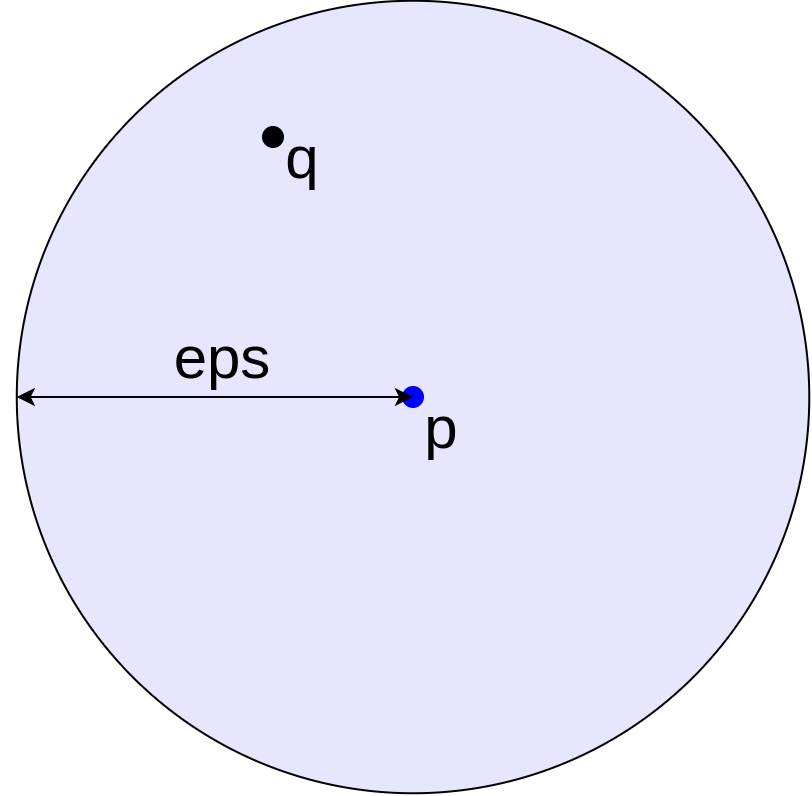
\includegraphics[height=7em]{./images/eps-neighbourhood}}}
    \qquad
    \subfloat[direct density-reachable]{{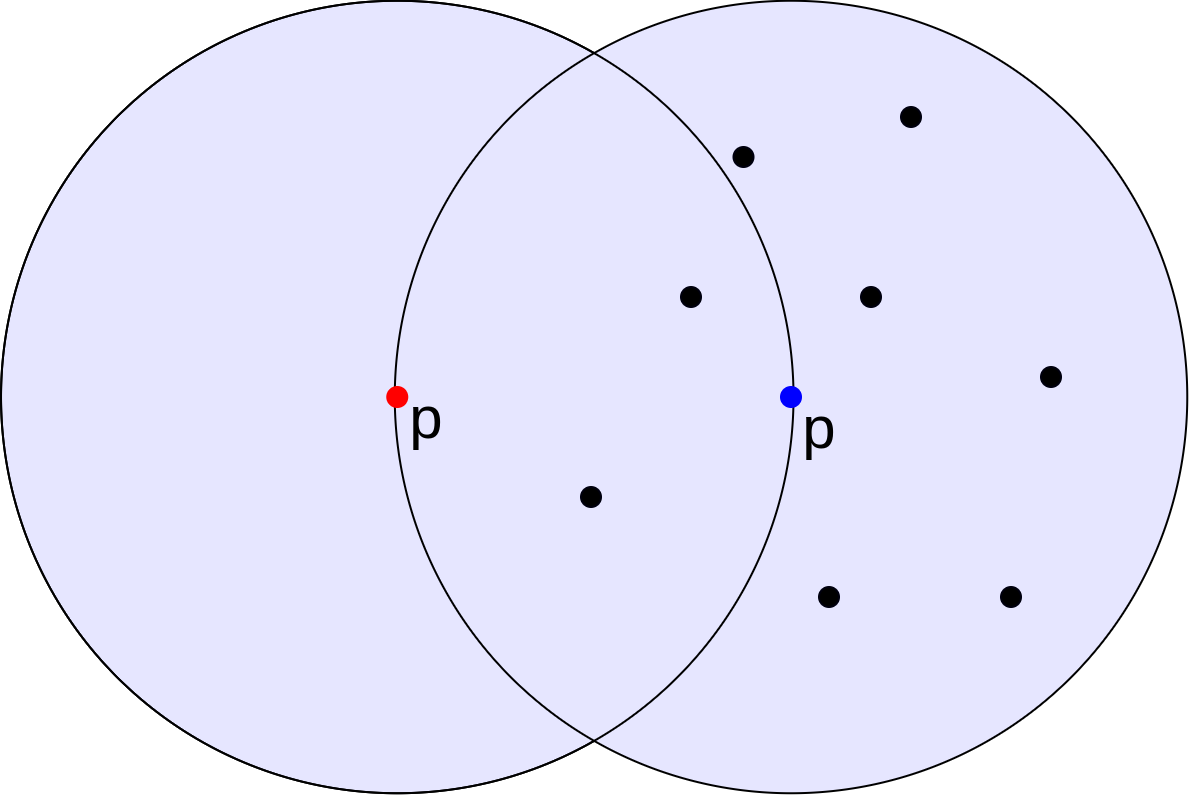
\includegraphics[height=7em]{./images/direct-density-reachable} }}
    \caption{visualisations of the definitions for eps-neighbourhood (left) and direct-density-reachable (right)}
\end{figure}
\ \\
To complete the definition of what is considered part of a cluster density-connectivity is defined:\\
\ \\
\textbf{Definition 3:} \textit{density-connected}\\
Two points $p$ and $q$ are considered density-connected if there is a common point $o$ which is density-reachable from $p$ and $q$.\\
\ \\
\begin{figure}[H]
    \subfloat[density-reachable]{{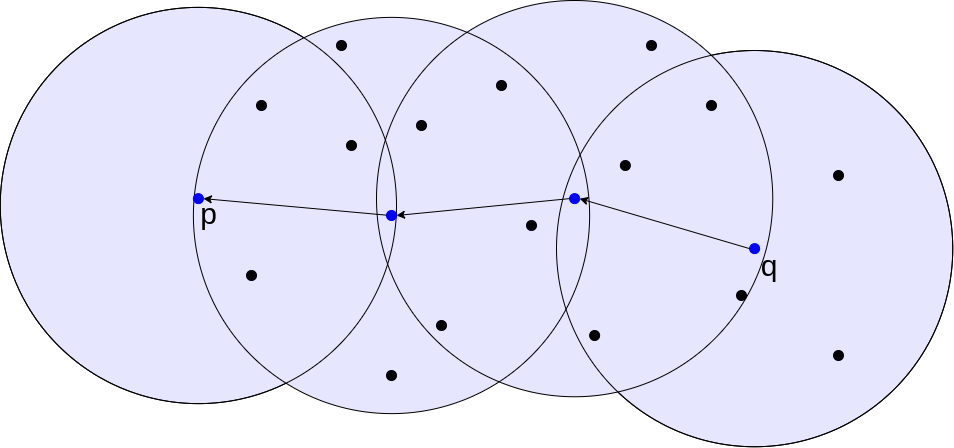
\includegraphics[height=7em]{./images/density-reachable} }}
    \subfloat[density-connected]{{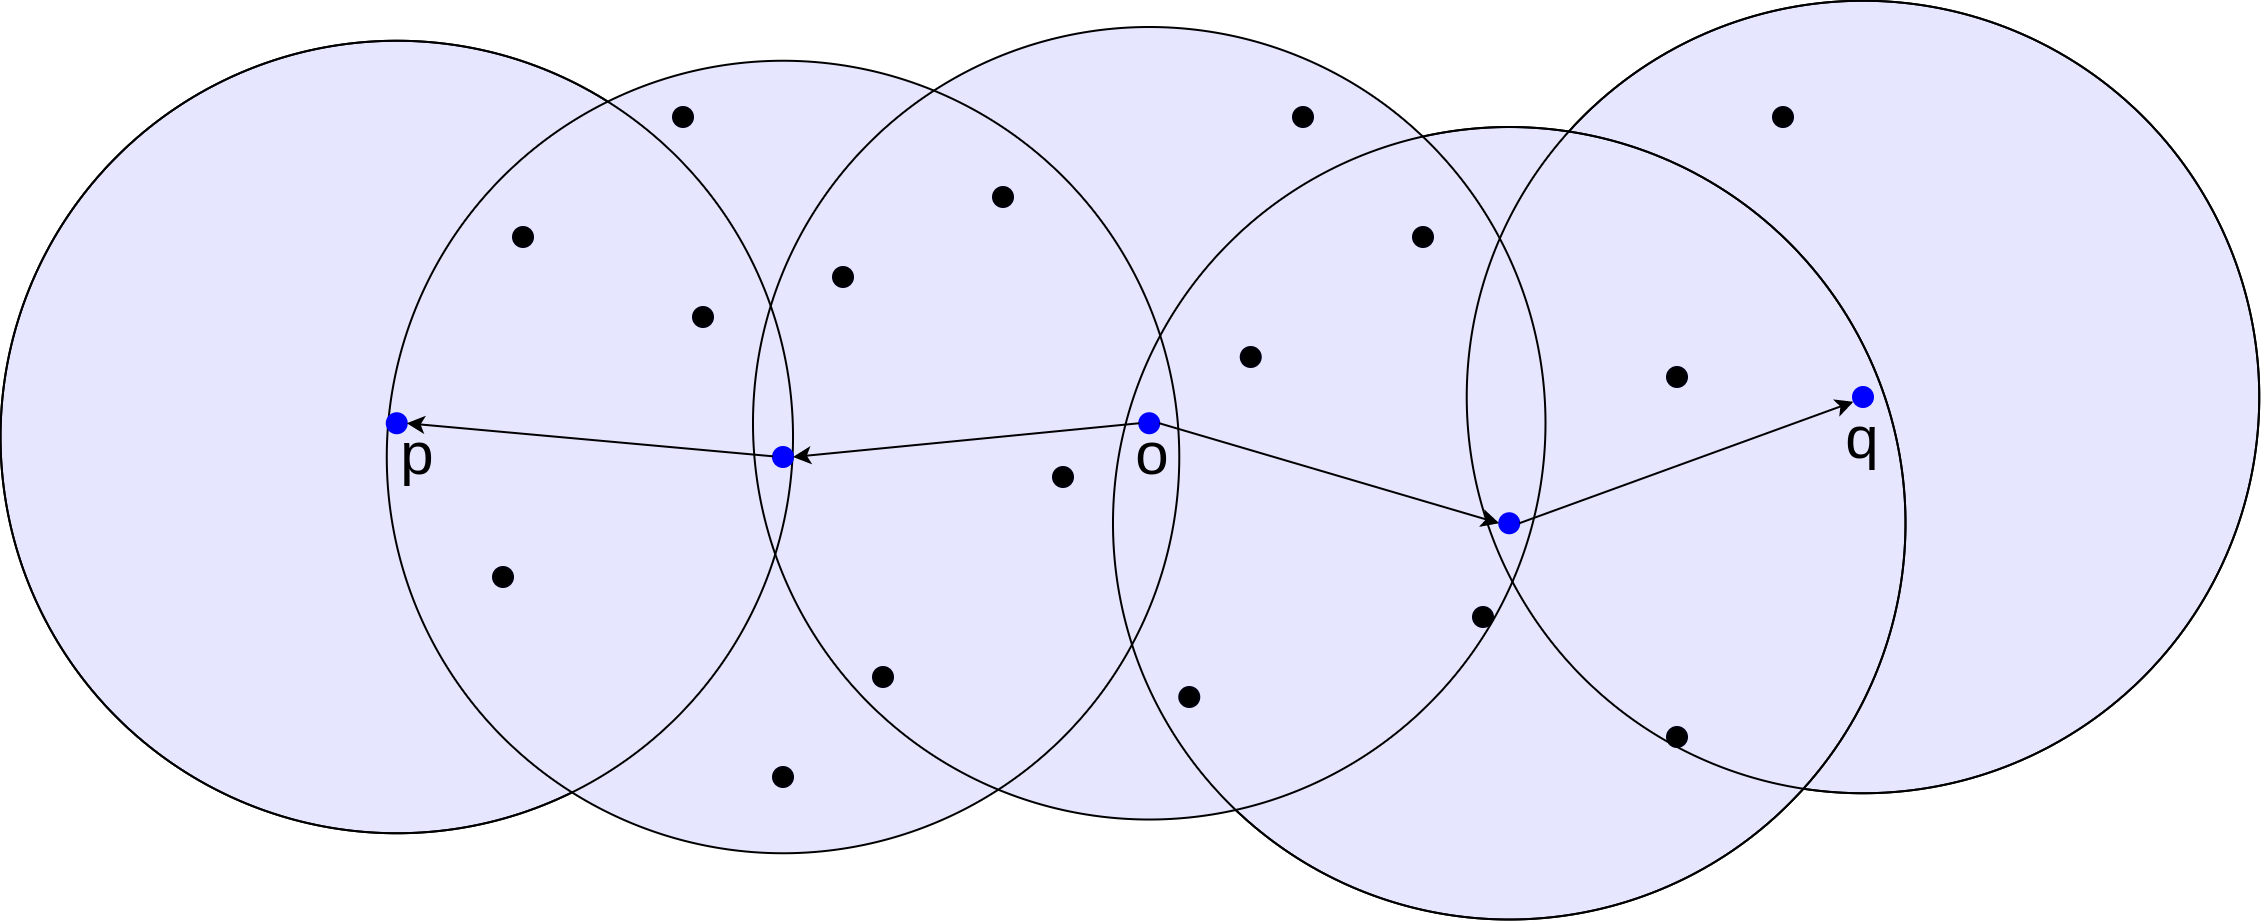
\includegraphics[height=7em]{./images/density-connected} }}  
    \caption{visualisations of the definitions for density-reachable (left) and density-connected (right)}
\end{figure}
Now a cluster can be described as:\\
\ \\
\textbf{Definition 4:} \textit{cluster and noise}\\
A cluster is a non empty subset $C \in D$ so that:
\begin{enumerate}
    \item $\forall p, q: p \in C \wedge q \text{ is density reachable from } p \Rightarrow q \in C$
    \item $\forall p, q \in C: \ p$ is density-connected to q
\end{enumerate}
\textit{Noise} is easily defined as every point that is not part of a Cluster $C_i$.\\
\ \\
Using these definitions DBSCAN can start the clustering process with given values for Eps and MinPts. First all points are marked as not labeled. Starting from an arbitrary point $p$ all points are iterated through in a linear fashion. For each point a \texttt{\Gls{glos:rangequery}} function is executed finding all directly density-reachable neighbours of $p$. If less then minPts neighbours are found, $p$ is labeled as noise. Otherwise $p$ is a core point and is labeled as part of the currently explored cluster. If this is the case the neighbourhood of $p$, from now on denoted as S, is expanded.\\
\ \\
Unlabled points get checked for the core point condition (which equals a \texttt{RangeQuery} call) and all subsequent found neighbours are also added to S. Points that got labeled as Noise beforehand and are part of S are labeled as part of the cluster.
When the expansion comes to an end a cluster is yielded, the next unlabeled point is chosen as $p$ and DBSCAN will continue to look for a new cluster.\\
\ \\
The biggest advantage of DBSCAN is its capability to find oddly shaped or spatially complex clusters. The aforementioned partitioning algorithms all fail at finding clusters that are not shaped like a sphere or a ellipsoid, if they are spatially entangled. scikit-learn published a great comparision of clustering algorithms on their website where the capabilities of DBSCAN are visualised \footnote{\url{https://scikit-learn.org/stable/auto_examples/cluster/plot_cluster_comparison.html}}. An example of DBSCANs capabilities generated using the python script on the aforementioned site is shown in figure \ref{fig:dbscanadv}.\\

Moreover DBSCAN allows for clustering without knowing the exact number of clusters or a termination criterion. Though finding the best values for minPts and eps can be equally challenging. The heuristic described in section \ref{dbscanheuristic} tries to simplify the estimation of these parameters.
\begin{figure}
    \centering
    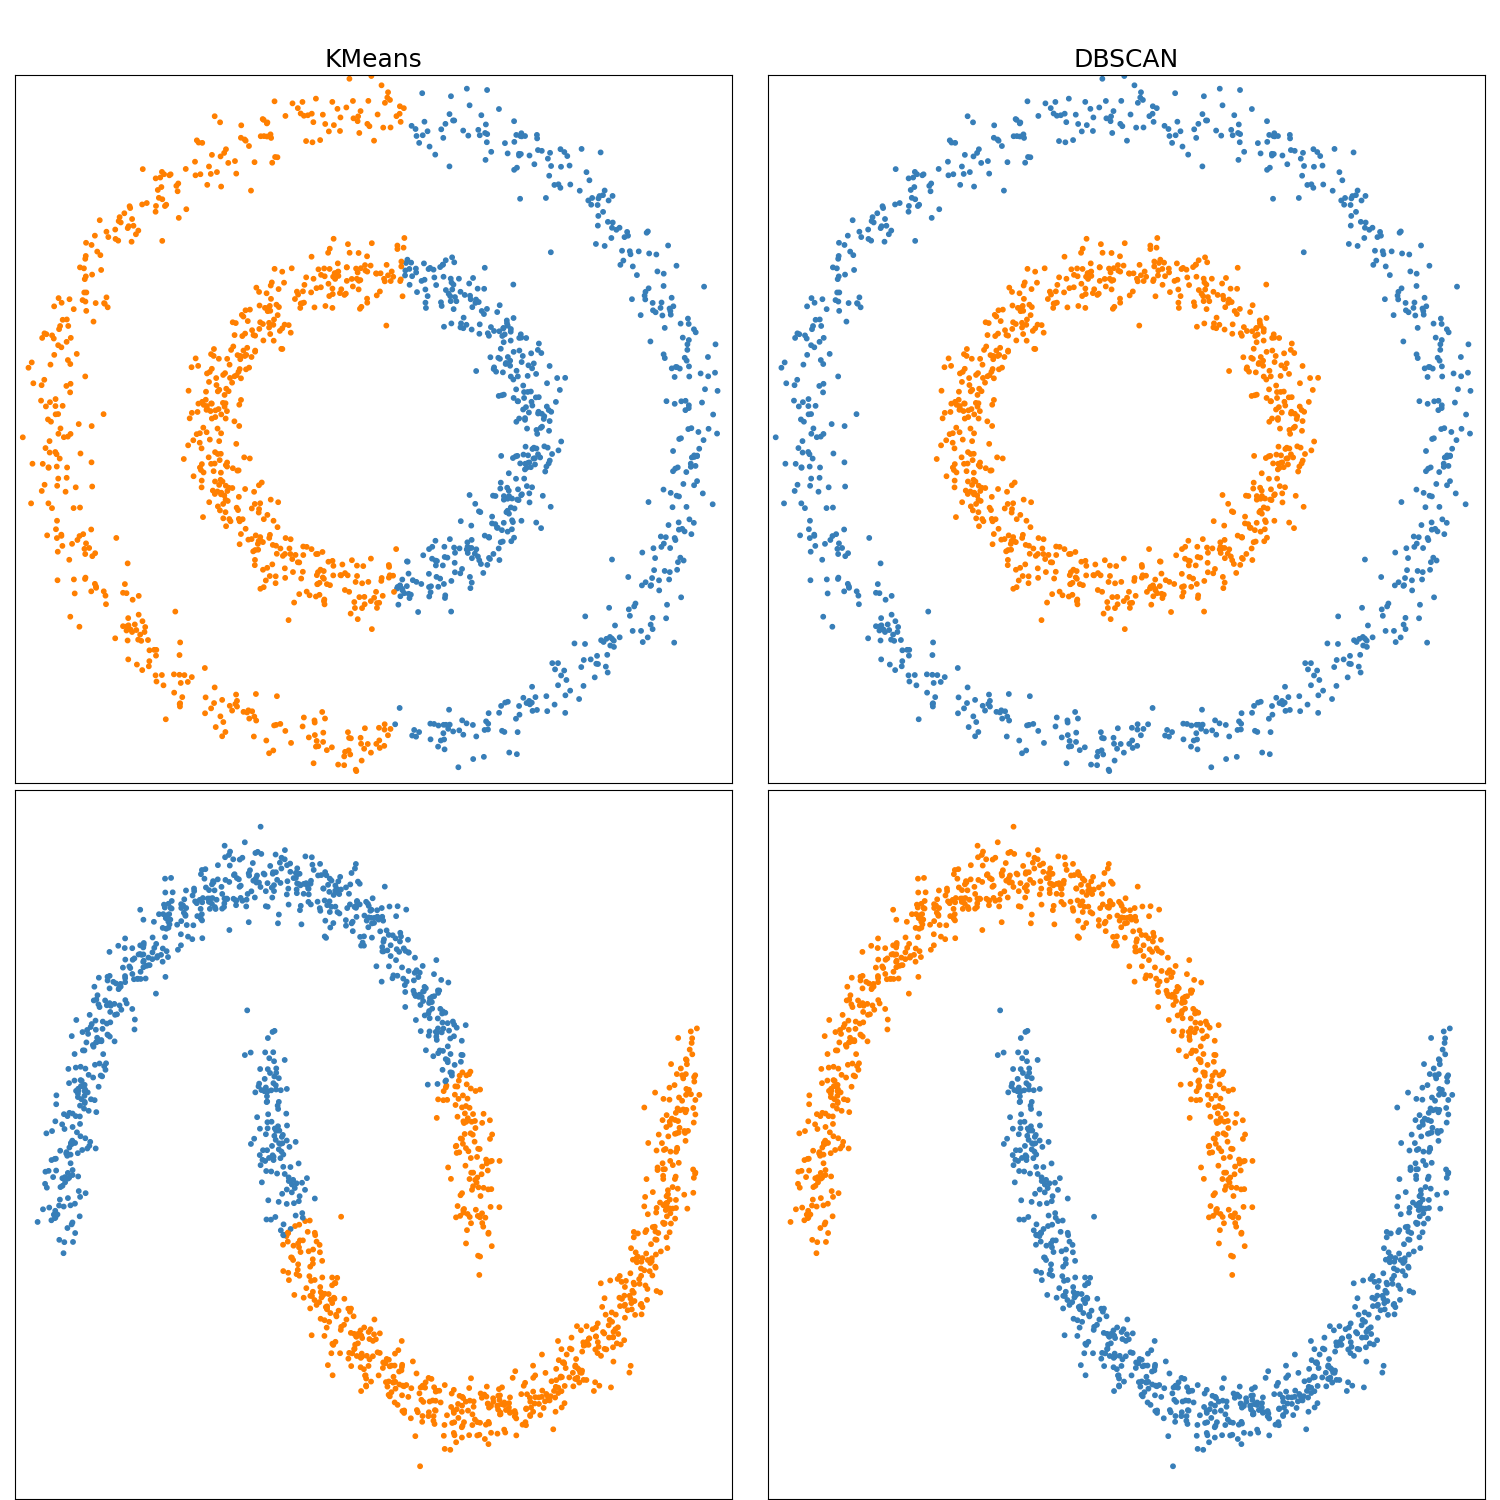
\includegraphics[width=0.4\textwidth]{../plots/dbscan/dbscan_comp}
    \caption{Comparision of DBSCAN to kmeans on spatially complex clusters}
    \label{fig:dbscanadv}
\end{figure}

Lastly DBSCAN will fail at finding multiple clusters if they are spatially close to each other. Because of the nature of the eps-neighbourhood all clusters with points seperated by a distance equal or less less than eps can not be distinguished.

The runtime complexity of DBSCAN heavily depends on the runtime of the \texttt{RangeQuery} function which is executed for every point in the dataset once.
If \texttt{RangeQuery} is implemented using a linear scan, its complexity will be $\Theta (n \cdot D)$ with $D$ being the time needed for calculating the distance between points. Therefore the runtime complexity of DBSCAN is $\Theta(n^2 \cdot D)$ \cite{dbscanrevisited}.

\section{Additional Methods Used}
\subsection{k++-Initializer}
%K++ initializer
The K++ initializer is a method which determines the positions of the initial $k$ cluster centroids before starting the K-means algorithm. The following steps outline how the K++ initializer operates:

\begin{enumerate}
	\item Choose one centroid at random from all possible datapoints.
	\item Loop through all remaining datapoints (k-1):\\
	determine the distance $D(x)$ of the datapoint to the nearest already chosen centroid using the Euclidean distance.
	\item A weighted probability distribution is used to set the next cluster centroid. For each point, the probability to be chosen is proportional to $D(x)^2$, meaning points which are farther away are more likely to be chosen.
	\item Steps 2 and 3 are repeated until all $k$ cluster centroids have been set.
	
\end{enumerate}

\subsection{t-SNE}

\acrfull{t-SNE} is a nonlinear dimensionality reduction technique, which was developed by Laurens van der Maaten and Geoffrey Hinton \cite{tsne}. It can be used for visualizing high-dimensional data in a lower-dimensional (typically 2-dimensional) space such that more similar data points should be represented nearby in the lower-dimensional representation. This can lead to visual cluster formation based on the local structure of the data (and chosen parameters) \cite{wattenberg2016how}.  \\
The t-SNE algorithm first calculates the distances $d(x_i, x_j)$ (by default using the euclidean distance) between each of the $N$ data points $x_i$ and $x_j$ \cite{tsne_matlab}. Then it computes conditional probabilities $p_{j|i}$, \qq{ that $x_i$ would pick $x_j$ as its neighbor if neighbors were picked in proportion to their probability density under a Gaussian centered at $x_i$.}\cite{tsne} \\
$p_{j|i}$ for $i \neq j$ is given as
\begin{equation}
	p_{j|i} = \frac{exp(-d(x_i, x_j)^2 / 2\sigma_i^2)}{\sum_{k \neq i} exp(-d(x_i, x_k)^2 / 2\sigma_i^2)} 
\end{equation}
and $p_{i|i} = 0$ is set. \\
The joint probability $p_ij$ is defined by 
\begin{equation}
	p_{ij} = \frac{p_{j|i} + p_{i|j}}{2N}
\end{equation}

Note that the Gaussian distributions should have their standard deviations $\sigma_i$ such that the perplexity of the conditional distribution is equal to a predefined perplexity parameter \cite{tsne_matlab}. It basically measures the effective number of neighbours of the data point $i$, that can be found performing a binary search.   \\
In the next step t-SNE searches for an embedding of the data points considering the previously computed similarities \cite{tsne_matlab}. This is achieved by minimizing the Kullback-Leibler divergence between the modeled Gaussian distributions of the high-dimensional data points $X$ and a Student t distribution of the corresponding points $Y$ in the lower-dimensional space. To do this we define $q_{ij}$ for $i \neq j$ as followed 
\begin{equation}
	q_{ji} = \frac{(1 + \lVert y_i - y_j \rVert ^2)^{-1}}{\sum_{k}\sum_{l \neq k} (1 + \lVert y_k - y_t \rVert ^2)^{-1}}
\end{equation}
and set $q_{i|i} = 0$. \\
Now the Kullback-Leibler divergence can be expressed as \\
\begin{equation}
	KL(P||Q) = \sum_{j}\sum_{i \neq j}p_{ij}\log\frac{p_{ij}}{q_{ij}}
\end{equation}

The optimization procedure is performed by a gradient descent method to find a local minimum \cite{tsne_matlab}. \\
The final results may heavily depend on the chosen parameters, especially the perplexity value \cite{wattenberg2016how}. It is therefore recommended to compare different perplexity values to identify spurious clustering artifacts in the visualization.

\subsection{Principal Component Analysis (PCA)}
PCA is a dimension reduction technique to increase interpretability while minimizing information loss during the process. Working with a dataset containing $p$ numerical variables and $n$ entities, a $n$x$p$-Matrix $X$ gets defined with $p$ vectors as columns. Now linear combinations (see: \ref{lin_comb}) of the columns of $X$ with maximum variance (see: \ref{var}) are searched for, given by: 
\begin{align}\label{lin_comb}
    \sum_{j=1}^{p}a_jx_j = Xa
\end{align}
\begin{align}\label{var}
    var(Xa) = a^TSa
\end{align}
with $a$ as vector of constants $a_1,...,a_p$ and $S$ as sample covariance matrix associated with the dataset. \cite{pca_beg}\\
These linear combinations are called principal components and are $p$ uncorrelated, new variables for the initial variables. Most of the information of the original data is compressed in the first principal component, with reduced but maximized information in the following components. It is highly important to understand the correlation between variance and information. The greater the variance, the greater the dispersion and thus the greater the abundance of information. Eigenvectors and eigenvalues are needed to calculate the principal components, where the eigenvectors of the covariance-matrix $S$ are the directions of the axes where most of the variance is present and the corresponding eigenvalues indicate the amount of variance contained in each principal component. \cite{pca_step} This produces the equation: \cite{pca_beg}
\begin{align}
    Sa - \lambda a = 0 \Leftrightarrow Sa = \lambda a
\end{align}
Thus, ranking the eigenvectors in order of their eigenvalues, one obtains all principal components from 1 to $p$. In the following step, the user can decide whether to keep all principal components or discard some of them based on their calculated significance, by: \cite{pca_beg}
\begin{align}
    \pi_j = \frac{\lambda_j}{\sum_{j=1}^{p}\lambda_j}
\end{align}
This results in a matrix called feature vector, which contains all the remaining components as columns and forms the final dimension of the reduced data set \cite{pca_step}. Usually, the requirements of graphical representation lead to keeping the first two to three principal components \cite{pca_beg}. Finally, the original data gets reorientated from the original axes to the axes represented by the principal components.
\subsection{DBSCAN Parameter Estimation Heuristic} \label{dbscanheuristic}
In the original publication of the DBSCAN algorithm \cite{dbscan} a simple way for approximating the MinPts and Eps parameters was proposed.

The described heuristic defines a function \texttt{k-dist} which calculates the distance d of each point to its k-nearest neighbour.
The d-neighbourhood of each point then contains k+1 points in most cases. Theoretically it could happen that two points share the same distance d to a point. Then the d-neighbourhood could contain more than k+1 points though this case is most unlikely.

Sorting the resulting distances in decending order and plotting them against the points results in the so called \textit{sorted k-dist graph}. This graph gives some insights about the datasets density distribution. Choosing any point in this graph, setting MinPts to k and Eps to the k-dist value of the point, will result in DBSCAN classifying every point with the same or smaller k-dist value as a core point. These points will therefore be assigned to a cluster. Points with a larger k-dist value could be, but do not have to be, classifyied as noise. 

In the sorted k-dist graph a threshold point can be searched describing the maximal distance of the thinnest cluster. The DBSCAN paper \cite{dbscan} proposes a visual approach on finding such threshold points by looking for a kind of bend or "valley" in the graph. 
In figure \ref{fig:sorteddistgraphiriseucl} an example is shown for such a bend found in the 4-dist graph of the iris dataset, using the euclidean distance.

\begin{figure}[H]
    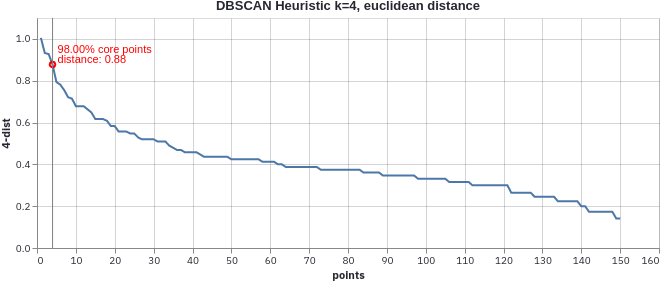
\includegraphics[width=0.92\textwidth]{../plots/dbscan/iris_4dist_euclidean}
    \caption{sorted 4-dist graph for Iris dataset and euclidean distance}
    \label{fig:sorteddistgraphiriseucl}
\end{figure}

While this method provides good results for some datasets, sometimes the estimated parameters do not produce a meaningful clustering or a bend may not be visible in the sorted k-dist graph. In some cases the distance chosen may result in one large cluster. Then eps must be reduced until DBSCAN can find multiple clusters, most likely resulting in more noise.

An interactive display of this heuristic with adjustable parameters for all datasets was also created using streamlit and altair and is hosted on streamlit sharing 
\footnote{\scriptsize\url{https://share.streamlit.io/elpelt/datascience1_group42/main/code/heuristic_web.py}}.
The plot in figure \ref{fig:sorteddistgraphiriseucl} was created using this interface.


\section{Implementation}
\subsection{Description}
The application follows an object oriented approach. To unify the implementation of all cluster algorithms a base class, not meant for actual instanceing, was defined aggregateing all functions that the cluster algorithms need.
The cluster algorithms themselves are implemented as child classes inheriting all methods and attributes from the base clustering class. This allows setting different parameters for every cluster algorithm while guaranteeing the existence and uniform execution of methods used by all algorithms.

\begin{figure}[H]
    \centering
    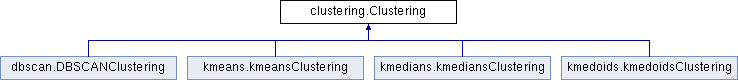
\includegraphics[width=0.9\textwidth]{../docs/html/classclustering_1_1Clustering}
    \caption{Inheritance diagramm for the cluster algorithm classes}
\end{figure}

Three different libraries were used for their implementations of the used cluster algorithms. 
For K-Means and K-Medians the pyclustering \cite{Novikov2019} implementations were used, because of their flexibility in setting custom distance measures. For K-Medoids the scikit learn extra \cite{scikit-learn-extra} implementation was used.
DBSCAN is realised using the scikit learn implementation \cite{scikitlearn}.

To reduce time spent on computing a class for organising already calculated resulsts as json files was created. All clustering results using the option of a predefined fixed seed are, if available, loaded from a file, or are calculated and then saved. Optionally cluster results can be bulk computed using a given script (\textit{result\_calculation.py}). Because of the large amount of possible parameter combinations of DBSCAN we decided to precompute only results for K-Means, K-Medians and K-Medoids with $k$ ranging from 1 to 10 for all distance measures.

The calculation of cluster indices is packaged into a Indices class and uses scikit learn implementations of the different scoring methods. Clustering results used for index calculations are saved using a data structure called SessionState. This structure is written by Thiago Teixeira \cite{sessionstate} implementing a way of saving parameters per session. That is for example a browser tab in which the interface is opened. The variables saved in the SessionState are persistent until a session is closed, eventhough streamlits framework is designed in a way, where every page is a sequential python script being completely reloaded when an action is triggered. 

Finally the webfrontend is implemented using streamlit and is hosted using their sharing service \footnote{\scriptsize\url{https://share.streamlit.io/elpelt/datascience1_group42/main/code/web_frontend.py}}. The cluster plots are generated using either seaborn or altair given a flag one can set in the frontend. The scoring results are visualised using matplotlib. The graphs which are visualised using altair are interactive in the way, that the user can freely move and zoom through the plots. By hovering over a point informations about this plot are shown in a small popup window. Where possible streamlits cacheing decorator is used, to reduce loading times when using any widget on the webpage.

Additionally the DBSCAN heuristic described in section \ref{dbscanheuristic} was also implemented using streamlit and interactive altair charts for displaying the results. All utility functions for the heruistic were packaged into a class and are then called from the script implementing the frontend. The finished page is also hosted on streamlit share \footnote{\url{https://share.streamlit.io/elpelt/datascience1_group42/main/code/heuristic_web.py}} and is linked to from the projects webfrontend, when choosing DBSCAN as clustering algorithm.

All of the code base for the project is documented using the Doxygen style and an automatically generated documentation containing detailed description of every class, method and attribute can be accessed through the github projects page \footnote{\url{https://elpelt.github.io/datascience1_group42}}.
\subsection{Dependencies}
Multiple libraries were used for their implementation of cluster algorithms and other functionality needed for working with results and visualising them. Below follows a brief description of all used libraries.

\subsection{pyclustering}
pyclustering is a data mining library, focusing on clustering algorithms written in C++ and Python by Andrei Novikov \cite{Novikov2019}. The library contains a wide range of clustering algorithms implemented in Python with an optional C++ core. If possible pyclustering falls back to its C++ implementations utilising its efficiency and runtime benefits.\\
We use pyclusterings implementation of K-Means and K-Medians.

\subsection{scikit learn}
scikit learn is a wide rangeing data analysis tool kit for python encompassing algorithms not only for clustering but for classification, regression and more \cite{scikitlearn}.\\
The library is used for its implemntations of DBSCAN, One-Hot-Encoding, StandardScaler, TSNE and PCA.

\subsection{scikit learn extra}
scikit learn extra is an extension to scikit learn spanning algorithms that do not satisfy the inclusion criteria of scikit learn. This library is used for its implementation of K-Medoids that is fully compatible with all other scikit learn algorithms.

\subsection{numpy}
numpy is a fundamental library mostly used for its array structure implementing a C++/Fortran like way of saveing and organising data while still being relatively easy to use. Being a dependency of every other package used in this project we use numpy arrays to store and work with our datasets.

\subsection{seaborn}
seaborn is a powerful data visualisation library build on top of pythons matplotlib. seaborn simplyfies plotting predefined templates. We use seaborns \texttt{scatterplot} template for visualising the TSNE and PCA projections of the cluster results.

\subsection{streamlit}
streamlit is a easy-to-use library for building simple web apps. Our webfrontend is implemented in streamlit and is also hosted on their sharing service.\\
\\
----- TODO ----- Link zur gehosteten app

\section{Evaluation Module}
\subsection{Implementation}
All indices are implemented as a class function for the class Indices(). The code is part of the scikit-library \cite{scikitlearn} and expects two inputs for external cluster validation methods and three input for the internal cluster validation method. The input contains two arrays, namely the computed cluster labels and the expected cluster labels from the original data. For the internal index, the input is expected to be the calculated labels, the original data points, and a metric to calculate the distances (default = selected metric for cluster calculation). As output, a numerical value between 0 and 1 is calculated for homogeneity score, completeness score, and adjusted mutual index. For the adjusted rand index and the internal index silhouette score a value between -1 and 1 is calculated.\\
The user can add all scores to a comparison using a data structure called SessionState. All added calculations are visualized in the form of an interactive histogram created with Altair.  

\subsection{External Scoring Methods}
\subsubsection{Definition}
Validation of clustered data is a fundamental challenge in the clustering problem. To obtain a comparable and evaluable numerical value, validity indices are usually used. There are many different indices calculating this value in different ways. For example, external cluster validation scores. External criteria are defined as the evaluation of the result with respect to a given structure, here given as a classification in the original data. Thus, an external index compares the predefined cluster labels with the set of computed labels and returns a value based on the differences and similarities respectively. In short, it is based on previous knowledge of the data. \cite{int_ext}
\subsubsection{Adjusted Rand Index}
\acrshort{ari} is an external cluster validation method with a value between -1 and 1, where a value close to 0 represents a random partitioning and a value close to 1 represents a nearly identical cluster compared to the original labels of the data. Thus, maximizing this score argues for perfect clustering.\\
It is defined by \cite{ari}: 
\begin{align}
    ARI(P^*,P) = \frac{\sum_{i,j}\binom{N_{i,j}}{2}-[\sum_{i}\binom{N_{i}}{2}\sum_{j}\binom{N_{j}}{2}]/\binom{N}{2}}{\frac{1}{2}[\sum_{i}\binom{N_{i}}{2}+\sum_{j}\binom{N_{j}}{2}]-[\sum_{i}\binom{N_{i}}{2}\sum_{j}\binom{N_{j}}{2}]/\binom{N}{2}}
\end{align}
$N$ is the number of data points in the dataset and $N_{i,j}$ describes the number of data points in a class label $C_j^* \in P^*$ associated with cluster $C_i$ in partition $P$. $N_i$ represents the number of data points in cluster $C_i$ of partition $P$, while $N_j$ represents the number of data points in class $C_j^*$ \cite{ari}. 
\subsubsection{Completeness Score}
The Completeness Score is another external clustering index. Essentially, the Completeness Score determines how many items with the same labeling are also put into the same cluster. It is symmetric to the Homogeneity Score and is defined as following \cite{rosenberg2007v}:
\begin{align}
    c = 1 - \frac{H(K|C)}{H(K)}  
\end{align}
where
\begin{align}
    H(C|K) = - \sum_{c,k} \frac{n_{ck}}{N}\log\left(\frac{n_{ck}}{n_c}\right)  
\end{align}


Consistent to the Homogeneity Score, C represents the true cluster labels of the datapoints and K the labels predicted by the clustering algorithm. $n_{ck}$ is the number of items in a cluster $k$, which are labeled $c$, i.e. share the same label. $n_c$ stands for the total number of points labeled $c$.
When all items labeled $c$ are put into one single cluster $k$, the Completeness Score is 1.
\subsubsection{Homogeneity Score}
The homogeneity score is an external clustering index to determine the quality of a calculated clustering in comparison to a preexisting grouping of items.
It is defined as following: \cite{rosenberg2007v}\\

\begin{align}
    h = 1 - \frac{H(C|K)}{H(C)}
\end{align}
where
\begin{align}
    H(C|K) = - \sum_{c,k} \frac{n_{ck}}{N}\log\left(\frac{n_{ck}}{n_k}\right)
\end{align}

Here, C represents the true cluster labels of the datapoints and K represents the labels predicted by the clustering algorithm. $n_{ck}$ is the number of items in a cluster $k$, which are labeled $c$, i.e. share the same label. $n_k$ stands for the total number of labels present in cluster $k$.
When each cluster $k$ conains only items with the same label $c$, the homogeneity score equals one.
\subsubsection{Adjusted Mutual Index}
The Adjusted Mutual Info Score (AMI) is an external cluster valdidation method, in order to calculate the informativeness of a partition computed by a clustering algorithm. It is an adjustment of the Mutual Information (MI) Score to account for chance \cite{scikitlearn}. This score is upper bounded by 1 and is expected to be 0 for random partitions. The score is calculated as following: \cite{ari_form}
\begin{align}
    AMI_{max}(U,V) &= \frac{NMI_{max}(U,V)-E\{NMI_{max}(U,V)\}}{1-E\{NMI_{max}(U,V)\}}\\ &= \frac{I(U,V)-E\{I(U,V)\}}{max\{H(U), H(V)\}-E\{I(U,V)\}}
\end{align}
$NMI$ stands for Normalized Mutual Index, which is the Mutual Index normalized to values in the range of 0 to 1 \cite{scikitlearn}. $E\{I(U,V)\}$ is the calculated expected index and $I(U,V)$ the actual Index \cite{ari_form}.
\subsection{Internal Scoring Methods}
\subsubsection{Definition}
In addition to external cluster valdiation indices, there are also internal indices. These indices are based on internal criteria, defined as the evaluation of the result in terms of an information inherent in the data alone. This is needed for datasets where no predefined classification is given, such as the diabetes dataset. Compared to external indices, internal indices are known to be more accurate in determining group in a given clustering structure, but show poorer time complexity. \cite{int_ext}
\subsubsection{Silhouette Score}
The Silhouette Score is an internal cluster validation method that calculates the mean silhouette coefficient (SC) of all samples \cite{scikitlearn}. It calculates a separation distance between resulting clusters, by stating how close each point in one cluster is to the points in a neighboring cluster \cite{sil_score}. The score is calculated as following: \cite{scikitlearn}

\begin{align}
    SC = \frac{b-a}{max(a,b)}
\end{align}

for each sample. $b$ is defined as the distance between the distance between a sample and the nearest cluster to which the sample does not belong, and $a$ as the mean intra-cluster distance.\\
The silhouette coefficient can be calculated either for each cluster or the entire dataset. To obtain a comparable value, in this project the score for the entire dataset is calculated as the mean value over all samples. \cite{scikitlearn}\\
This index is necessary to compare the different results for the clustering of the diabetes dataset, since this dataset does not contain a predefined classification.


\section{Web Frontend and User Manual}
The web frontend is designed to provide an intuitive exploration of the different datasets, clustering algorithms and distances. In an interactive interface multiple clustering settings can be chosen and a visualisation of the results is directly generated. 
A cluster-table is used to store previous calculated results, which can be plotted within the evaluation module. \\
The checkbox \qq{Use precalculated results (with random seed for reproduction)} at the top of the page (see \autoref{fig:parameters} A), which is set by default, allows the use of precalculated clustering results, which have been computed beforehand (with a random seed value) and are stored in the github repository. This was done for reproduction and runtime purposes. The second checkbox "use interactive charts" (see \autoref{fig:parameters} B), also set by default, allows the option for interactive projection plots for \acrshort{pca}, \acrshort{t-SNE}, and the evaluation module.  \\
The user can choose between four datasets (see \autoref{fig:parameters} C), four distance measures (see \autoref{fig:parameters} E) and four different algorithms (see \autoref{fig:parameters} D) via a drop-down menu. If one of the K-Algorithms is chosen a value for the parameter k between 1 and 10 has to be set (see \autoref{fig:parameters} F). The default value for k is 3. If DBSCAN is chosen the user has to define a value for Eps and MinPts. (see \autoref{fig:dbscan_para} A). Additionally, a link to a webpage implementing the DBSCAN heuristic described in section \ref{dbscanheuristic} is shown. A short manual for this page is given in section \ref{heuristicmanual}. The parameter settings can be adjusted with interactive slider widgets. \\
\begin{figure}[H]
	\centering
	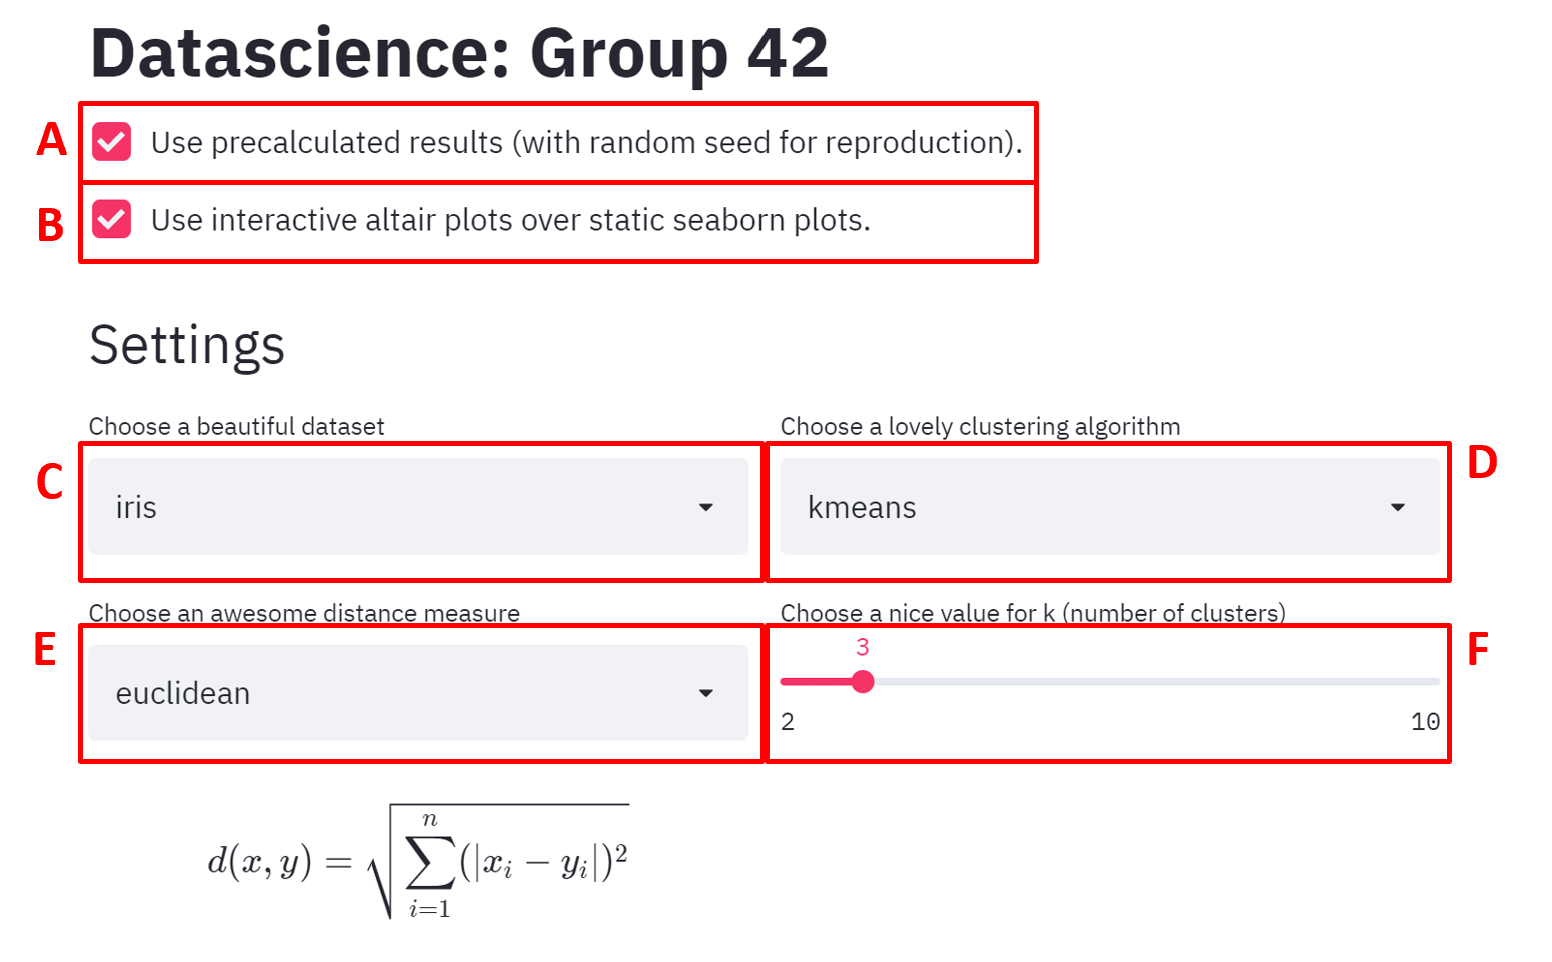
\includegraphics[width=\linewidth]{modules/web_frontend/eingabe_letters}
	\caption{First part of the web frontend. Setting options for clustering parameters for K-Means, K-Medians and K-Medoids.}\label{fig:parameters}
\end{figure}
\begin{figure}[H]
	\centering
	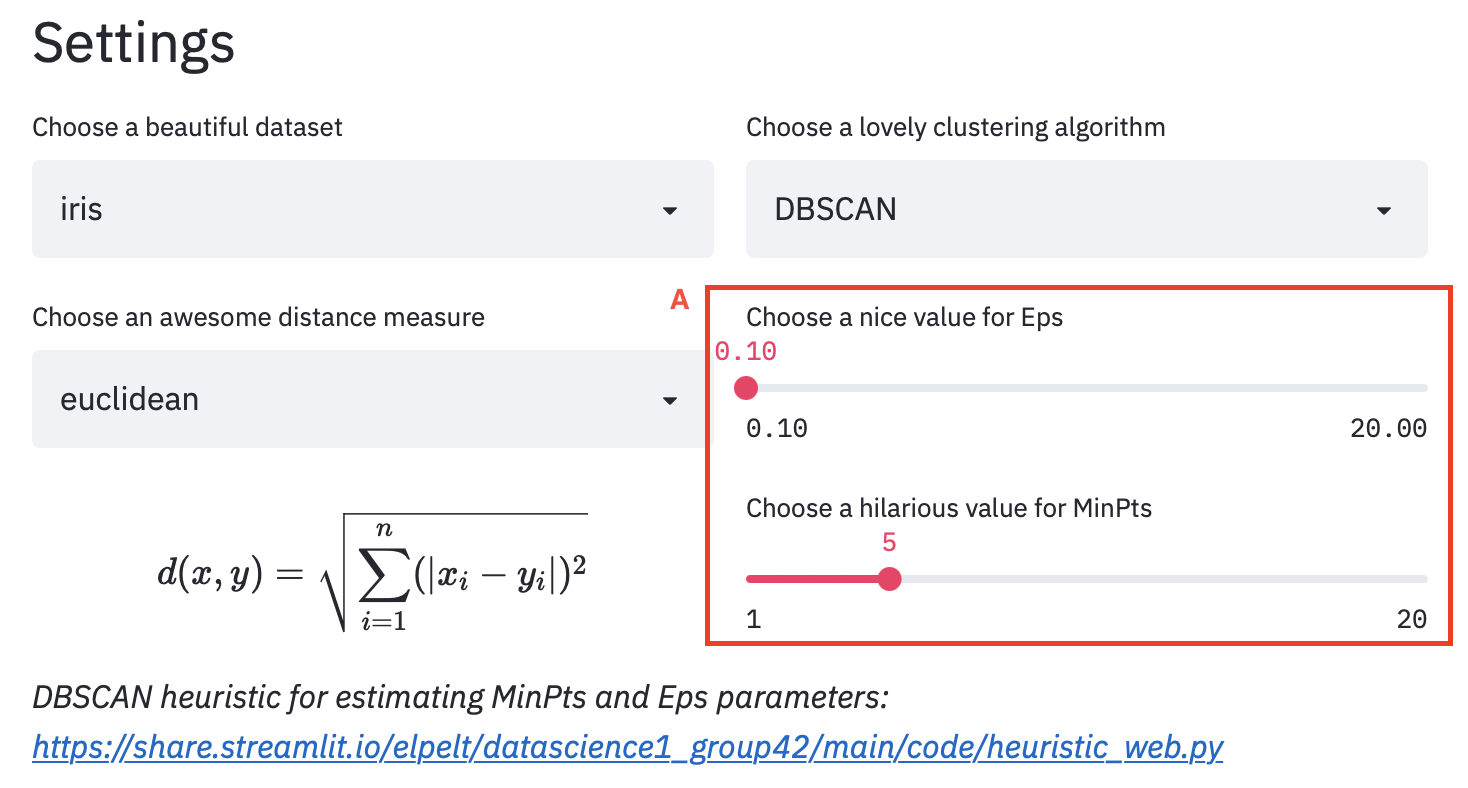
\includegraphics[width=\linewidth]{modules/web_frontend/DBSCAN_settings.png}
	\caption{Epsilon and minimal number of nearest points setting options for DBSCAN.}\label{fig:dbscan_para}
\end{figure}

For every dataset some main information can be retrieved via an expander. The dataset dimension (see \autoref{fig:data_info} A), pre classified cluster of the data (not for diabetes dataset) (see \autoref{fig:data_info} B), datatypes per column (see \autoref{fig:data_info} C), dataset preview (see \autoref{fig:data_info} D), mean per column (see \autoref{fig:data_info} E), and performed changes on the dataset are accessible (if performed).

\begin{figure}[H]
	\centering
	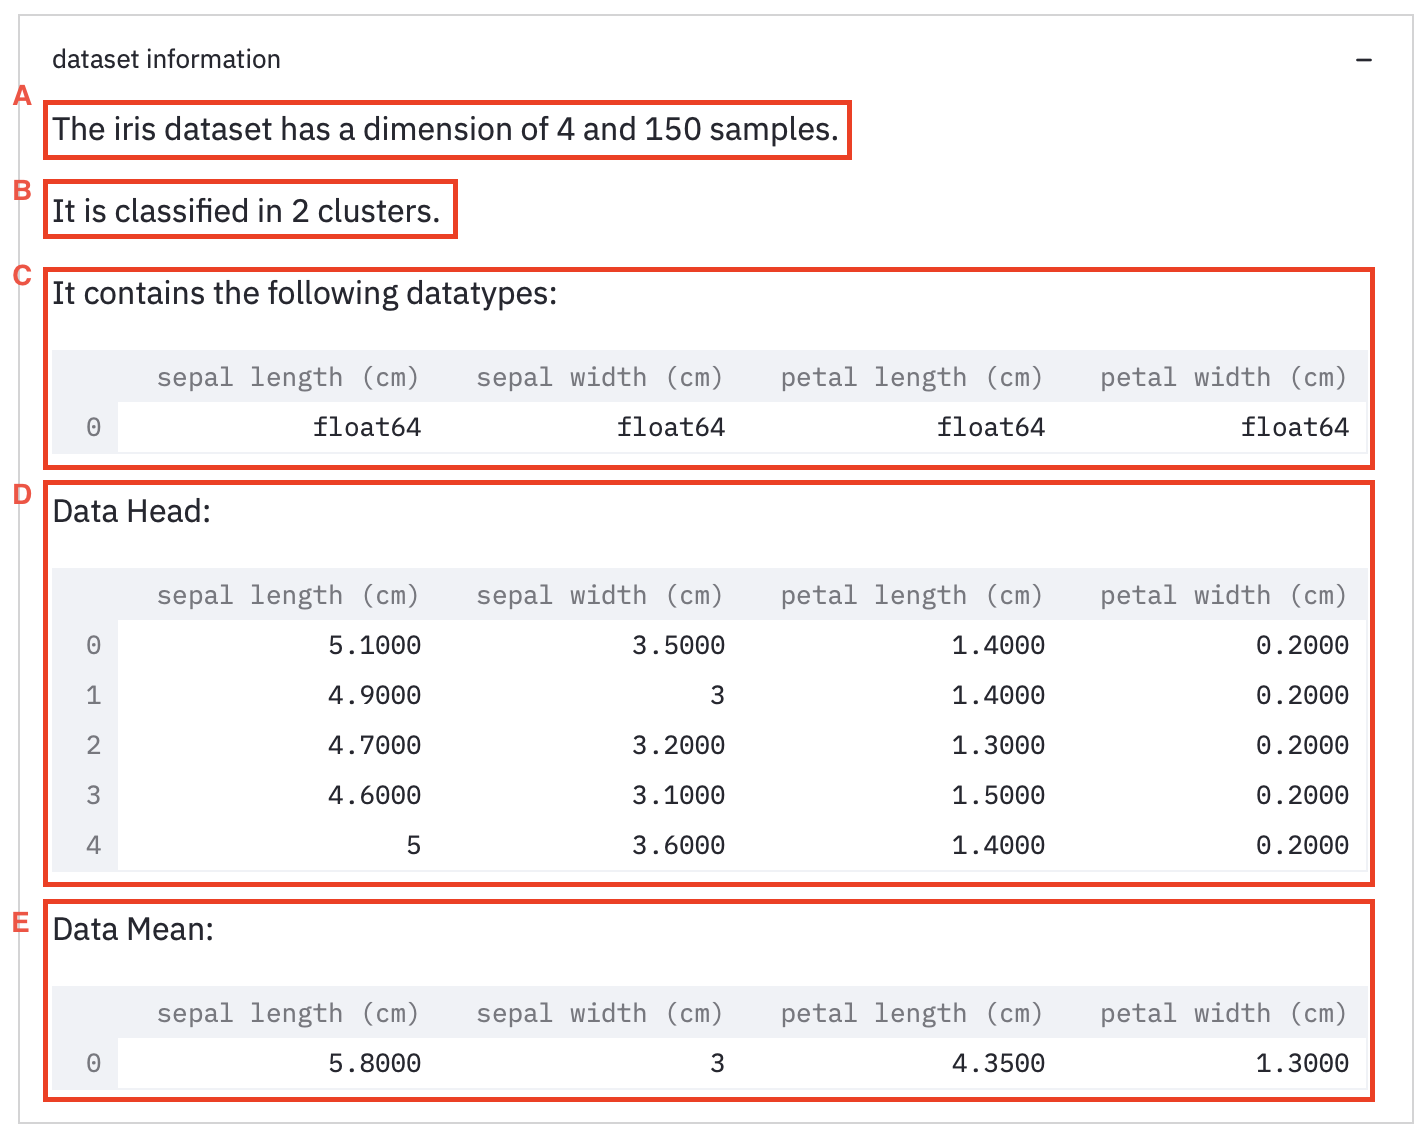
\includegraphics[width=\linewidth]{modules/web_frontend/dataset_inofs.png}
	\caption{Displayed dataset information by expanding the box by clicking on the plus. Iris dataset as example.}\label{fig:data_info}
\end{figure}

Moreover the perplexity value for the t-SNE projection can be set individually between 5 and 50 with a slider (see \autoref{fig:projection} A). The default value is 25. The \acrshort{t-SNE} and \acrshort{pca} plots are shown next to each other to allow a direct comparison of the lower-dimensional projections. For K-Medoids the medoid, for K-Means the mean, and for K-Medians the median for each cluster is marked as diamond (see \autoref{fig:projection} D). For the \acrshort{pca} plot both axis are labeled with the percentage of the first two components. To virtually interact with the plots, the button shown in \autoref{fig:projection} C can be clicked. Please note that this option is only available when the checkmark shown in \autoref{fig:parameters} B is set. Furthermore, this button provides the ability to save the plot in different formats.
The calculated runtime is displayed right under the plots (see \autoref{fig:projection} B). This info is only accessible if precalculated results are not used (see \autoref{fig:parameters} A).
The frontend is reloaded entirely if a parameter value is changed, a different setting is made or a button is clicked. 
\begin{figure}[H]
	\centering
	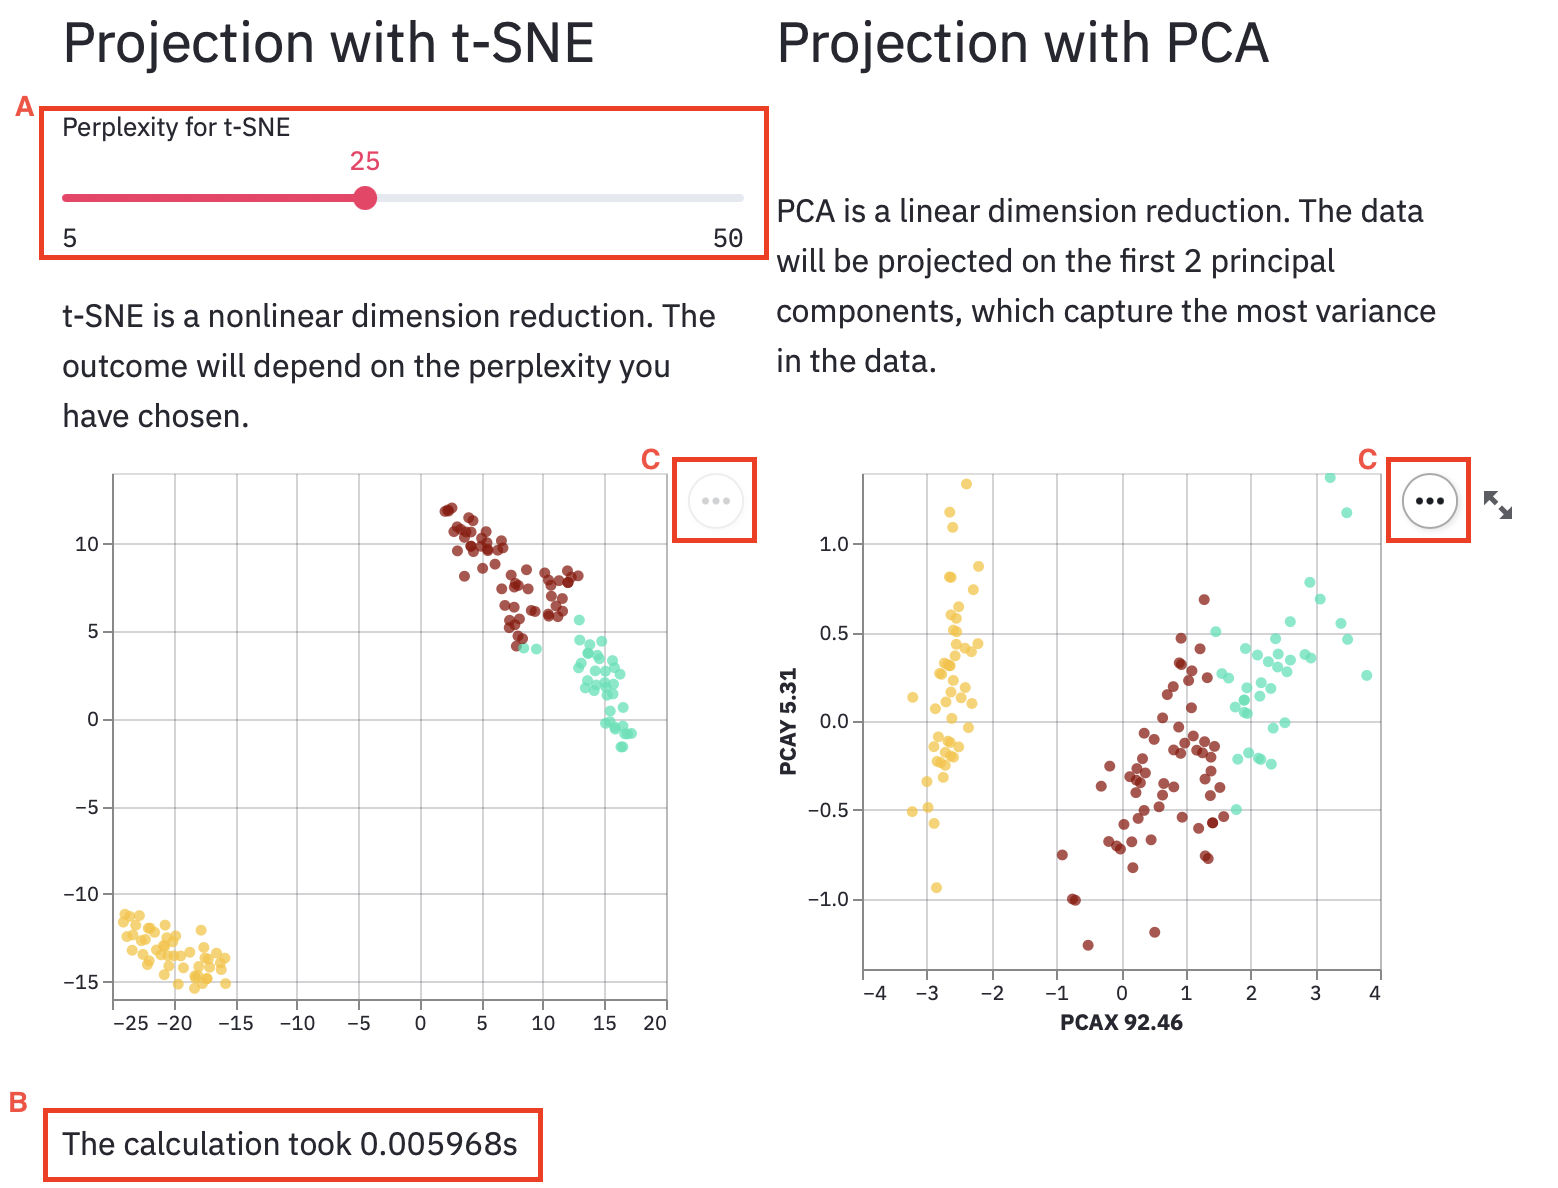
\includegraphics[width=\linewidth]{modules/web_frontend/projection_letters}
	\caption{Second part of the web frontend. Projection results of a clustering.}\label{fig:projection}
\end{figure}

The selected dataset can be viewed in a table format below the plots (see \autoref{fig:data_info_pca}).

\begin{figure}[H]
	\centering
	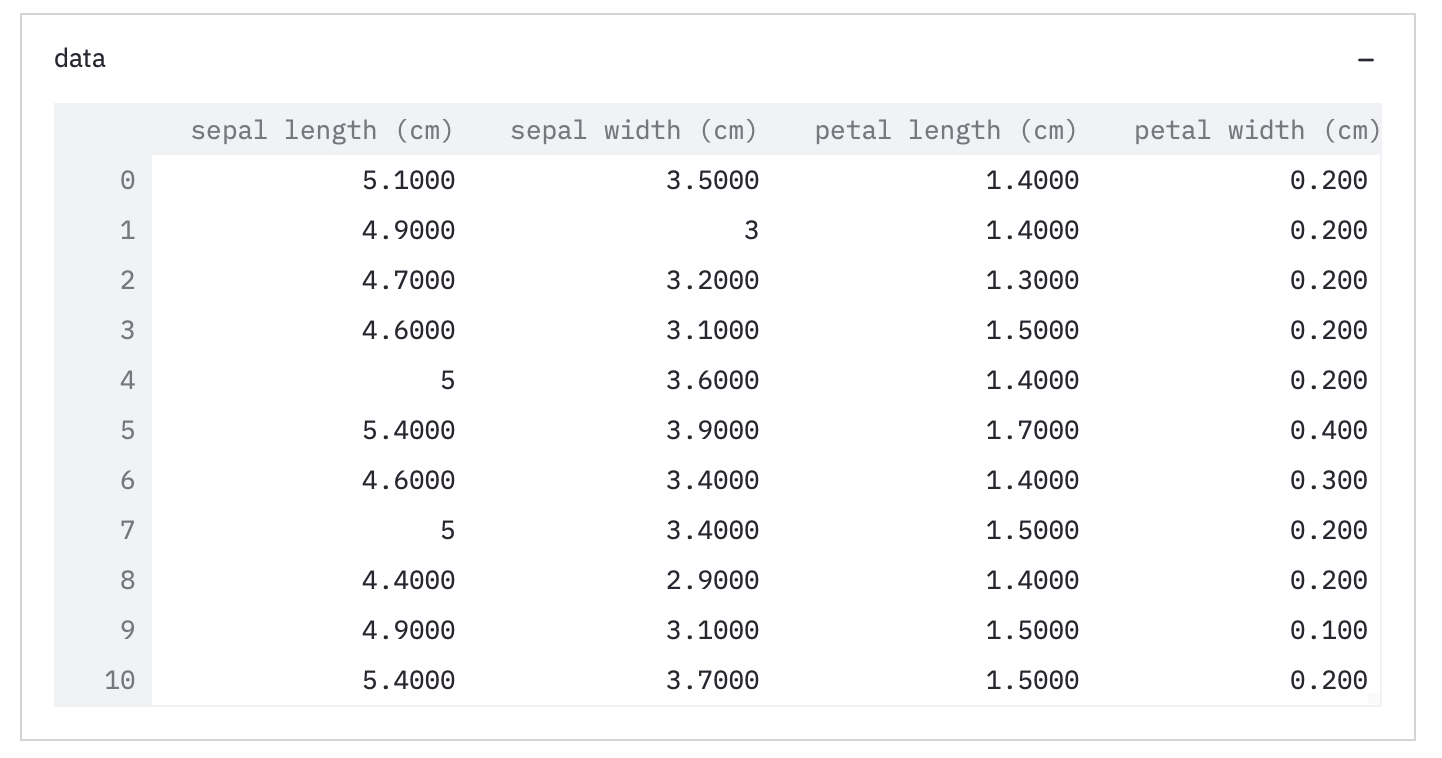
\includegraphics[width=\linewidth]{modules/web_frontend/data_info_pca.png}
	\caption{Projection of dataset as expander. Iris dataset as example.}\label{fig:data_info_pca}
\end{figure}

All clustering results can be saved in a cluster table for comparison via the \textit{Add}-button button (see \autoref{fig:evaluation} A). To compare this result to clusterings with other settings, the \textit{Add}-button can be clicked repeatedly after desired adjustment of the clustering settings. To start over and compare further clustering indices, the \textit{Reset}-button (see \autoref{fig:evaluation} B) can be clicked. The previous display of resulting indices will be cleared as well as the clustering table.
For the evaluation of the clustering results, one of five clustering indices can be chosen via a drop-down menu as shown in \autoref{fig:evaluation} C. An interactive barplot is displayed immediately, after adding a result to the cluster-table (see \autoref{fig:eval_bar}). A maximum reference value (1) is also always displayed (see \autoref{fig:eval_bar} A).
\begin{figure}[H]
	\centering
	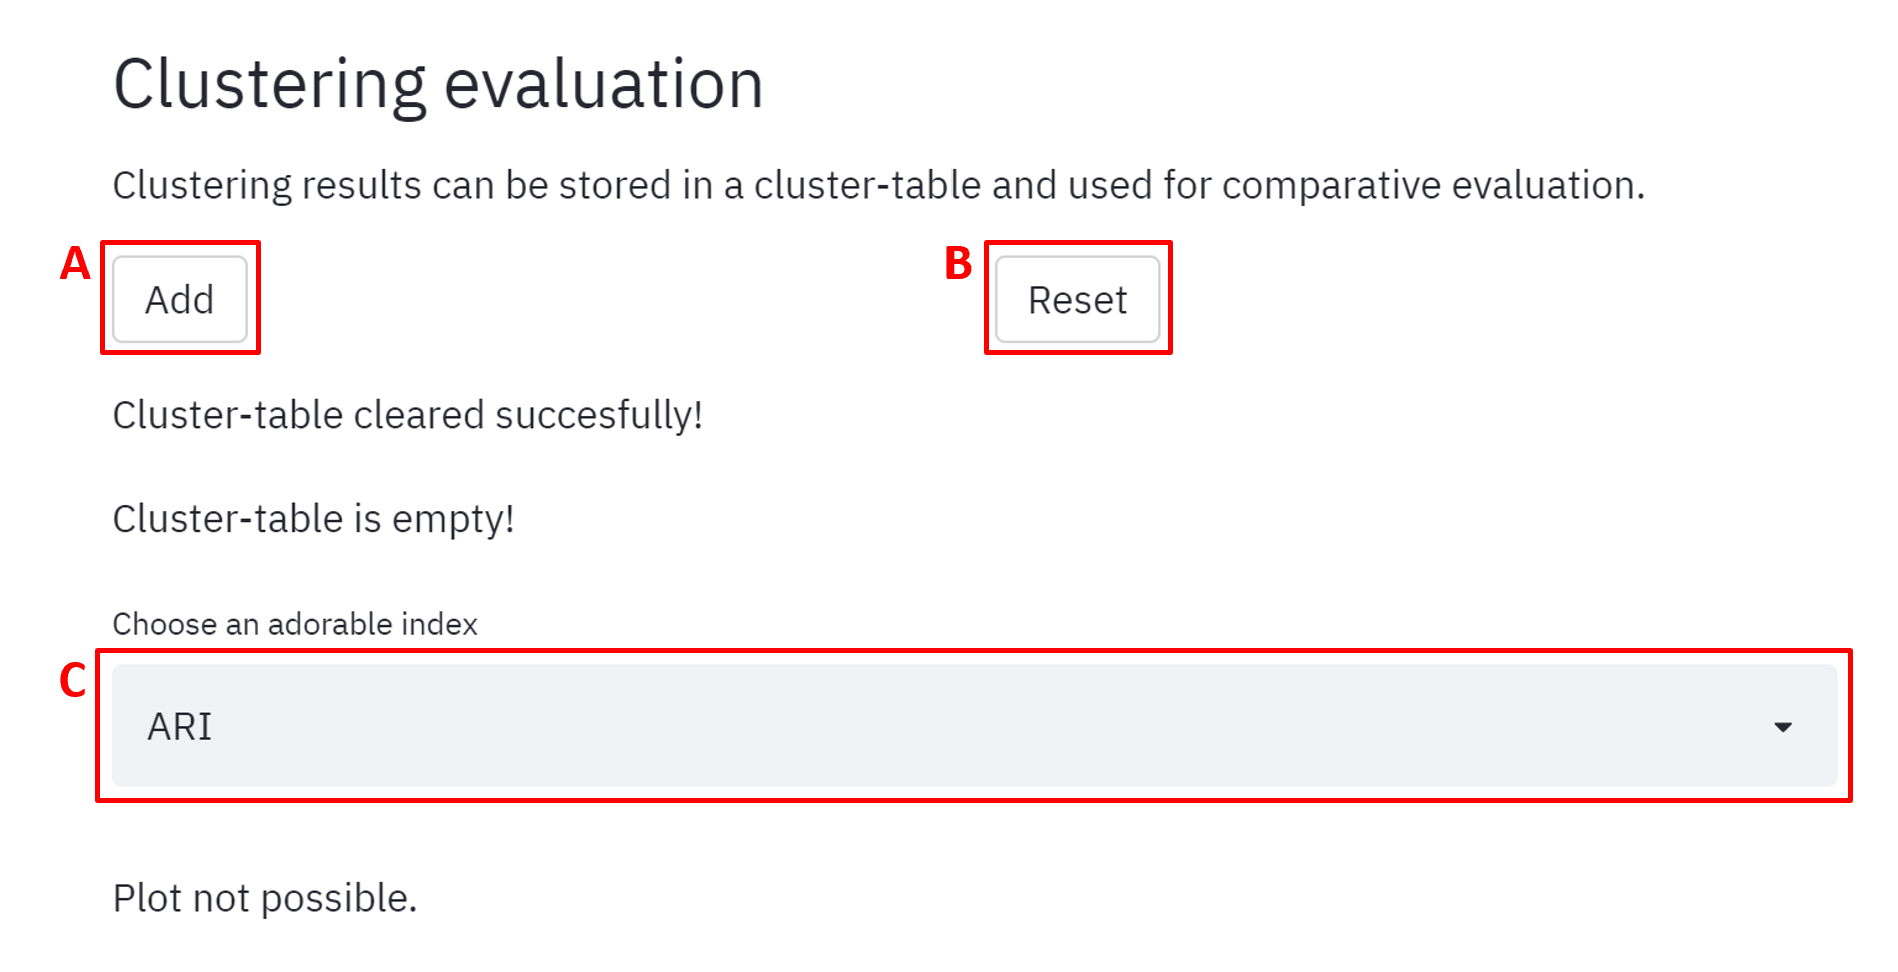
\includegraphics[width=\linewidth]{modules/web_frontend/evaluation_letters}
	\caption{Third part of the web frontend. Evaluation of clustering results.}\label{fig:evaluation}
\end{figure}

\begin{figure}[H]
	\centering
	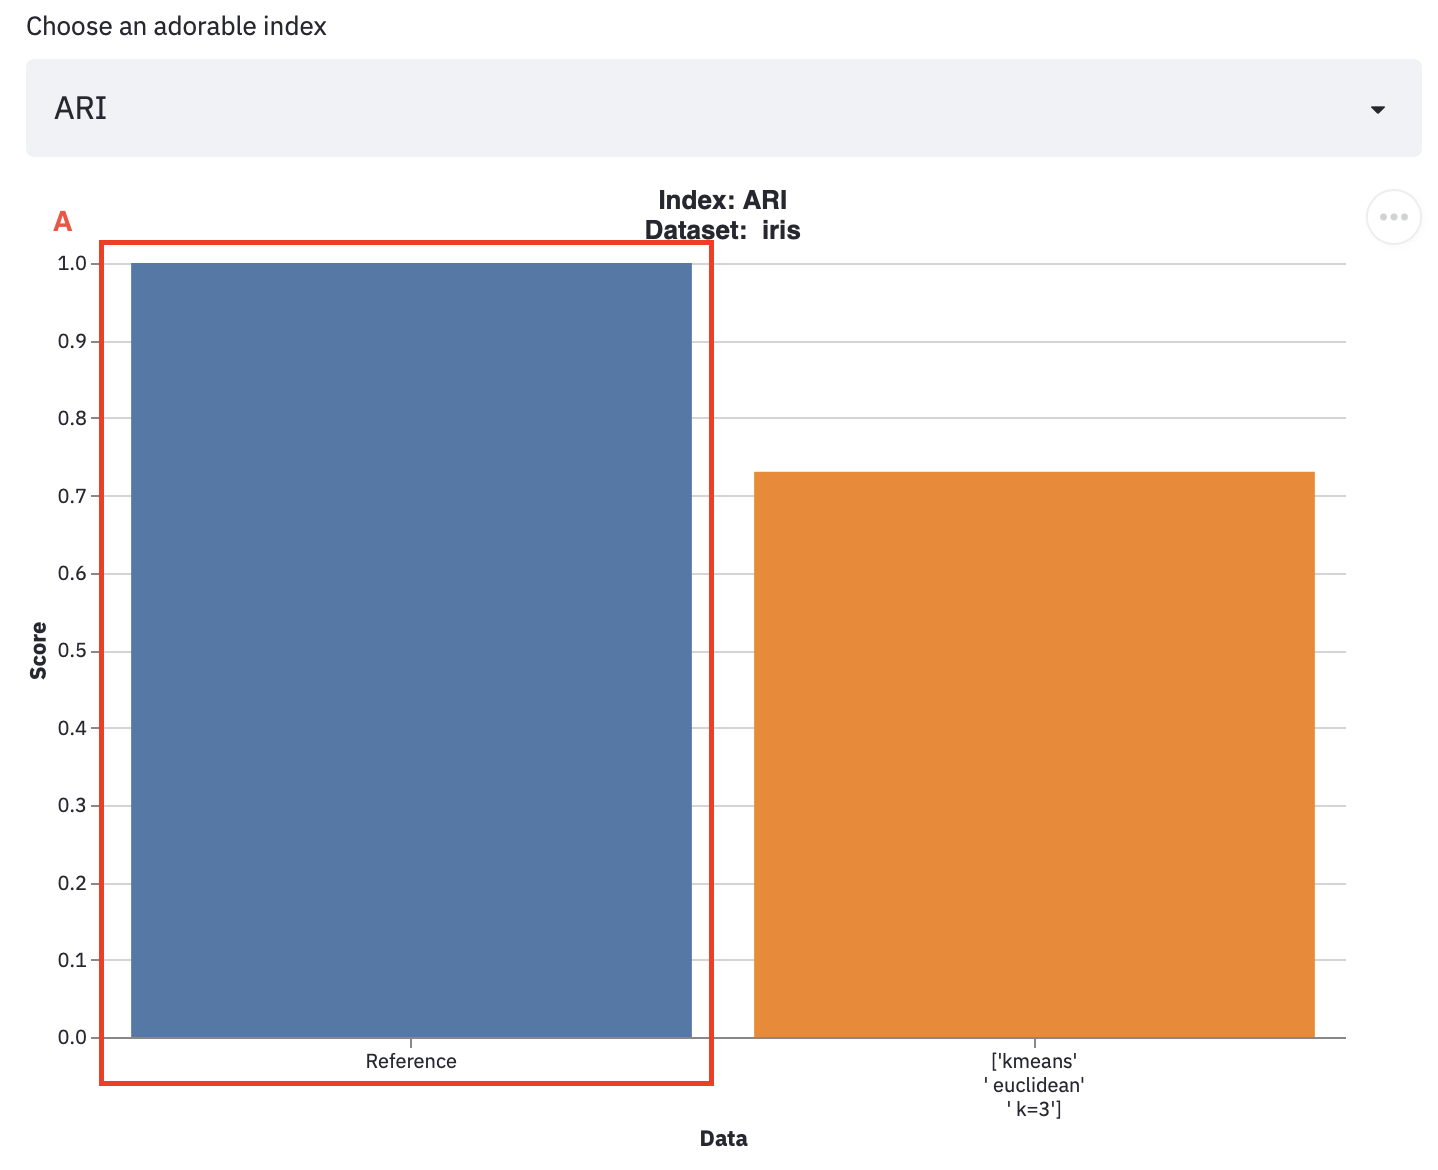
\includegraphics[width=\linewidth]{modules/web_frontend/eval_bar.png}
	\caption{Barplot for evaluation comparison. Kmeans, euclidean, k=3, iris, and \acrshort{ari} as example.}\label{fig:eval_bar}
\end{figure}

Ancillary streamlit settings can be found at the upper right corner. Additional explanatory texts provide help and more information. \\


\subsection{DBSCAN Heuristic Page} \label{heuristicmanual}
The webpage for calculating the sorted k-dist graph for the DBSCAN heuristic is build similarly to the main apps page described above.
A simple form is presented were dataset, distance measure and the k value can be chosen using drop-down menus or sliders (see \autoref{fig:evaluation} A, B, C). (Note: k in this case is not the number of clusters. k stands for the k-nearest neighbour of any point)
Only when clicking the \textit{Calculate kdist Graph}-button (see \autoref{fig:evaluation} D) the sorted k-dist graph is calculated and plotted (see \autoref{fig:evaluation} E).

\begin{figure}[H]
	\centering
	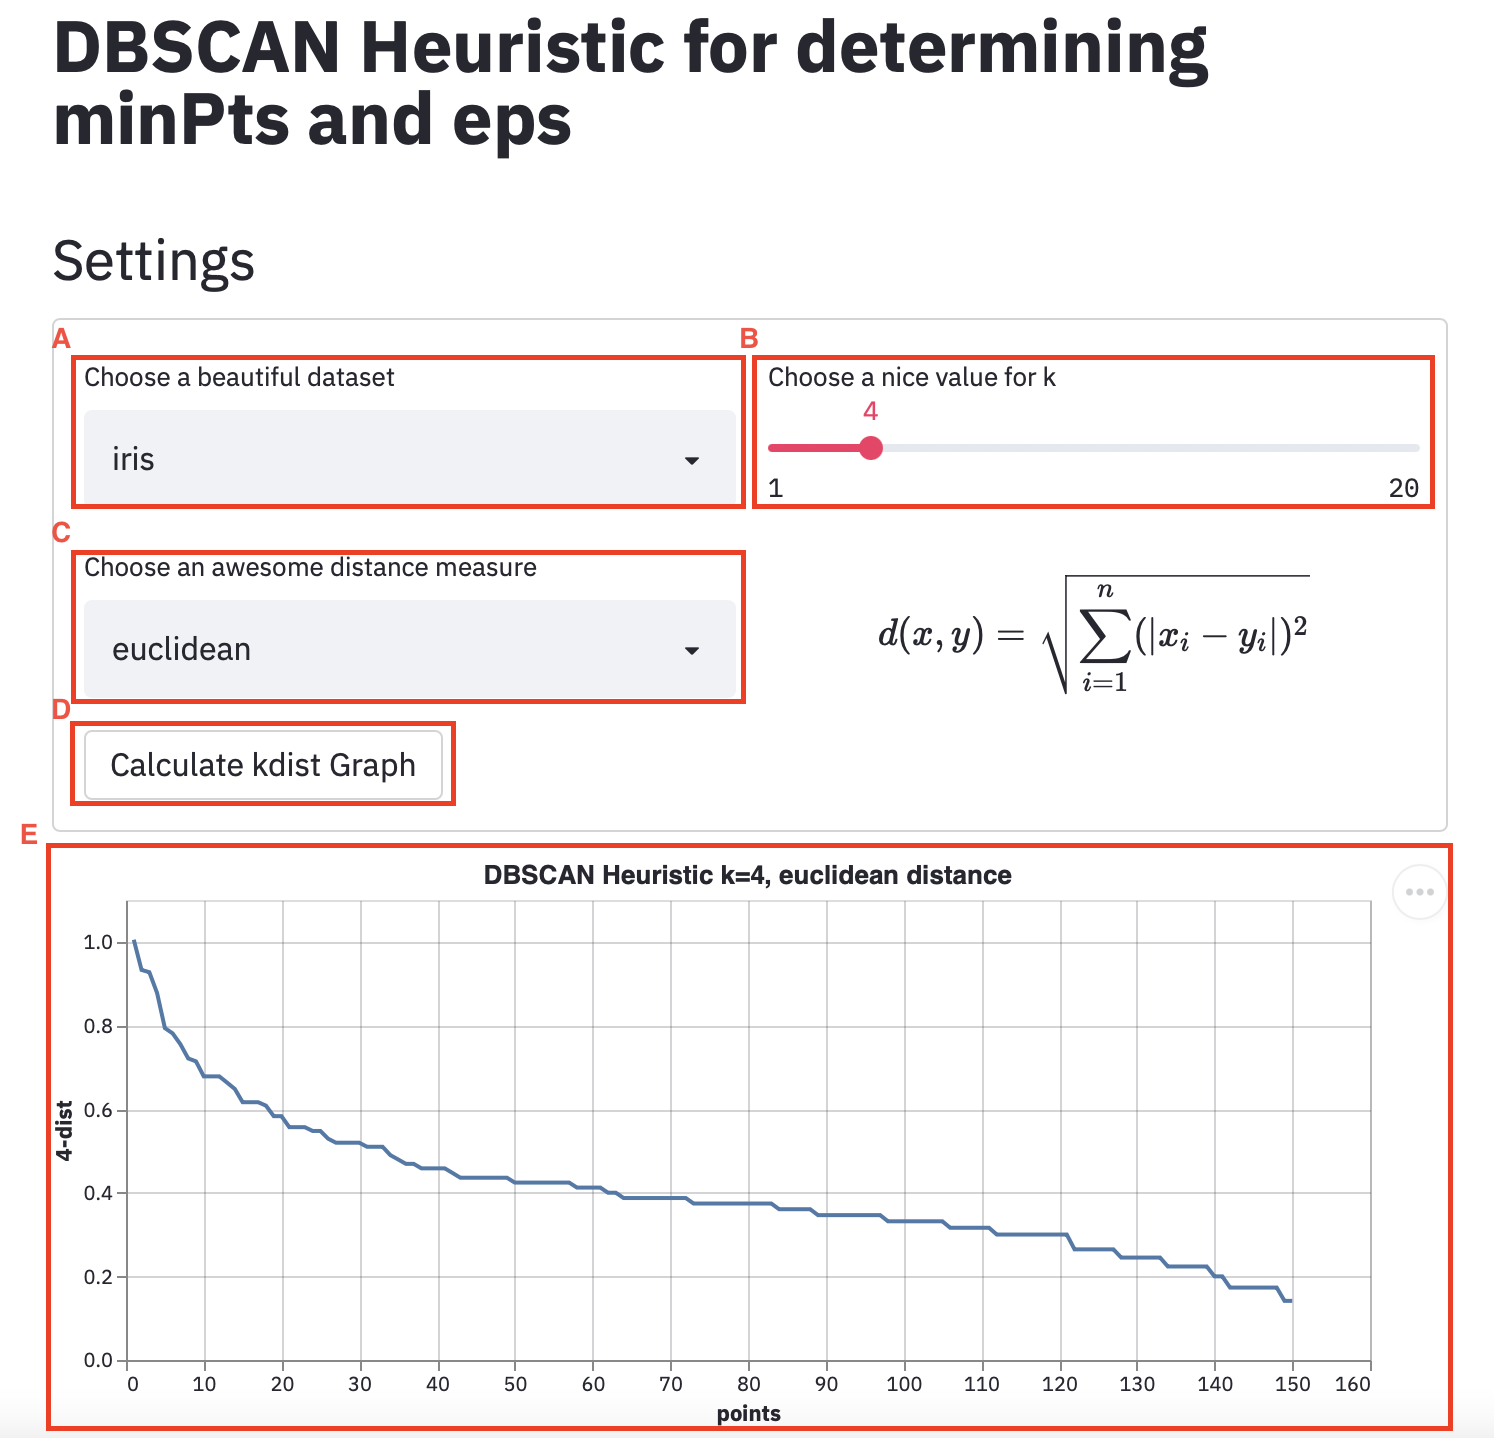
\includegraphics[width=\linewidth]{modules/web_frontend/dbscan_heuristic.png}
	\caption{DBSCAN heuristic settings}\label{fig:heuristicfrontend}
\end{figure}

\section{Conclusion}
A variety of additional algorithms, distance metrics, parameter settings and cluster evaluation measures could be considered.

We did not found a best clustering algorithm neither a superior distance measure, which would give the best results on every dataset. This problem is widely known as the "No Free Lunch Theorem" \cite{nofreelunch}. As specific requierements may differ for diverse use cases multiple algorithms and parameters should be explored and compared according to individual needs. 

\subsection{Wine Dataset}
labeled data $\rightarrow$ external validation.
k=3, because of three examined types of wine
dbscan unfit, because of distance distribution

\newpage

%print glossary
\printglossary[style=altlist,title=Glossary]
 
%print abbreviations
\printglossary[type=\acronymtype,style=long]
 
%print symbols
%\printglossary[type=symbolslist,style=long]


\newpage


\bibliography{bib.bib}
\bibliographystyle{unsrt}
\nocite{*}

\begin{appendices}
	\subsection{Comparison of different k values}

To estimate the number of meaningful clusters (clusterings with highest index scores) in the datasets and test the robustness of different distance measures we compared scorings as a function of k. \\

\begin{figure}[H]
	\centering
	\subfloat[ARI ]{{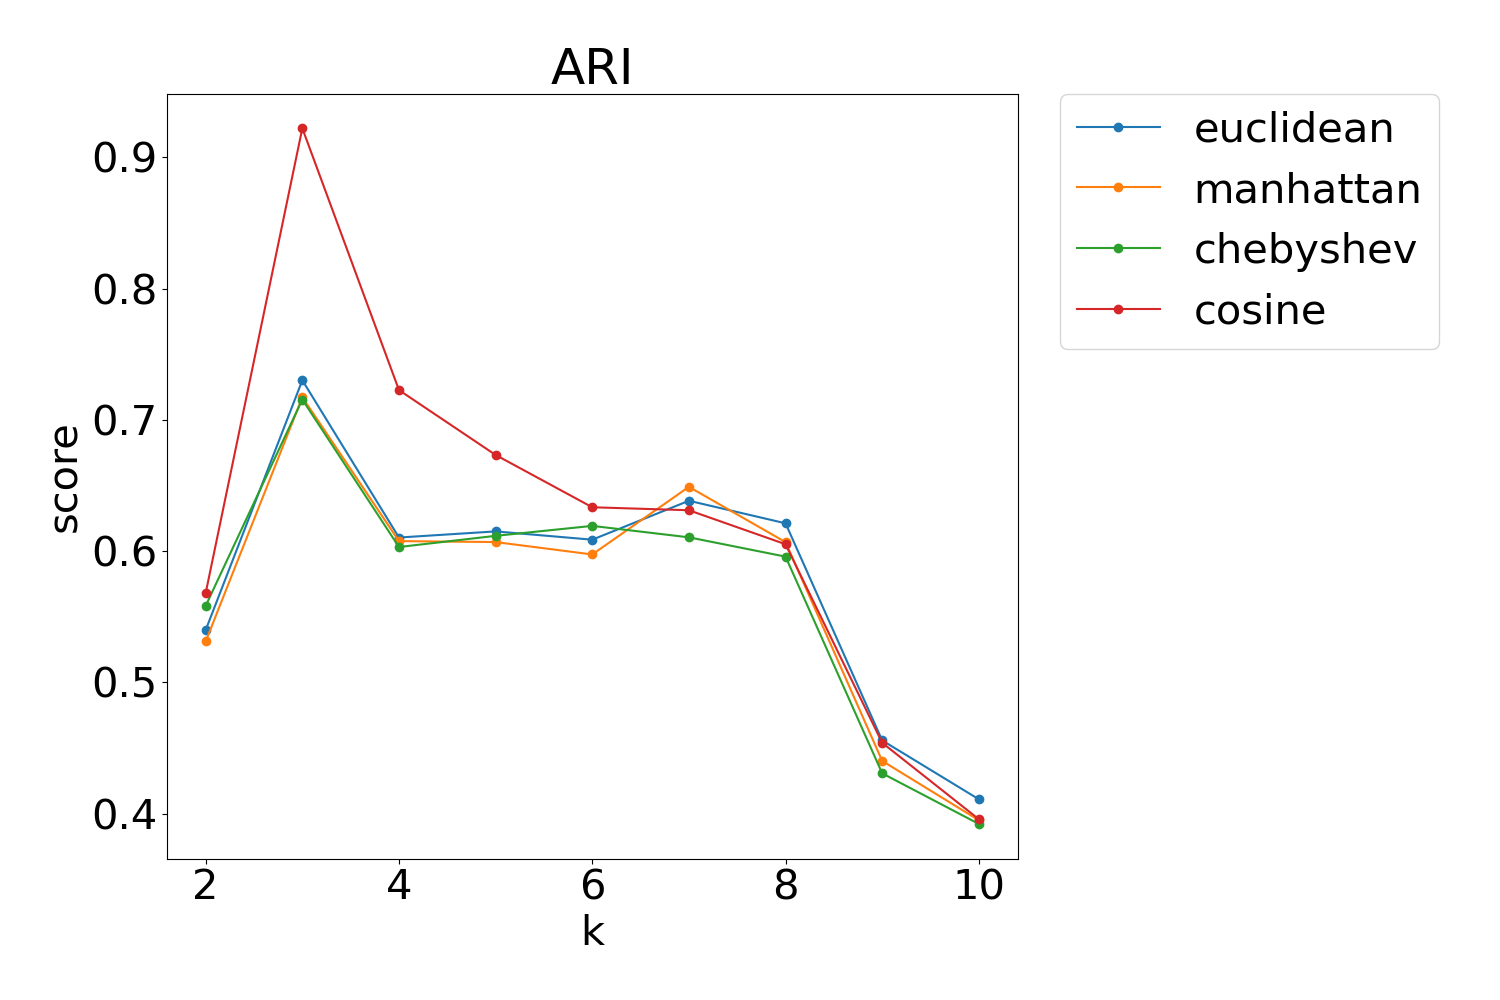
\includegraphics[width=0.45\textwidth]{../plots/iris/kmeans/ARI/k_1to10.png} }}%
	\qquad
	\subfloat[NMI ]{{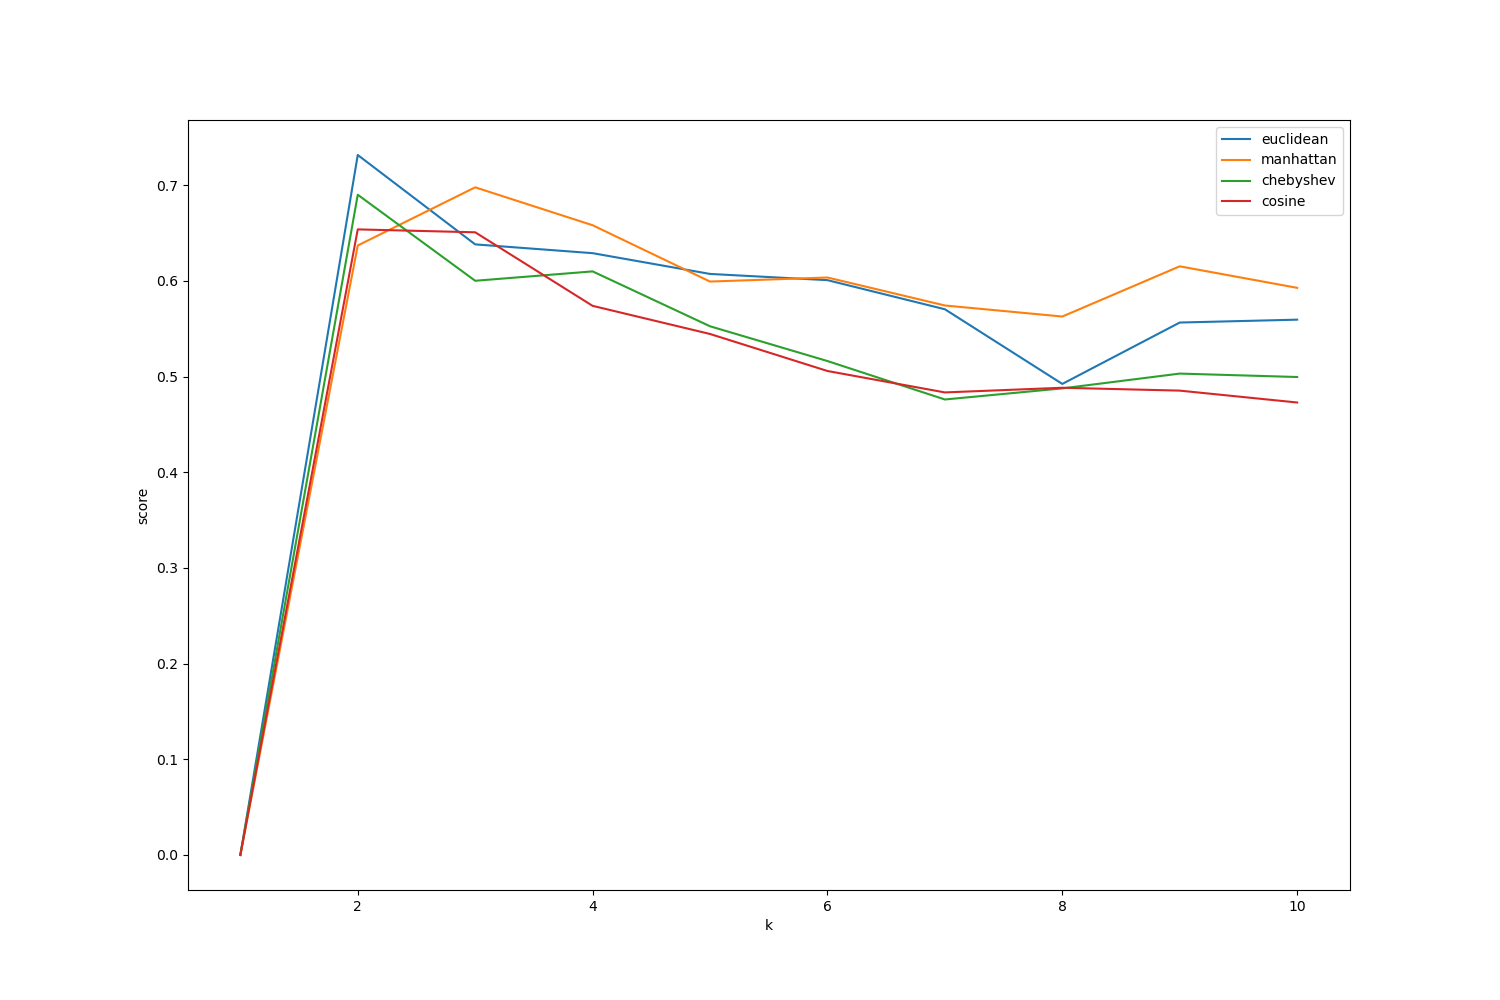
\includegraphics[width=0.45\textwidth]{../plots/iris/kmeans/NMI/k_1to10.png} }}%
	\qquad
	\subfloat[Completeness Score ]{{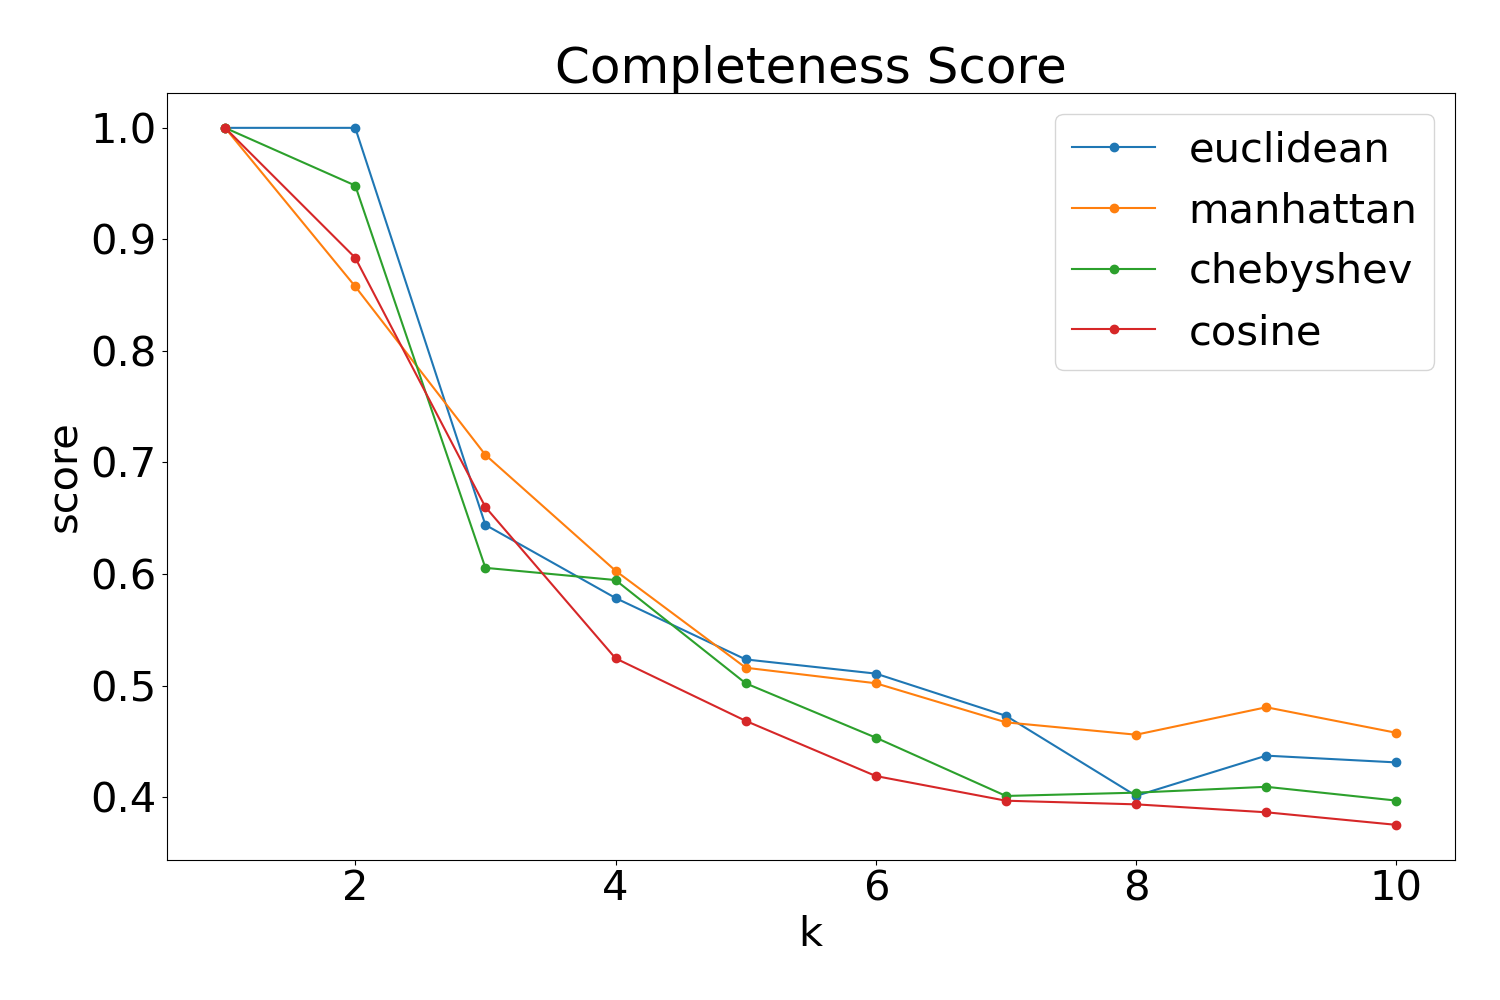
\includegraphics[width=0.45\textwidth]{../plots/iris/kmeans/Completeness Score/k_1to10.png} }}%
	\qquad
	\subfloat[Homogeneity Score ]{{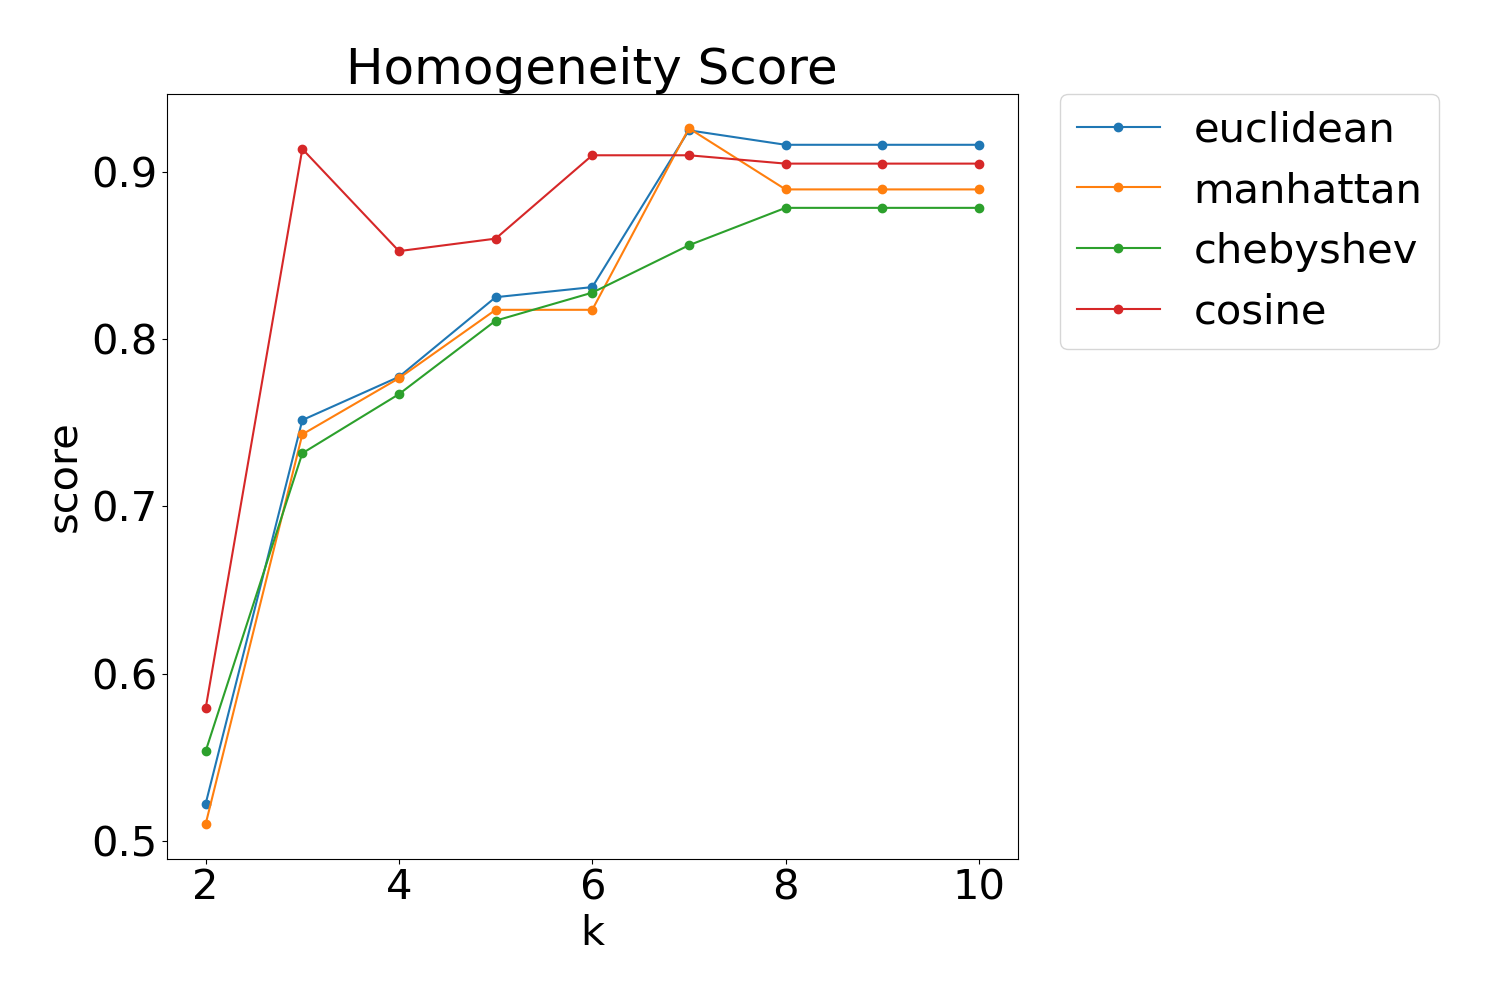
\includegraphics[width=0.45\textwidth]{../plots/iris/kmeans/Homogeneity Score/k_1to10.png} }}%
	\qquad
	\subfloat[Silhouette Score ]{{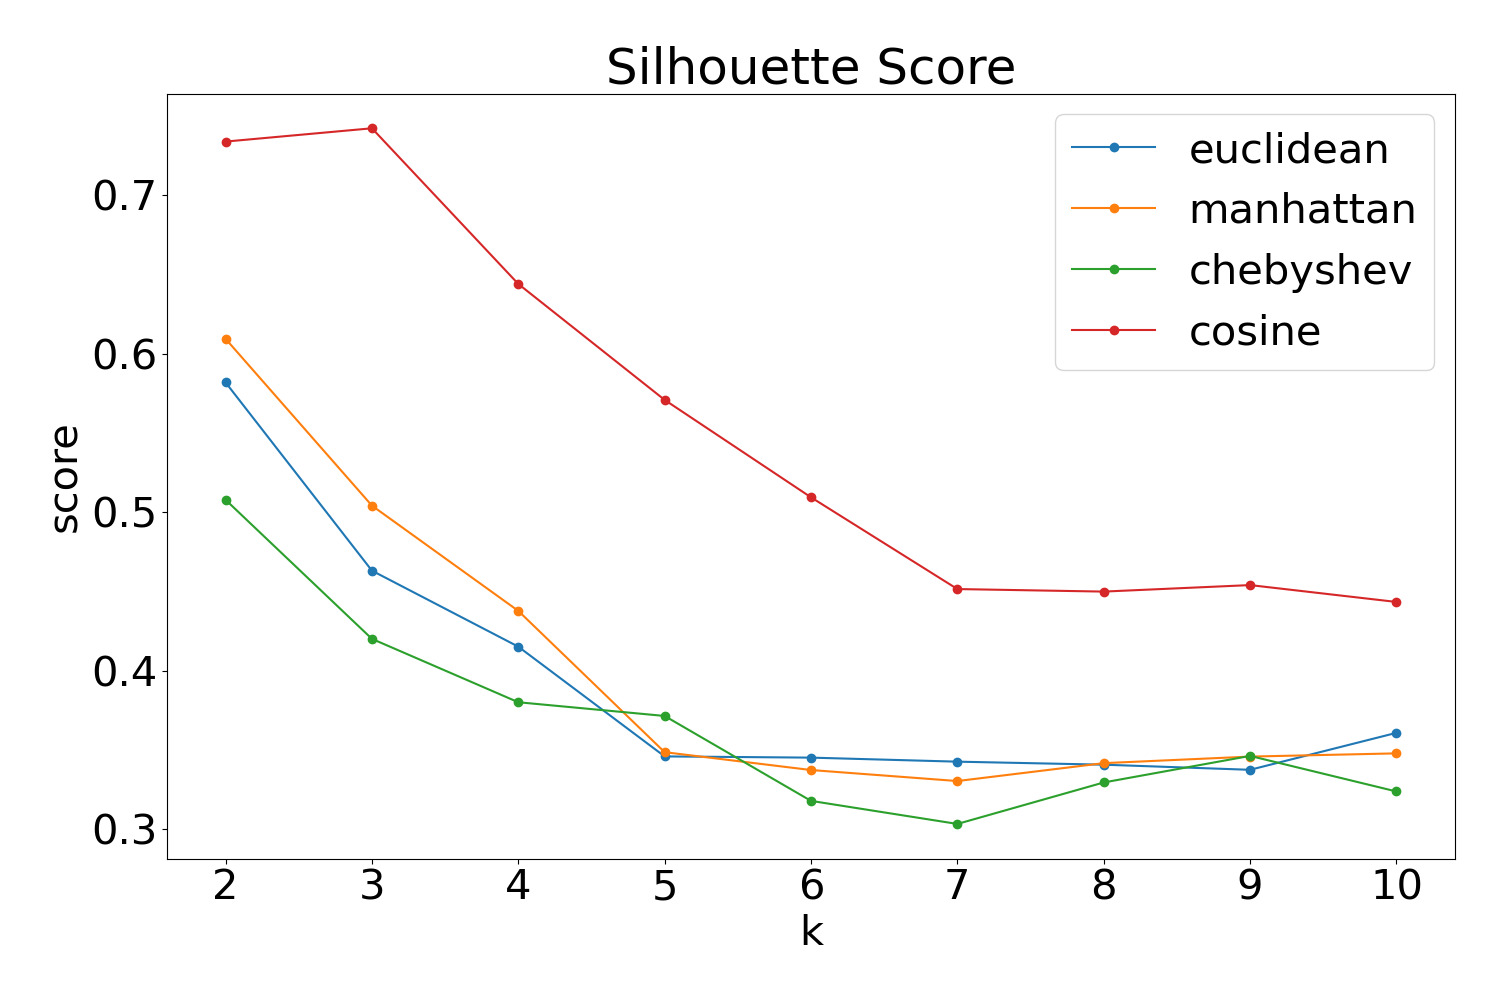
\includegraphics[width=1\textwidth]{../plots/iris/kmeans/Silhouette Score/k_1to10.png} }}%
	
	\caption{Comparison of clustering scores for kmeans-clustering on Iris dataset}%
\end{figure}

\begin{figure}[H]
	\centering
	\subfloat[ARI ]{{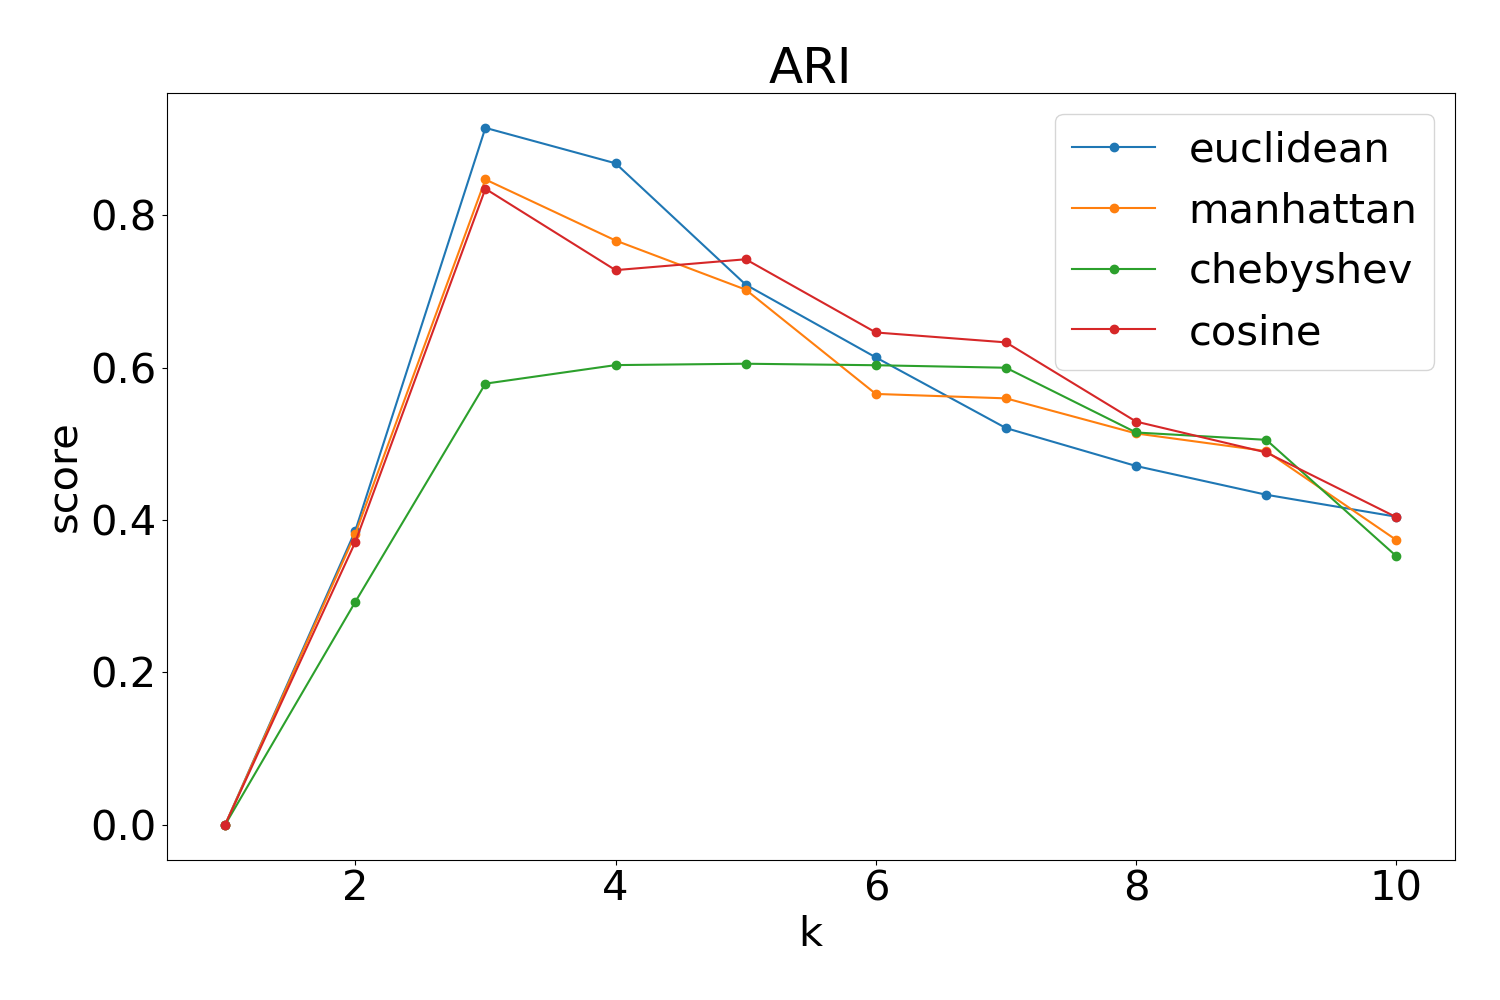
\includegraphics[width=0.45\textwidth]{../plots/wine/kmeans/ARI/k_1to10.png} }}%
	\qquad
	\subfloat[NMI ]{{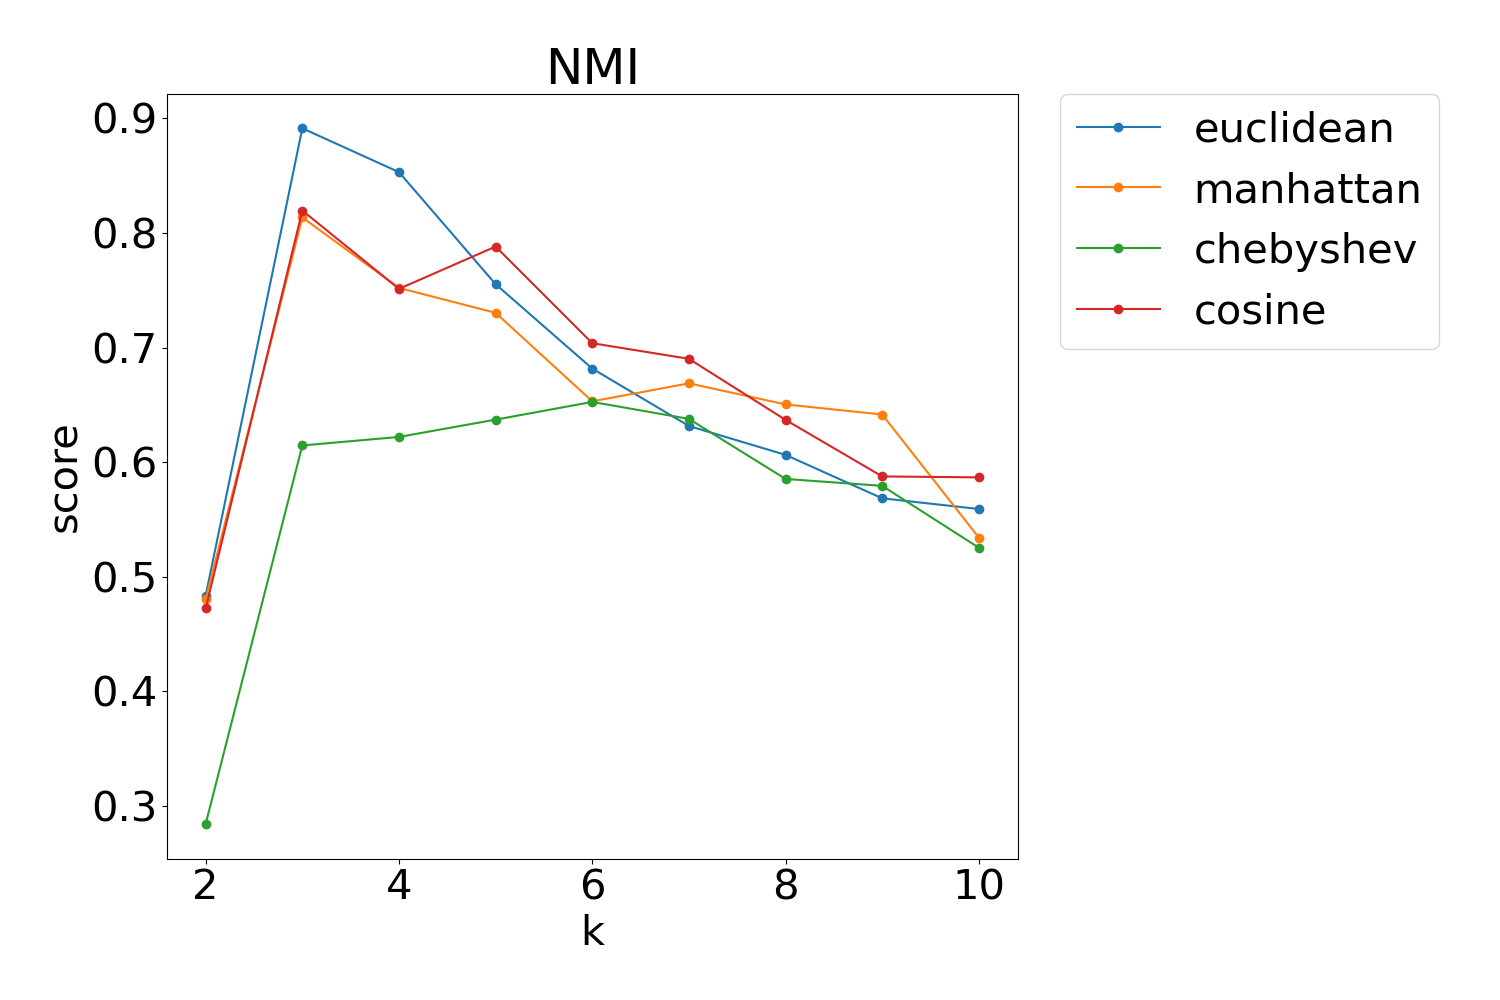
\includegraphics[width=0.45\textwidth]{../plots/wine/kmeans/NMI/k_1to10.png} }}%
	\qquad
	\subfloat[Completeness Score ]{{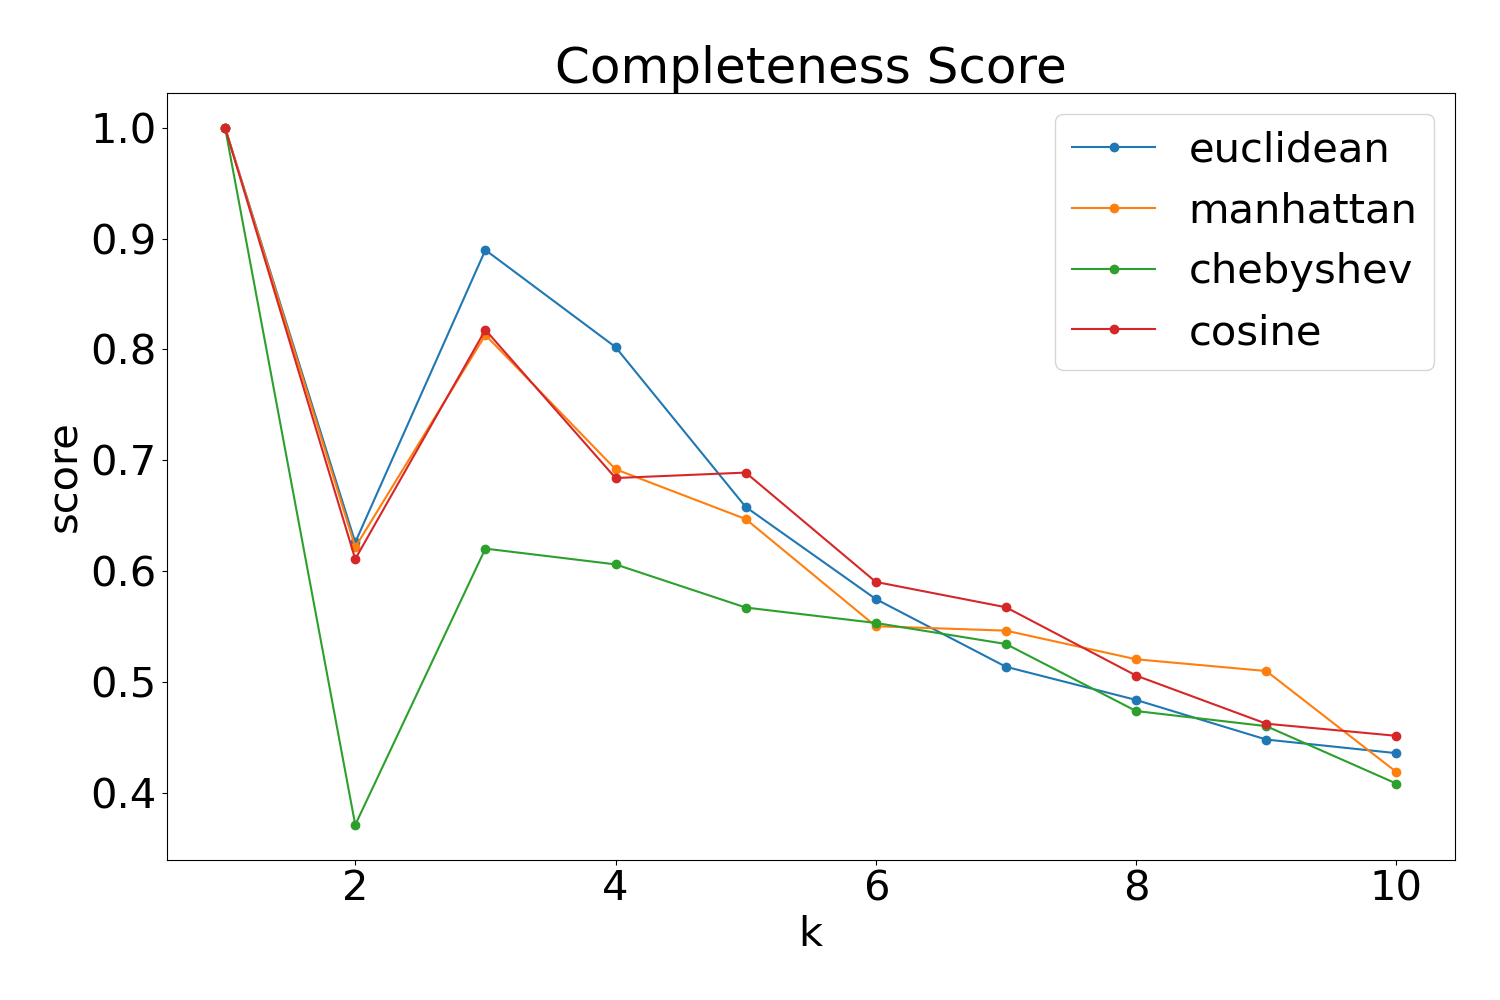
\includegraphics[width=0.45\textwidth]{../plots/wine/kmeans/Completeness Score/k_1to10.png} }}%
	\qquad
	\subfloat[Homogeneity Score ]{{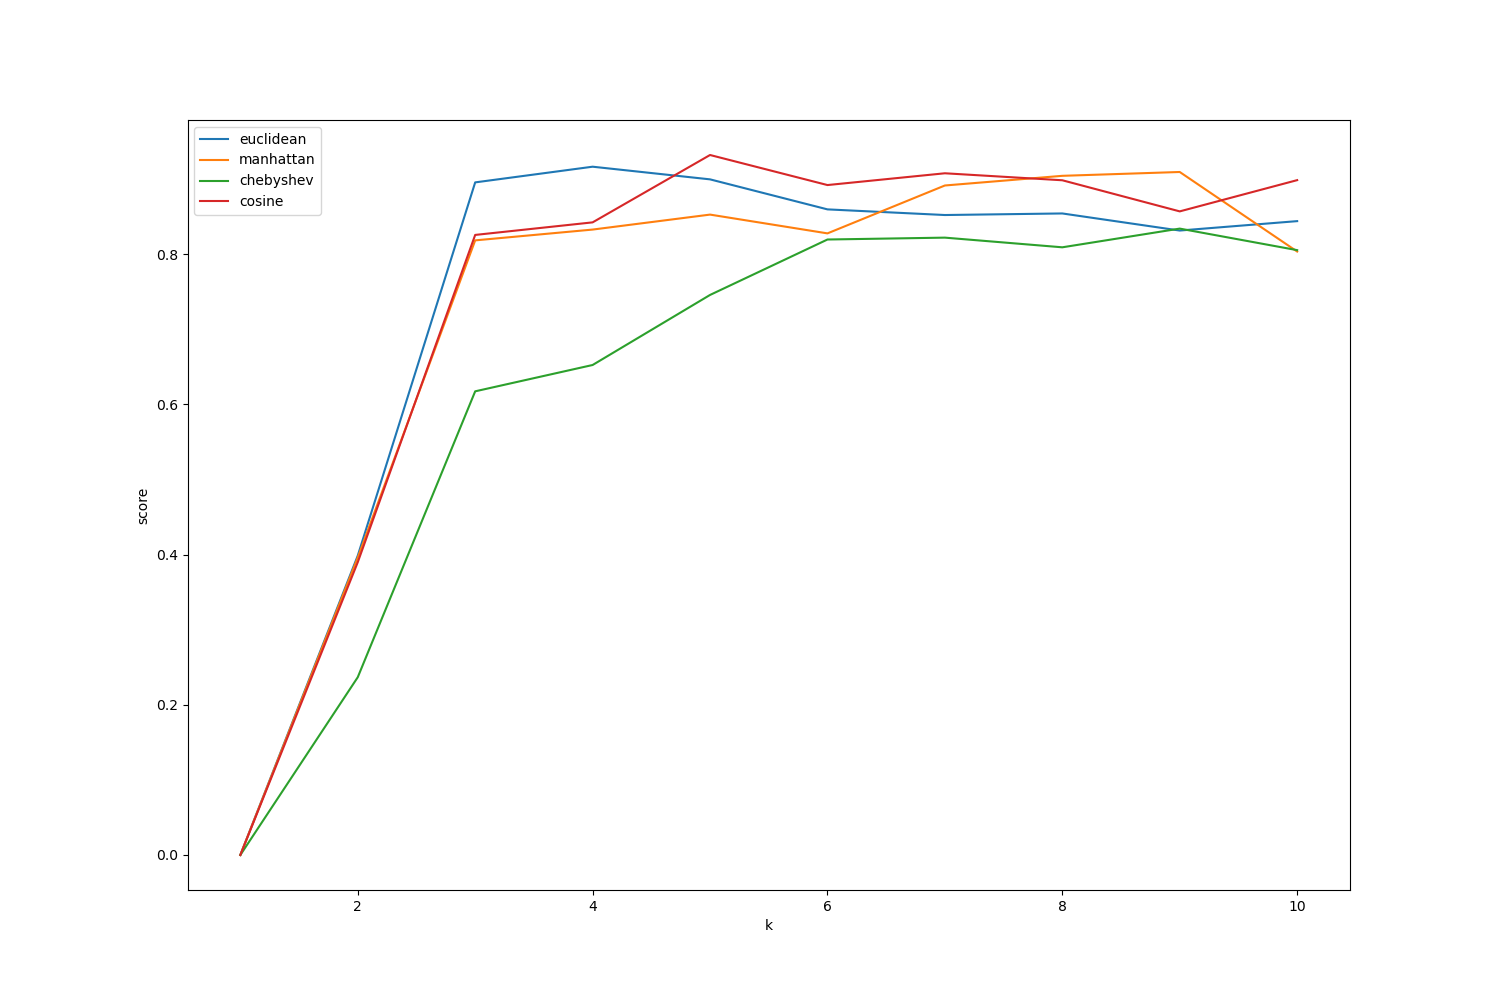
\includegraphics[width=0.45\textwidth]{../plots/wine/kmeans/Homogeneity Score/k_1to10.png} }}%
	\qquad
	\subfloat[Silhouette Score ]{{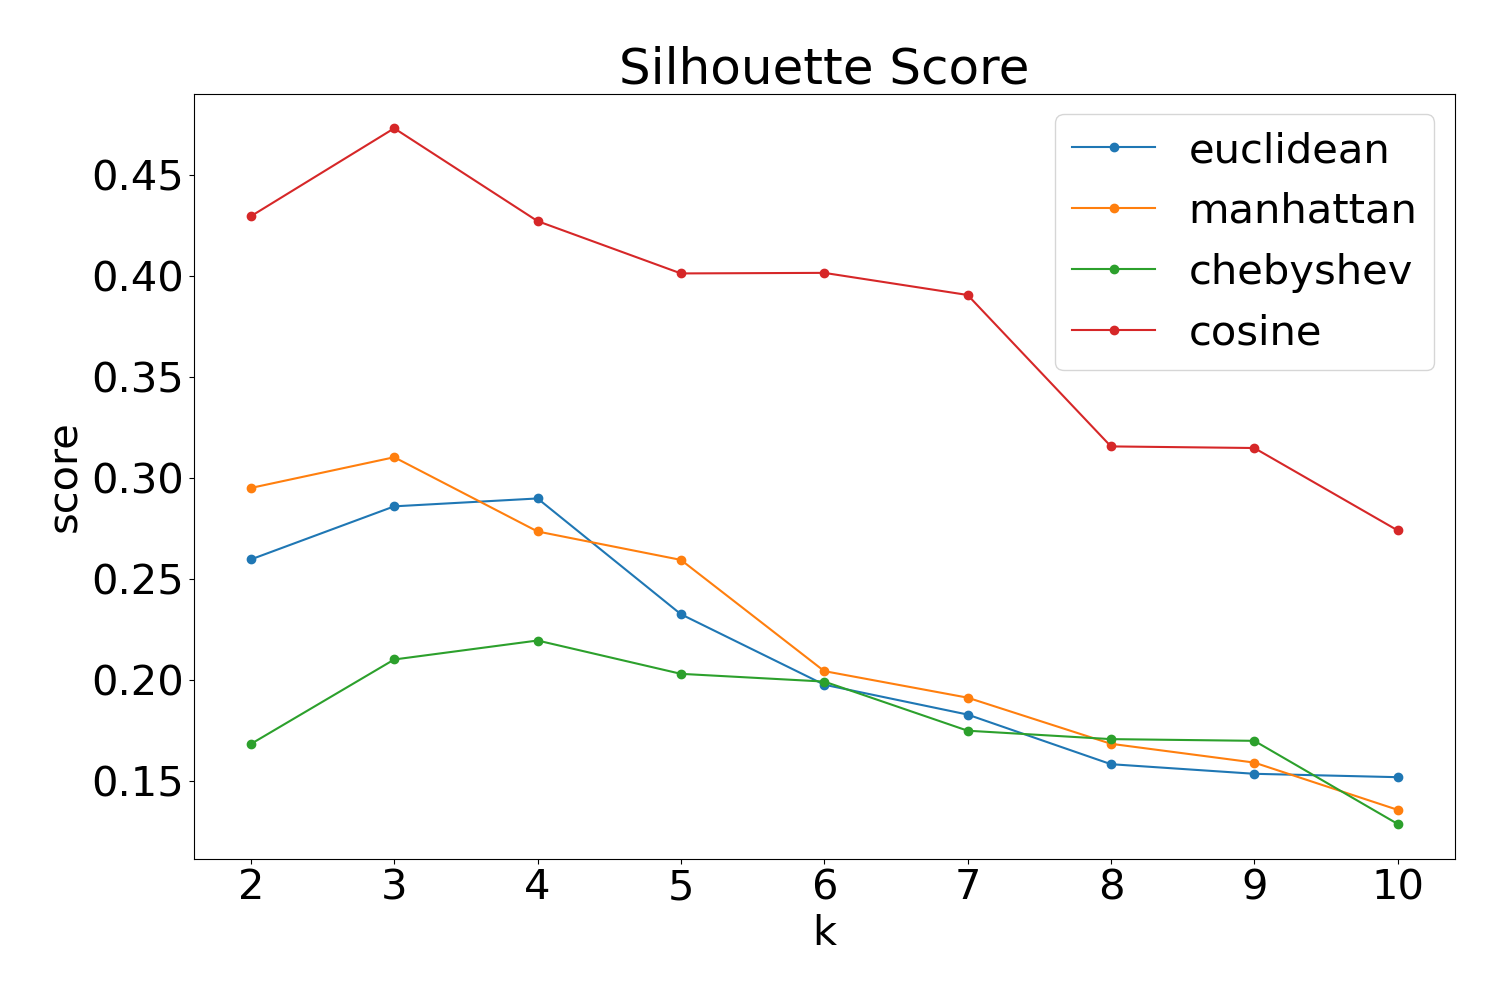
\includegraphics[width=1\textwidth]{../plots/wine/kmeans/Silhouette Score/k_1to10.png} }}%
	
	\caption{Comparison of clustering scores for kmeans-clustering on Wine dataset}%
\end{figure}

\begin{figure}[H]
	\centering
	\subfloat[Silhouette Score ]{{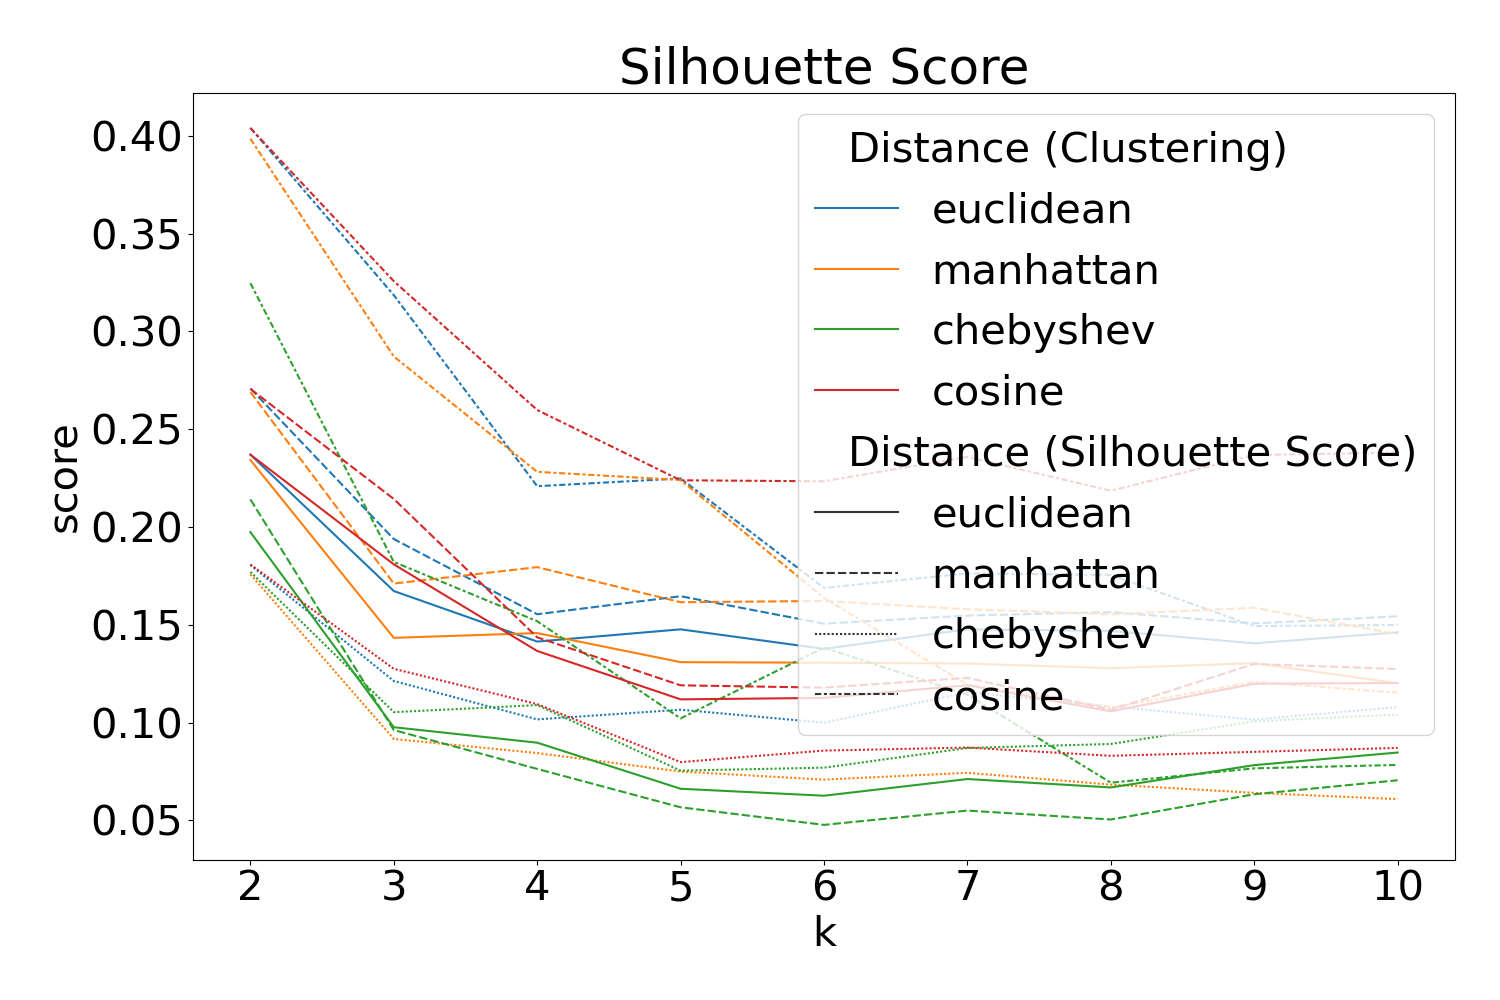
\includegraphics[width=1\textwidth]{../plots/diabetes/kmeans/Silhouette Score/k_1to10.png} }}%
	
	\caption{Comparison of clustering scores for kmeans-clustering on Diabetes dataset}%
\end{figure}

\begin{figure}[H]
	\centering
	\subfloat[ARI ]{{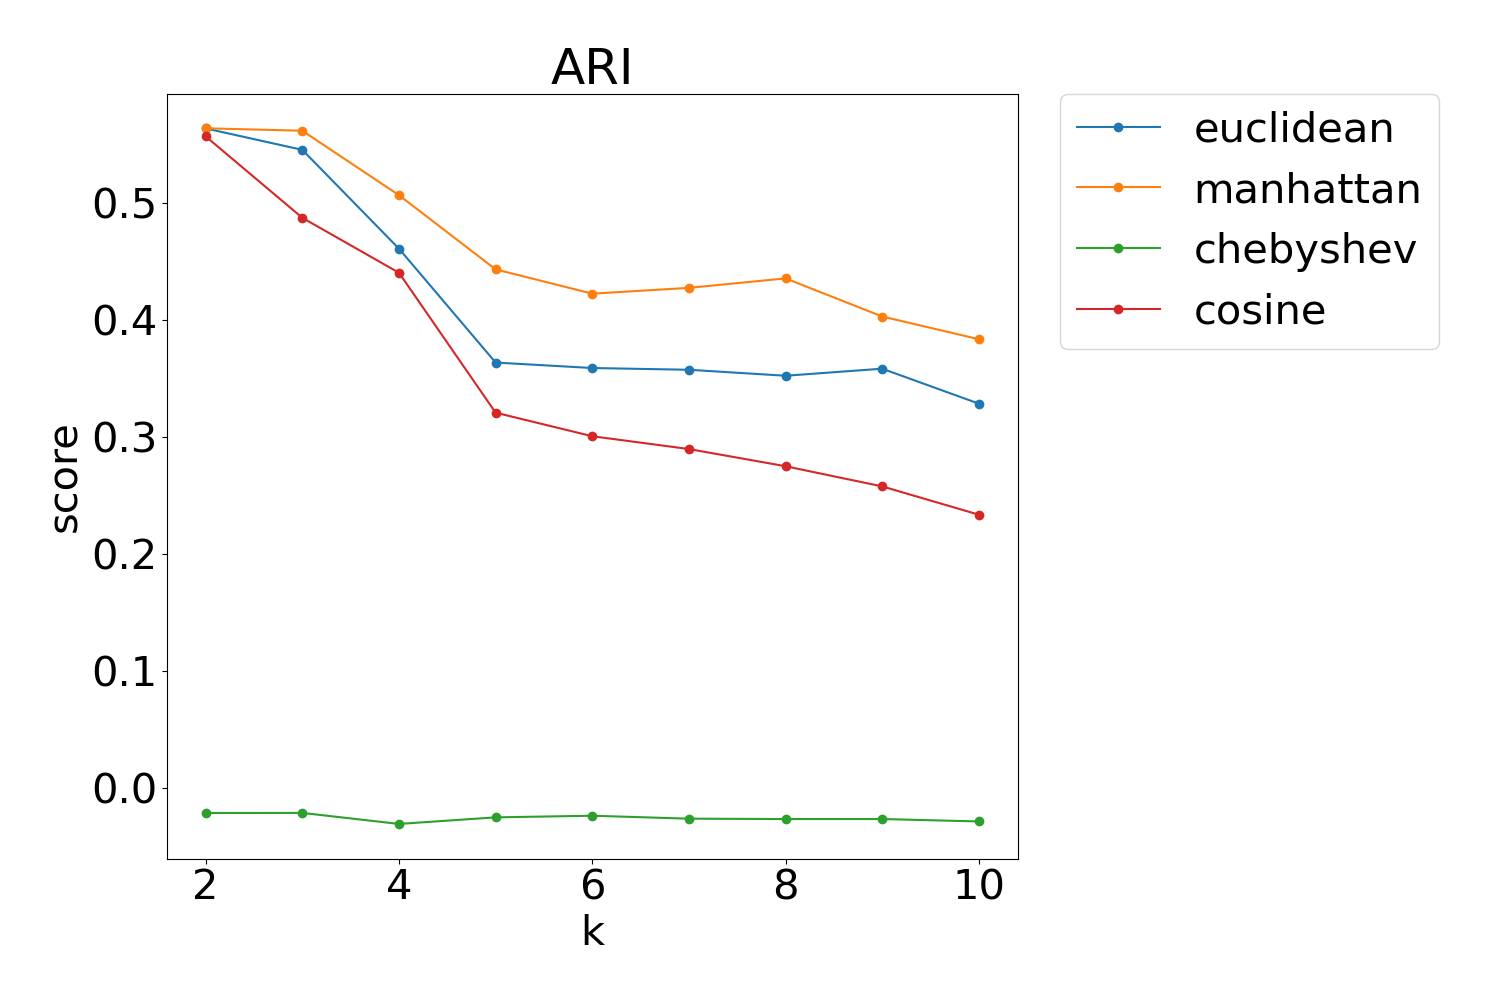
\includegraphics[width=0.45\textwidth]{../plots/housevotes/kmeans/ARI/k_1to10.png} }}%
	\qquad
	\subfloat[NMI ]{{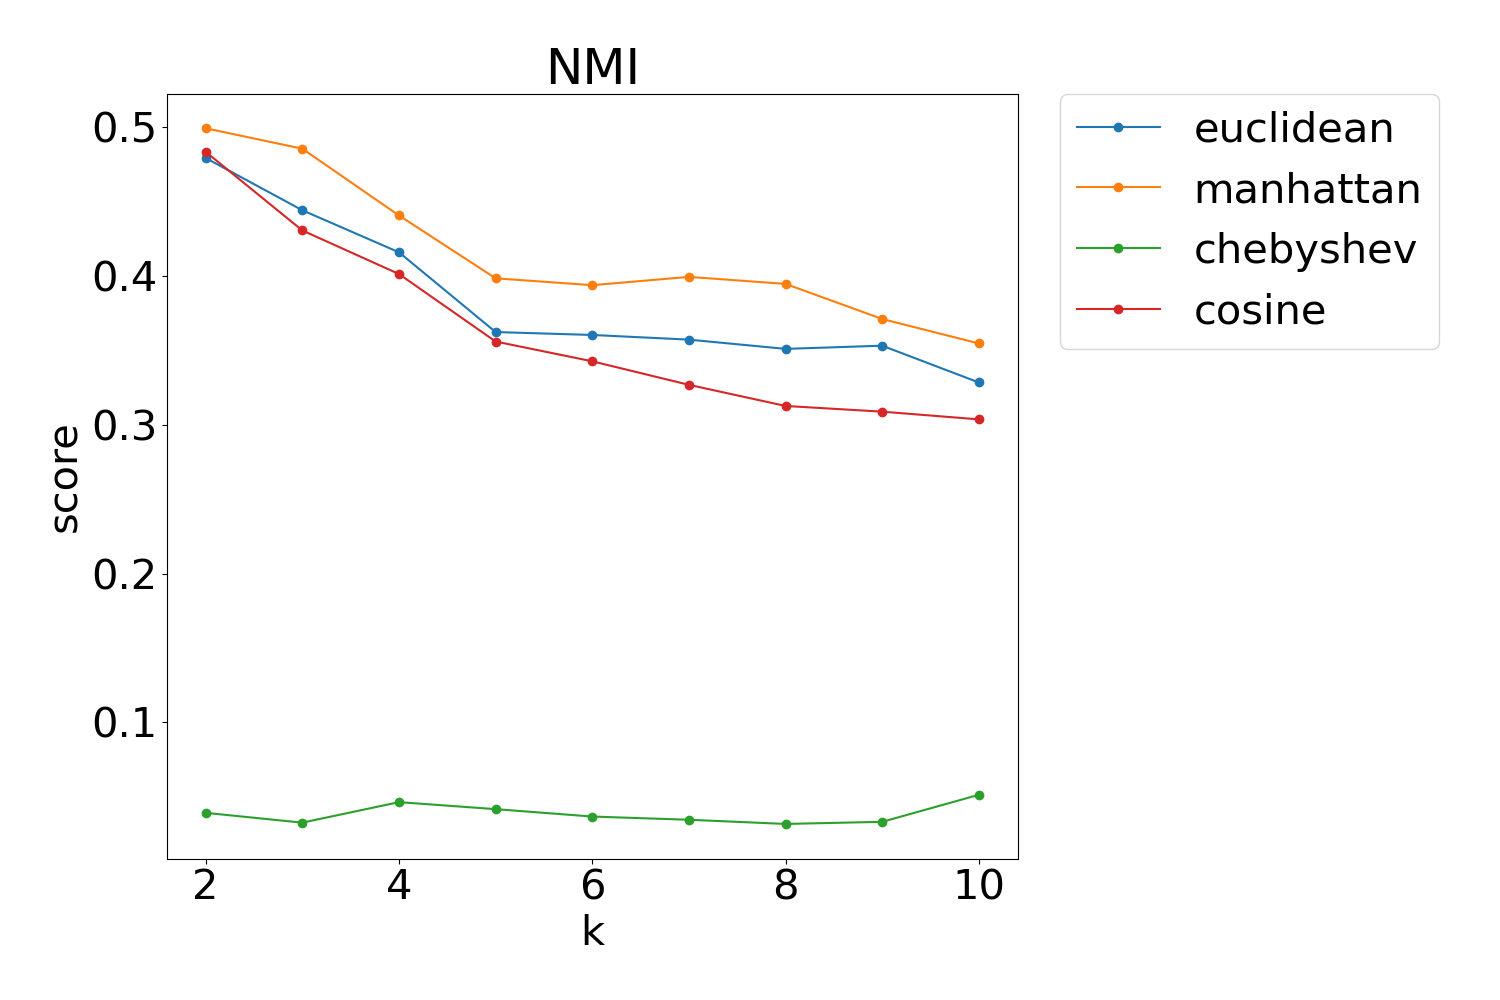
\includegraphics[width=0.45\textwidth]{../plots/housevotes/kmeans/NMI/k_1to10.png} }}%
	\qquad
	\subfloat[Completeness Score ]{{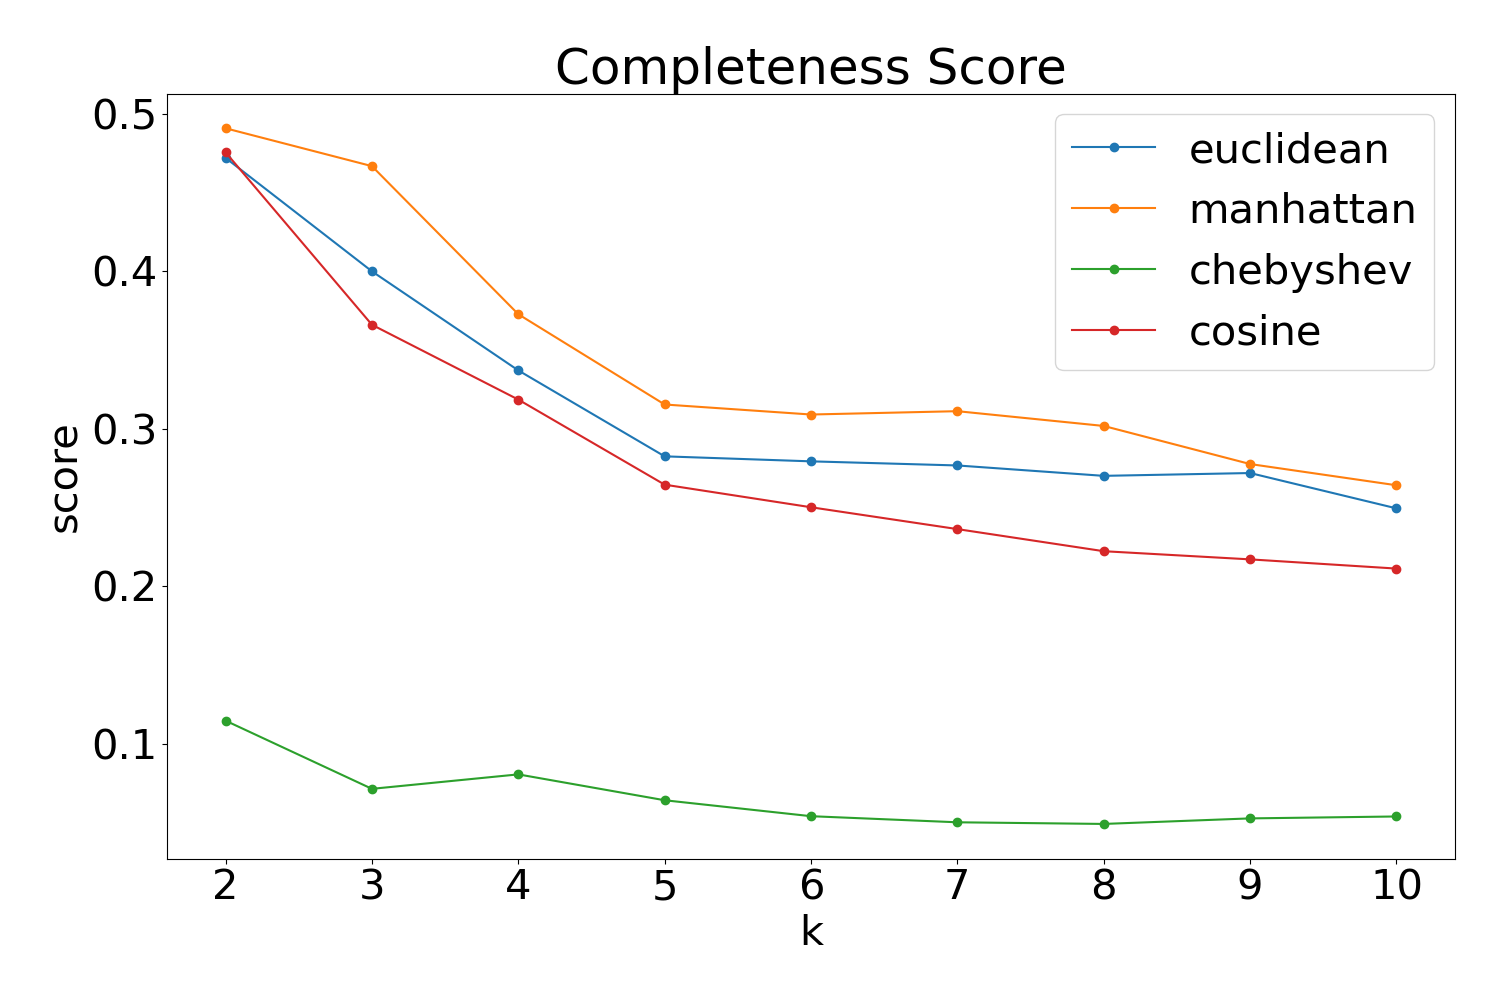
\includegraphics[width=0.45\textwidth]{../plots/housevotes/kmeans/Completeness Score/k_1to10.png} }}%
	\qquad
	\subfloat[Homogeneity Score ]{{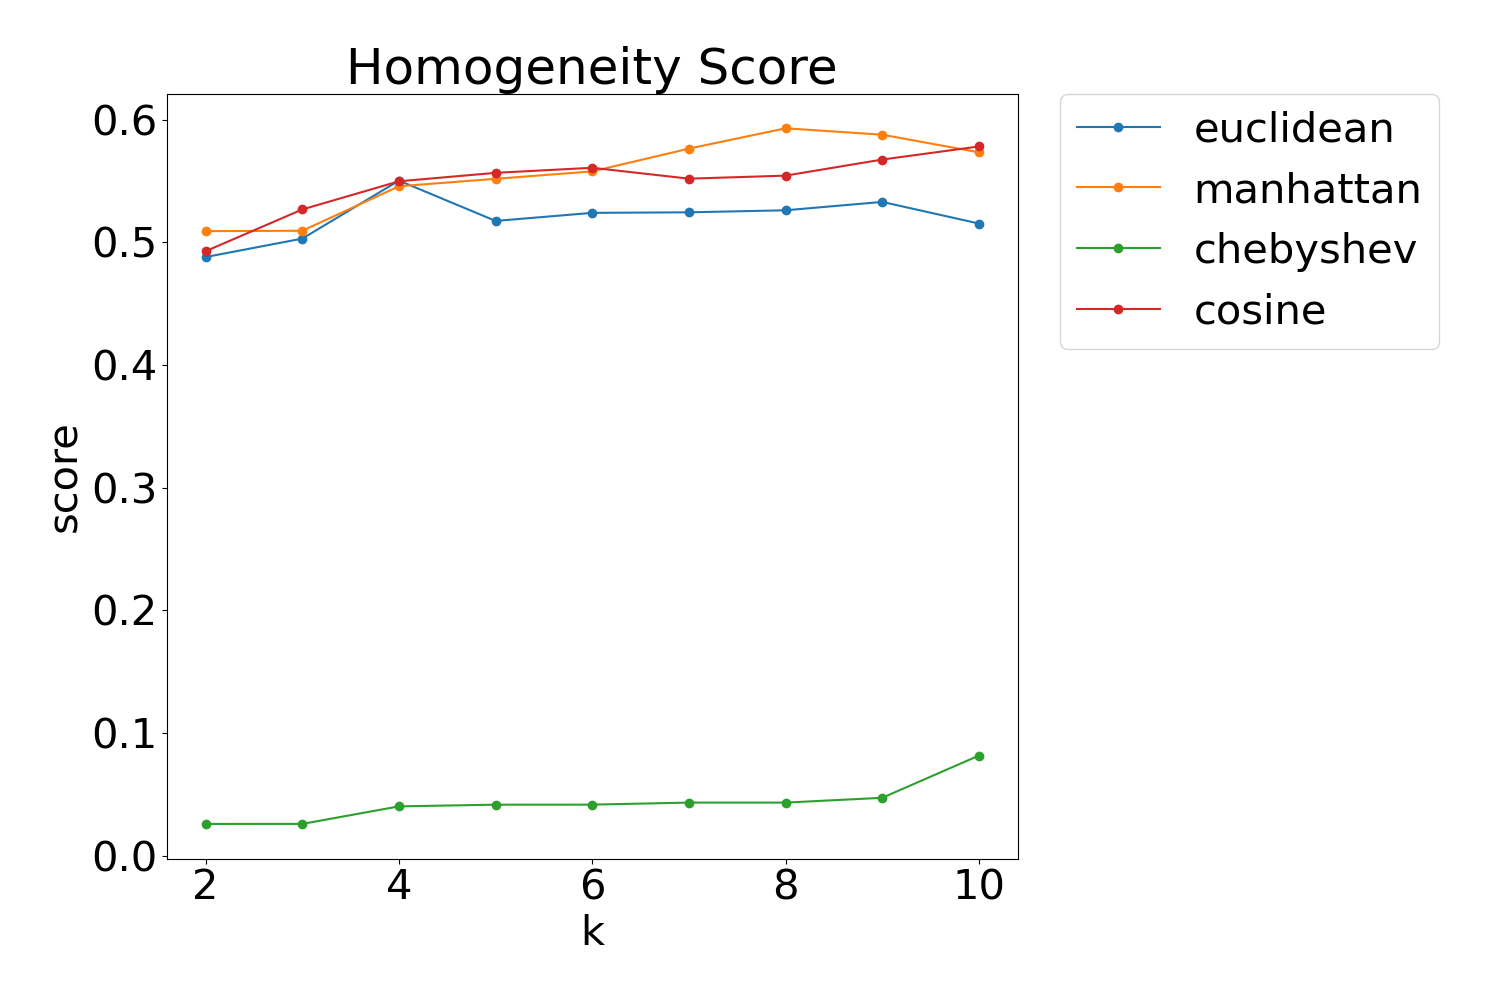
\includegraphics[width=0.45\textwidth]{../plots/housevotes/kmeans/Homogeneity Score/k_1to10.png} }}%
	\qquad
	\subfloat[Silhouette Score ]{{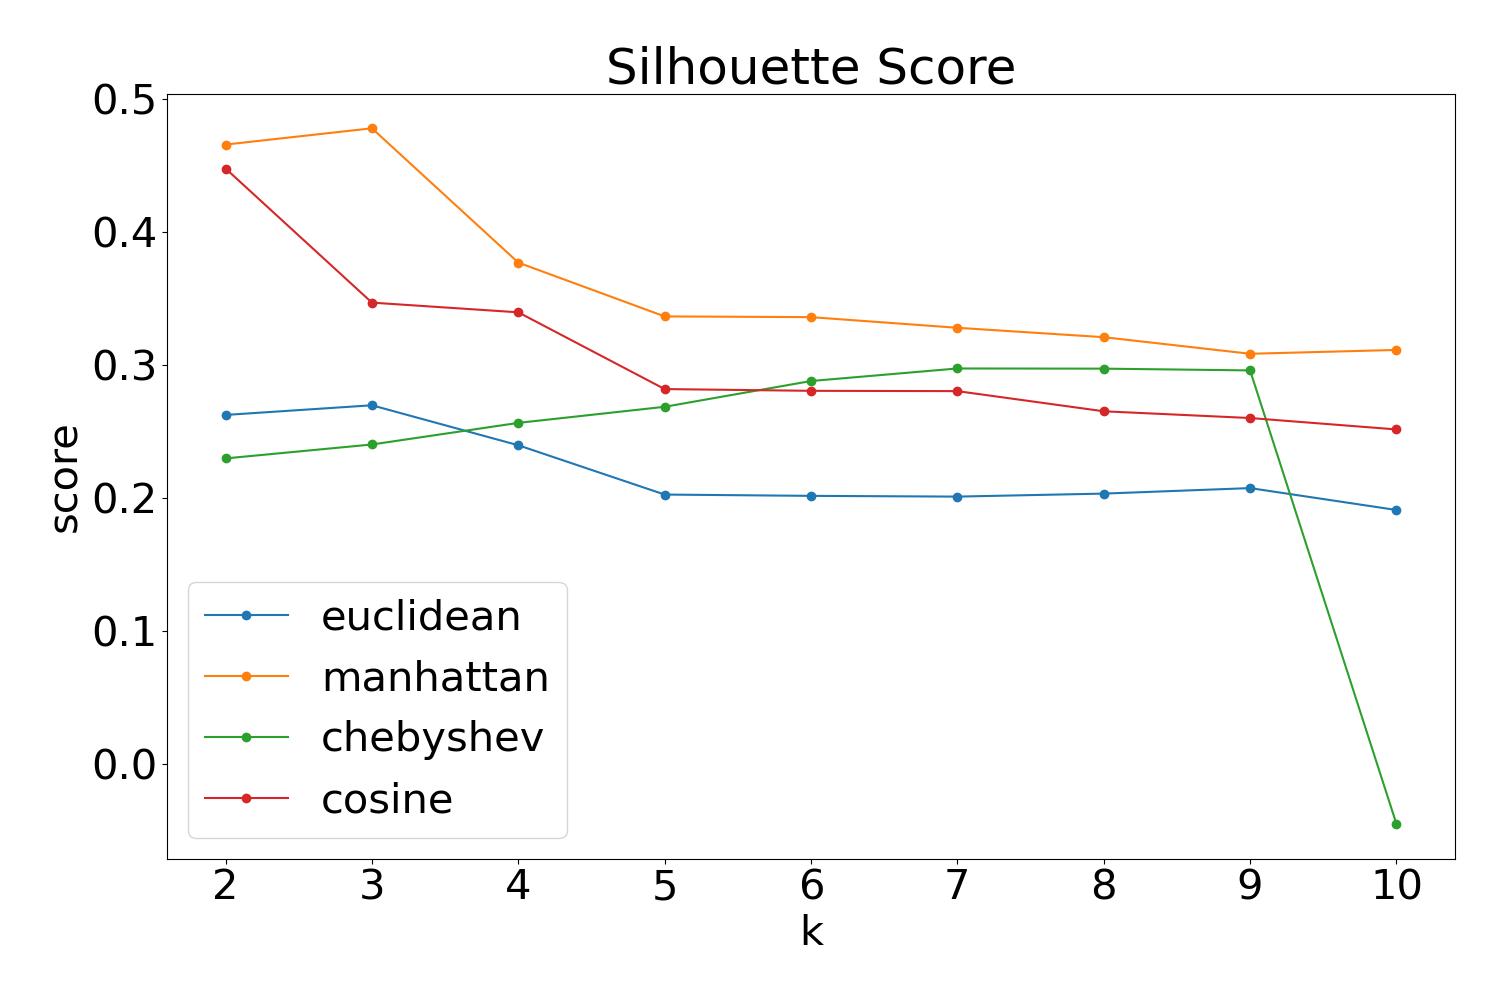
\includegraphics[width=1\textwidth]{../plots/housevotes/kmeans/Silhouette Score/k_1to10.png} }}%
	
	\caption{Comparison of clustering scores for kmeans-clustering on Housevotes dataset}%
\end{figure}

\begin{figure}[H]
	\centering
	\subfloat[ARI ]{{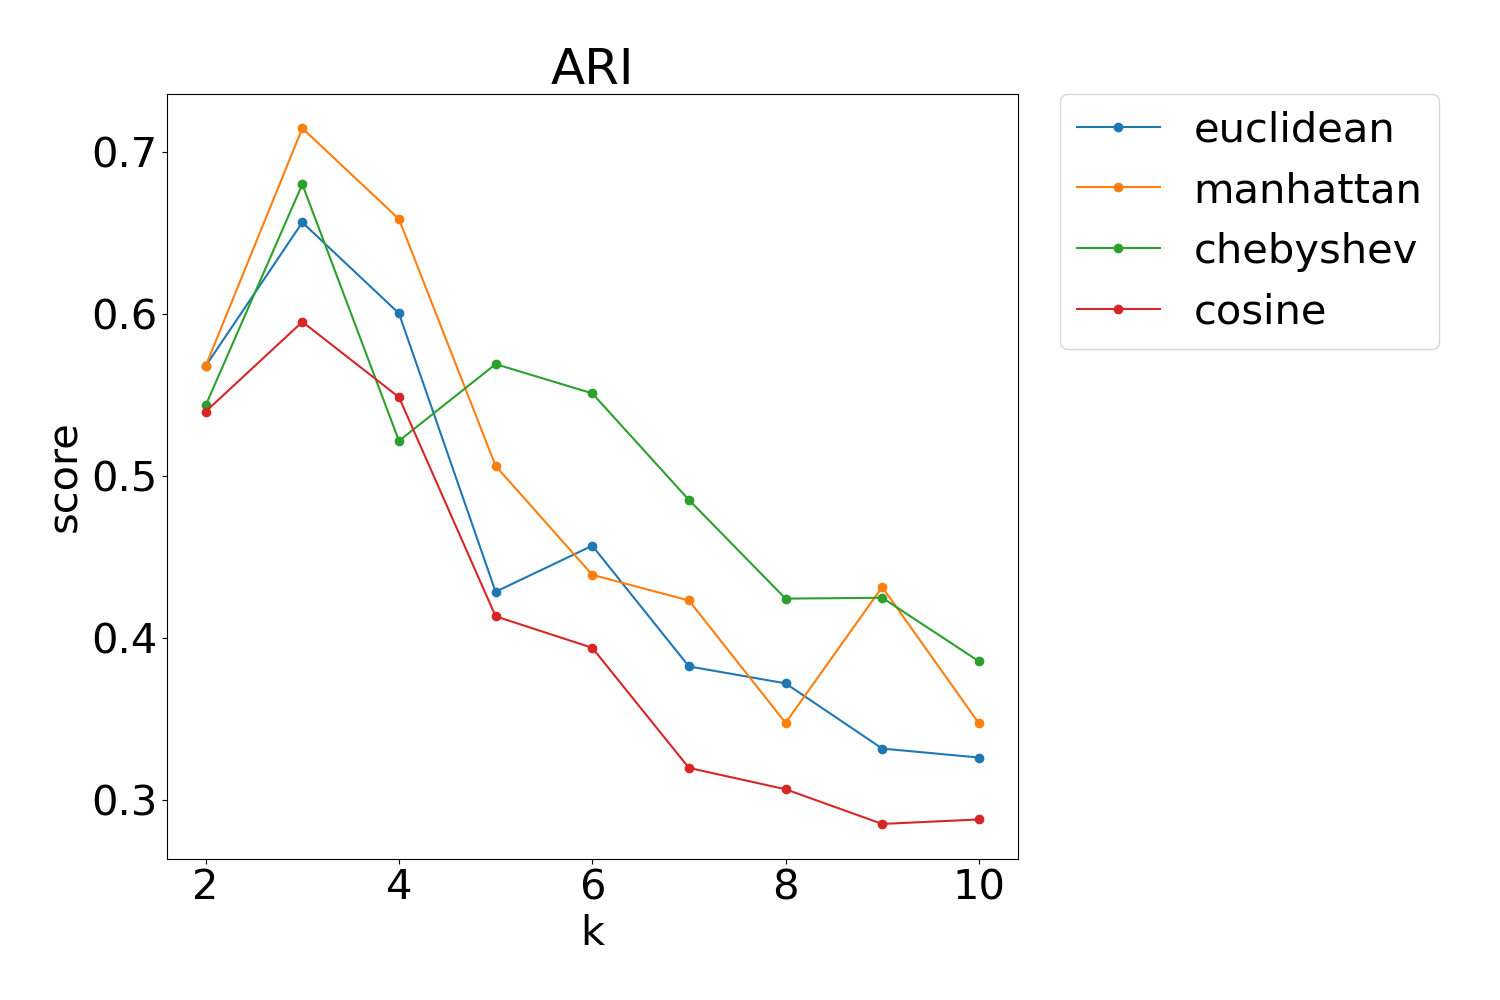
\includegraphics[width=0.45\textwidth]{../plots/iris/kmedians/ARI/k_1to10.png} }}%
	\qquad
	\subfloat[NMI ]{{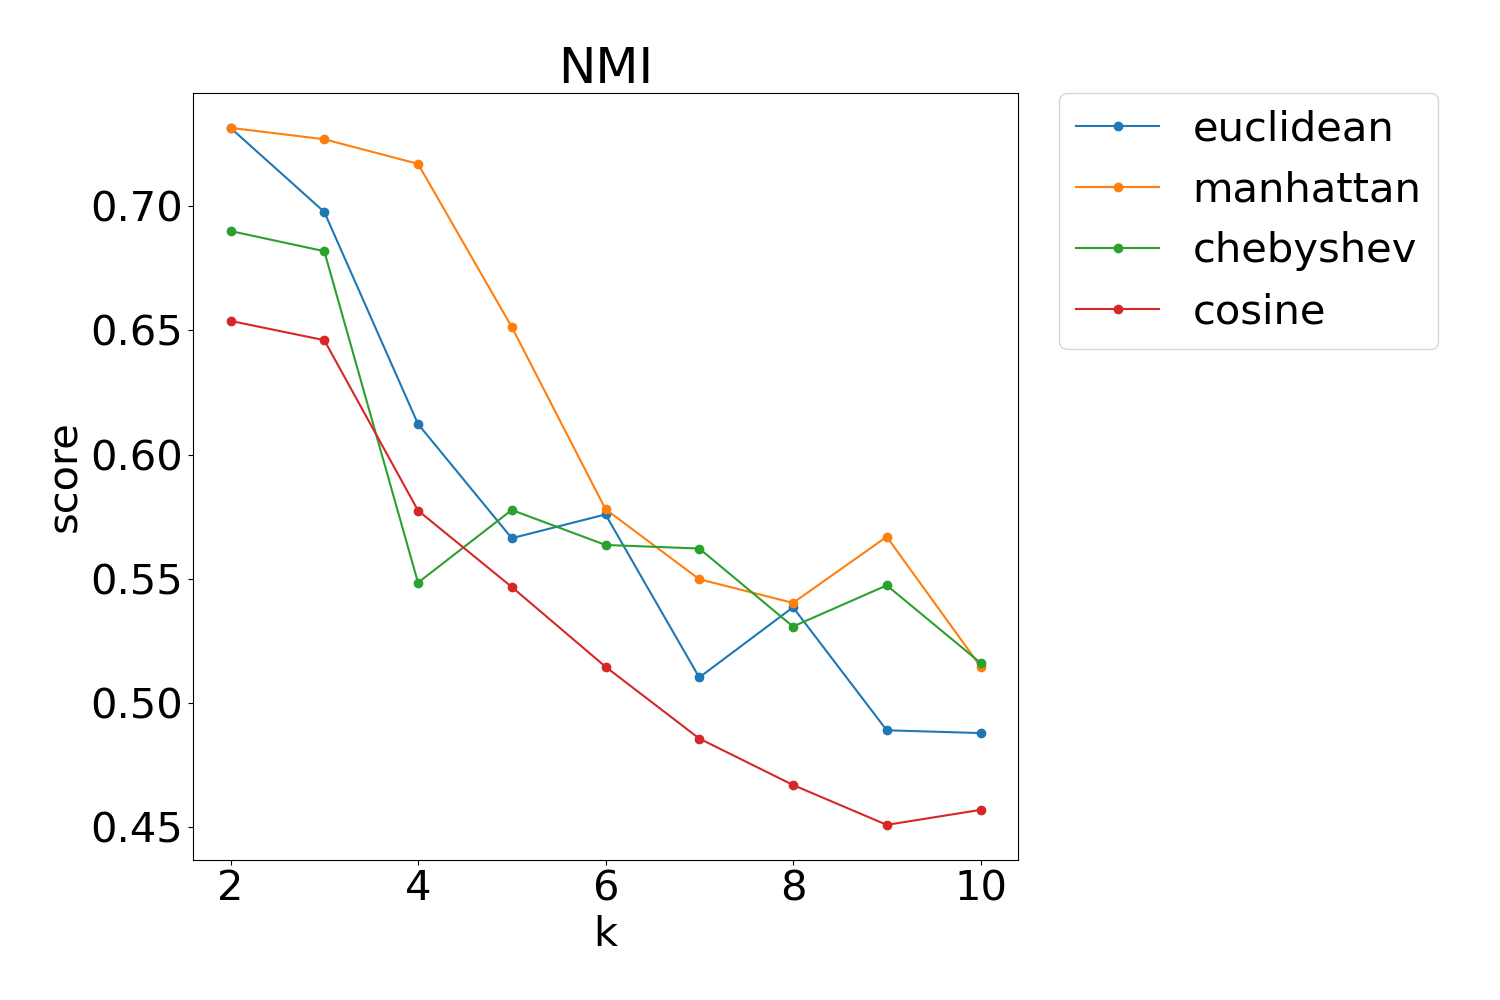
\includegraphics[width=0.45\textwidth]{../plots/iris/kmedians/NMI/k_1to10.png} }}%
	\qquad
	\subfloat[Completeness Score ]{{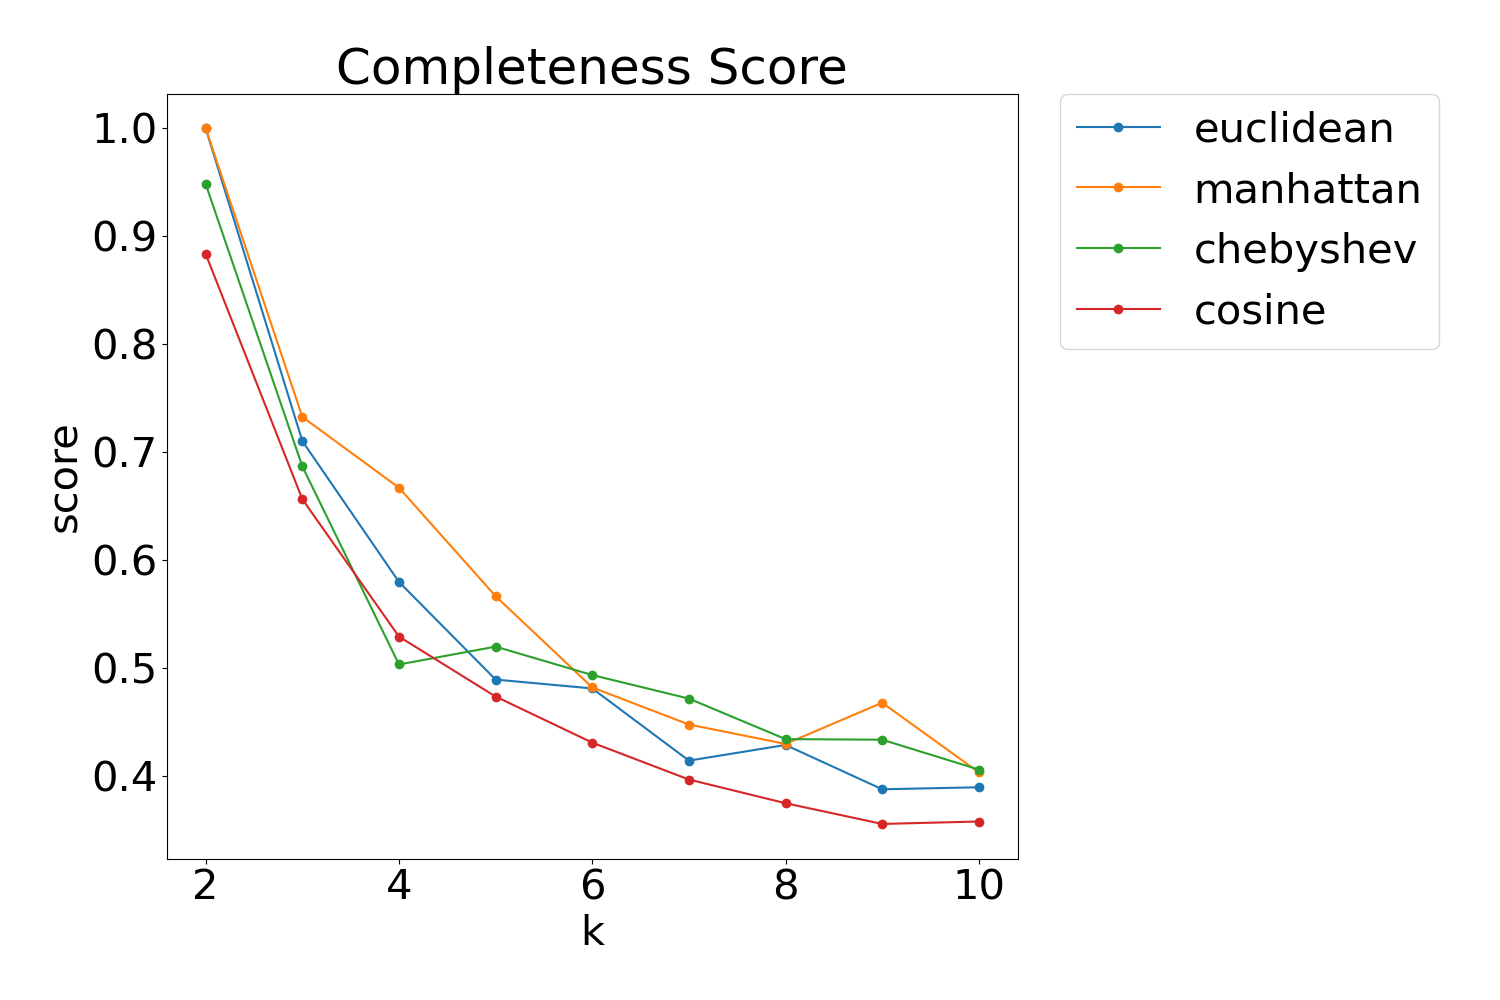
\includegraphics[width=0.45\textwidth]{../plots/iris/kmedians/Completeness Score/k_1to10.png} }}%
	\qquad
	\subfloat[Homogeneity Score ]{{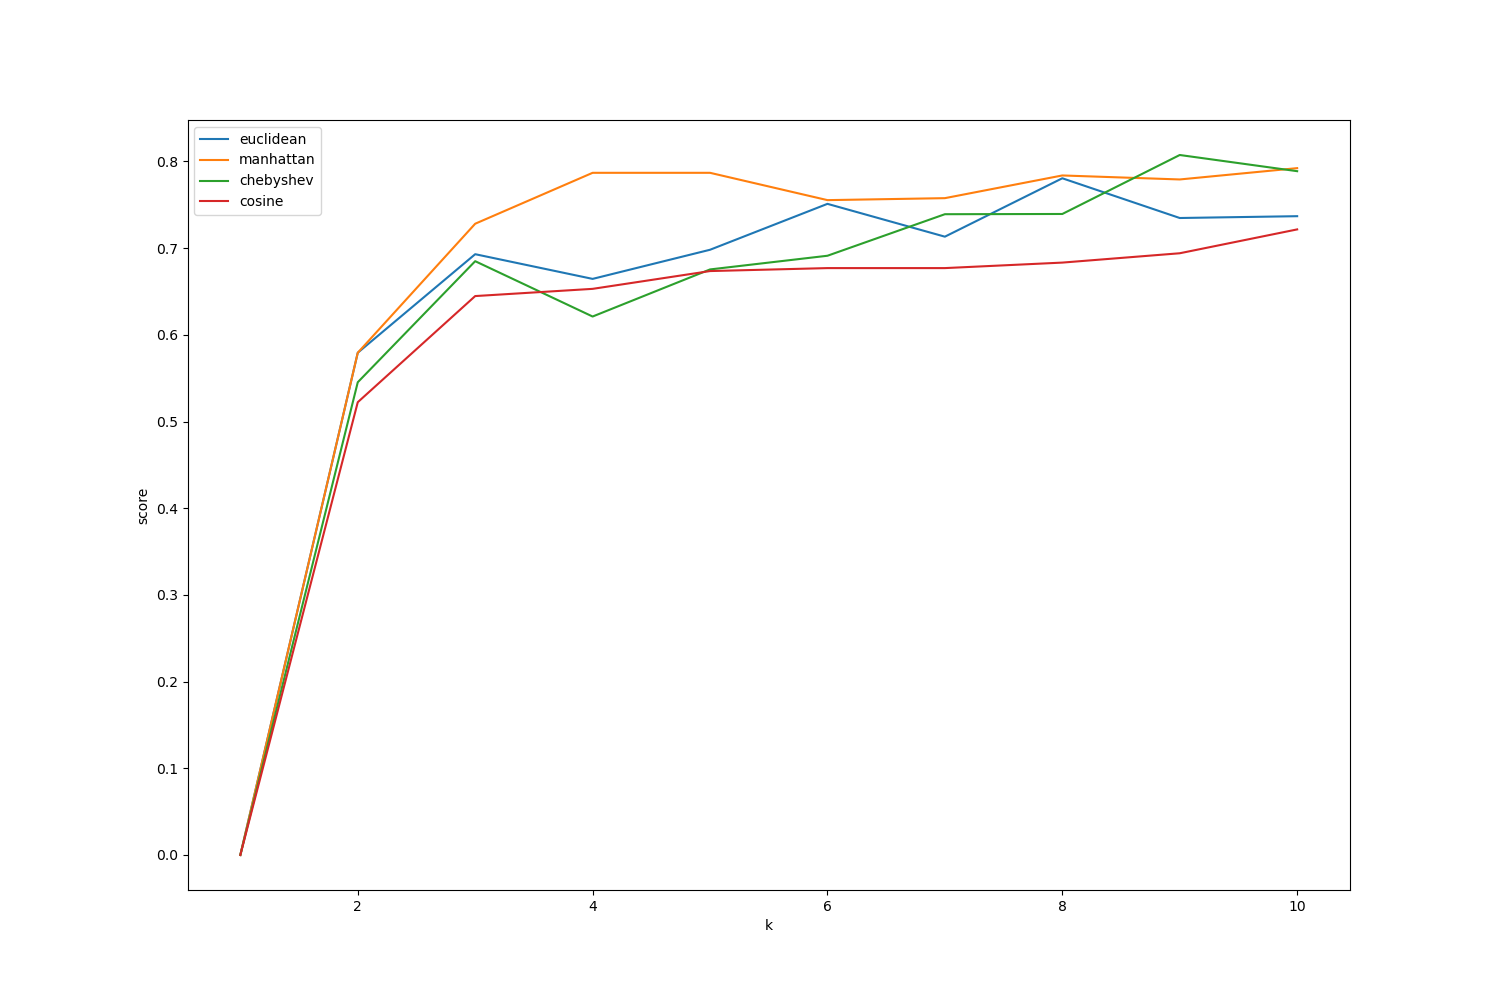
\includegraphics[width=0.45\textwidth]{../plots/iris/kmedians/Homogeneity Score/k_1to10.png} }}%
	\qquad
	\subfloat[Silhouette Score ]{{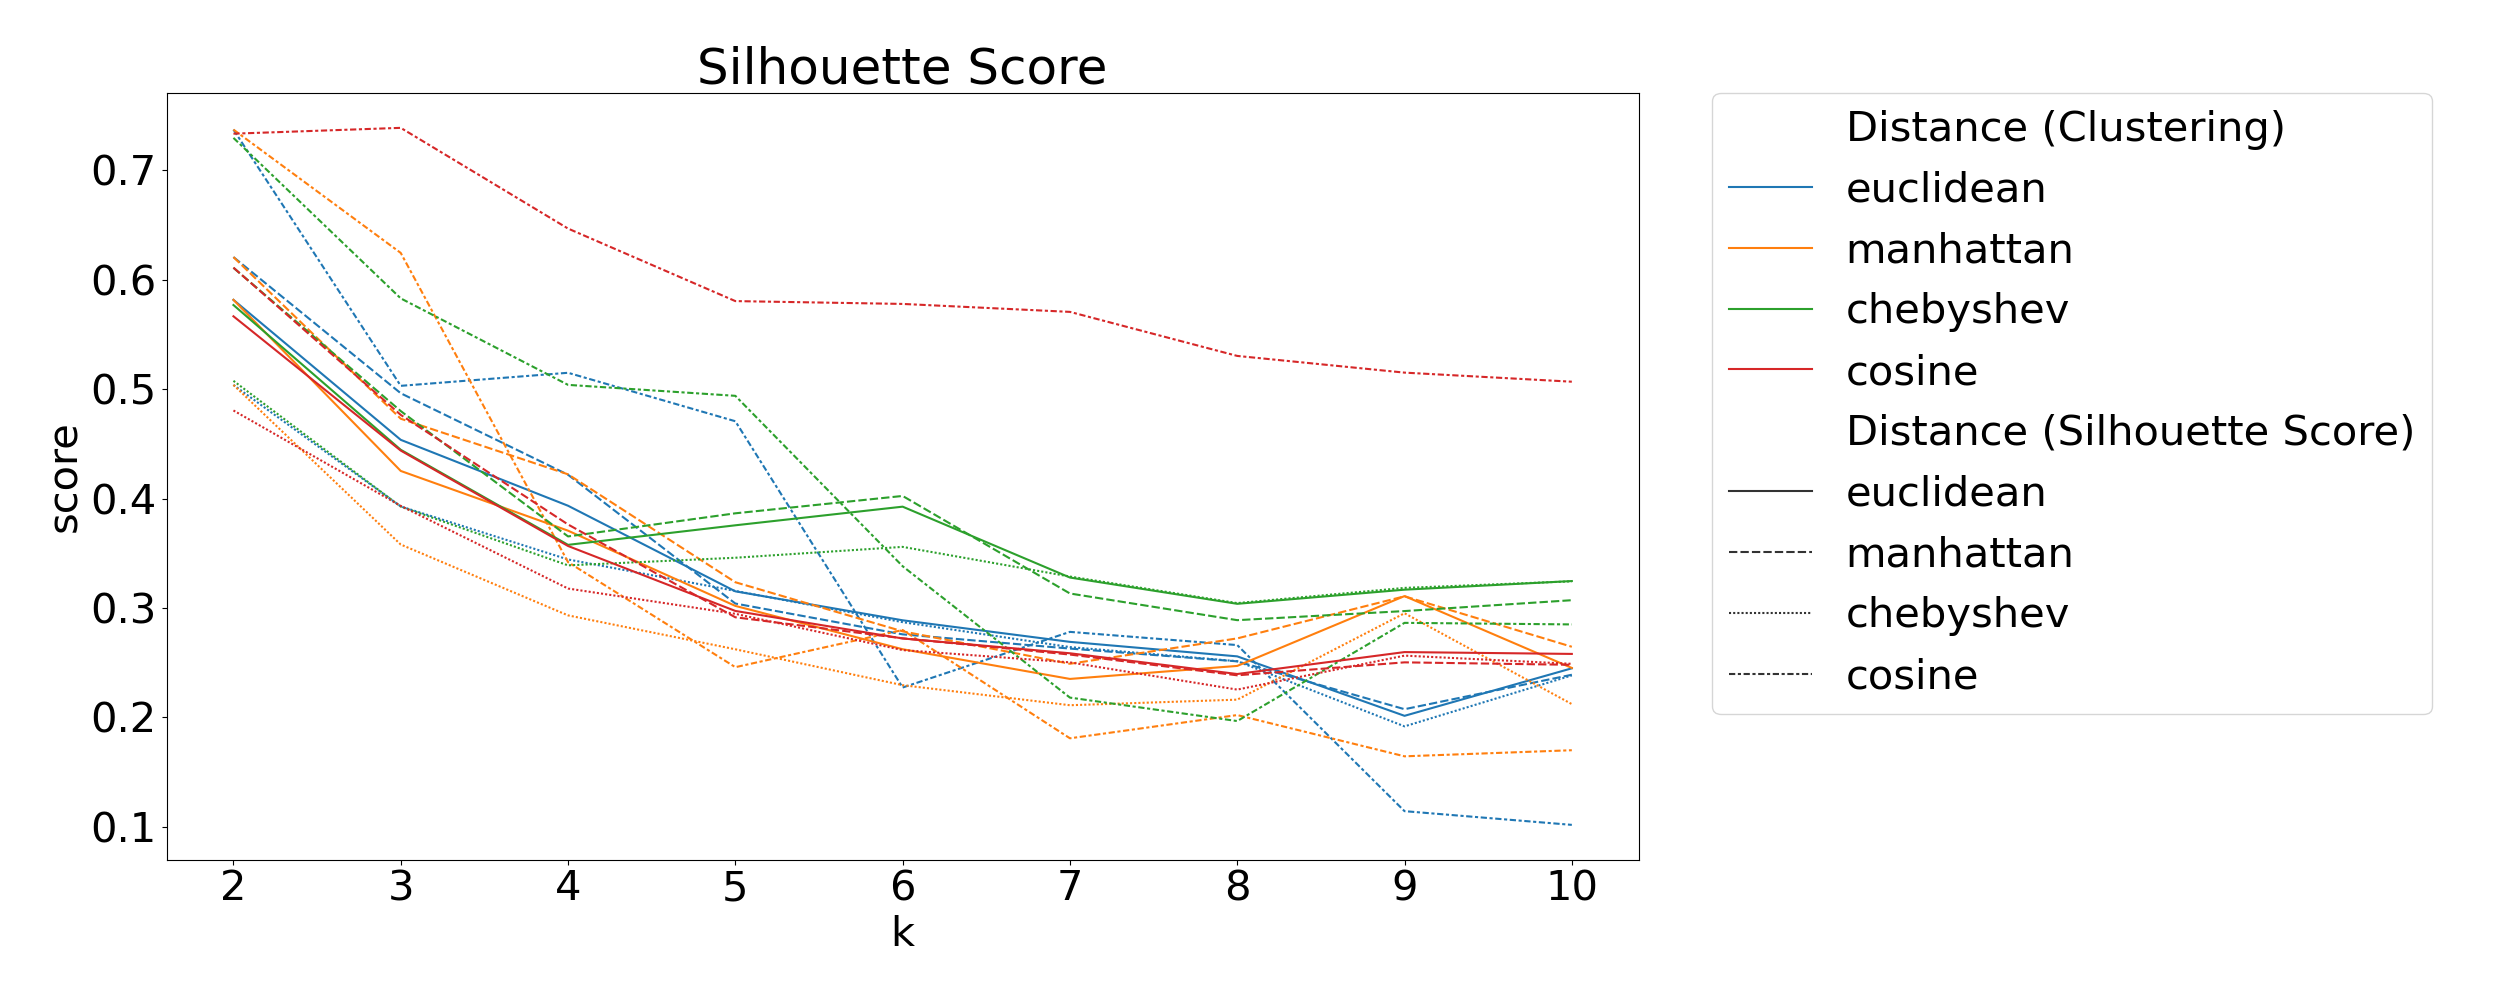
\includegraphics[width=1\textwidth]{../plots/iris/kmedians/Silhouette Score/k_1to10.png} }}%
	
	\caption{Comparison of clustering scores for kmedians-clustering on Iris dataset}%
\end{figure}

\begin{figure}[H]
	\centering
	\subfloat[ARI ]{{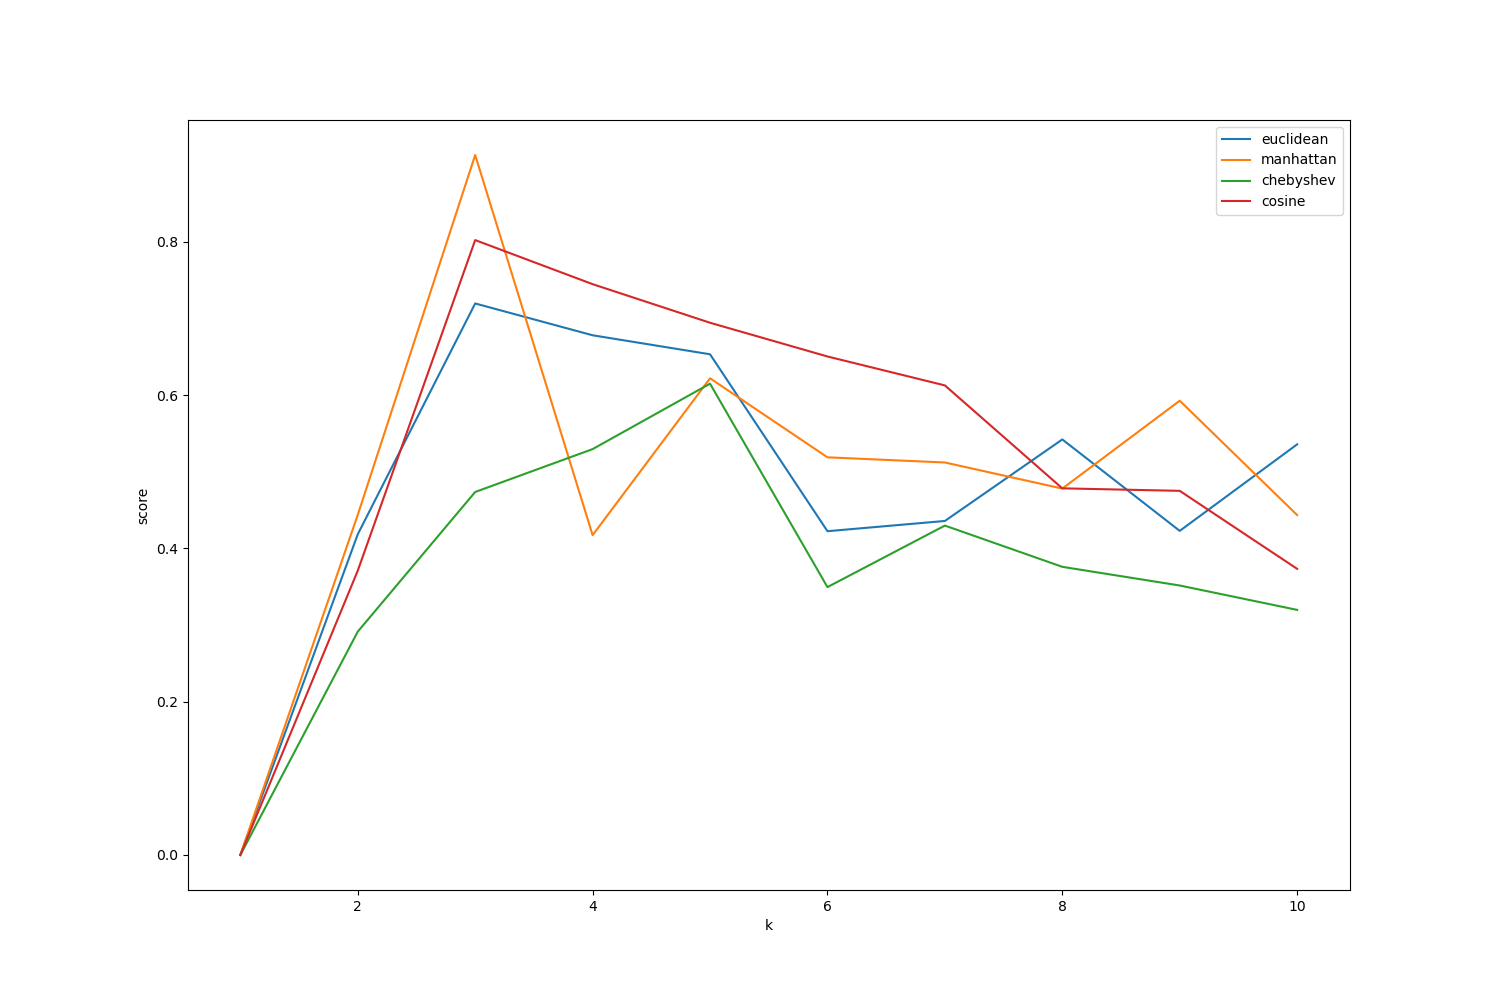
\includegraphics[width=0.45\textwidth]{../plots/wine/kmedians/ARI/k_1to10.png} }}%
	\qquad
	\subfloat[NMI ]{{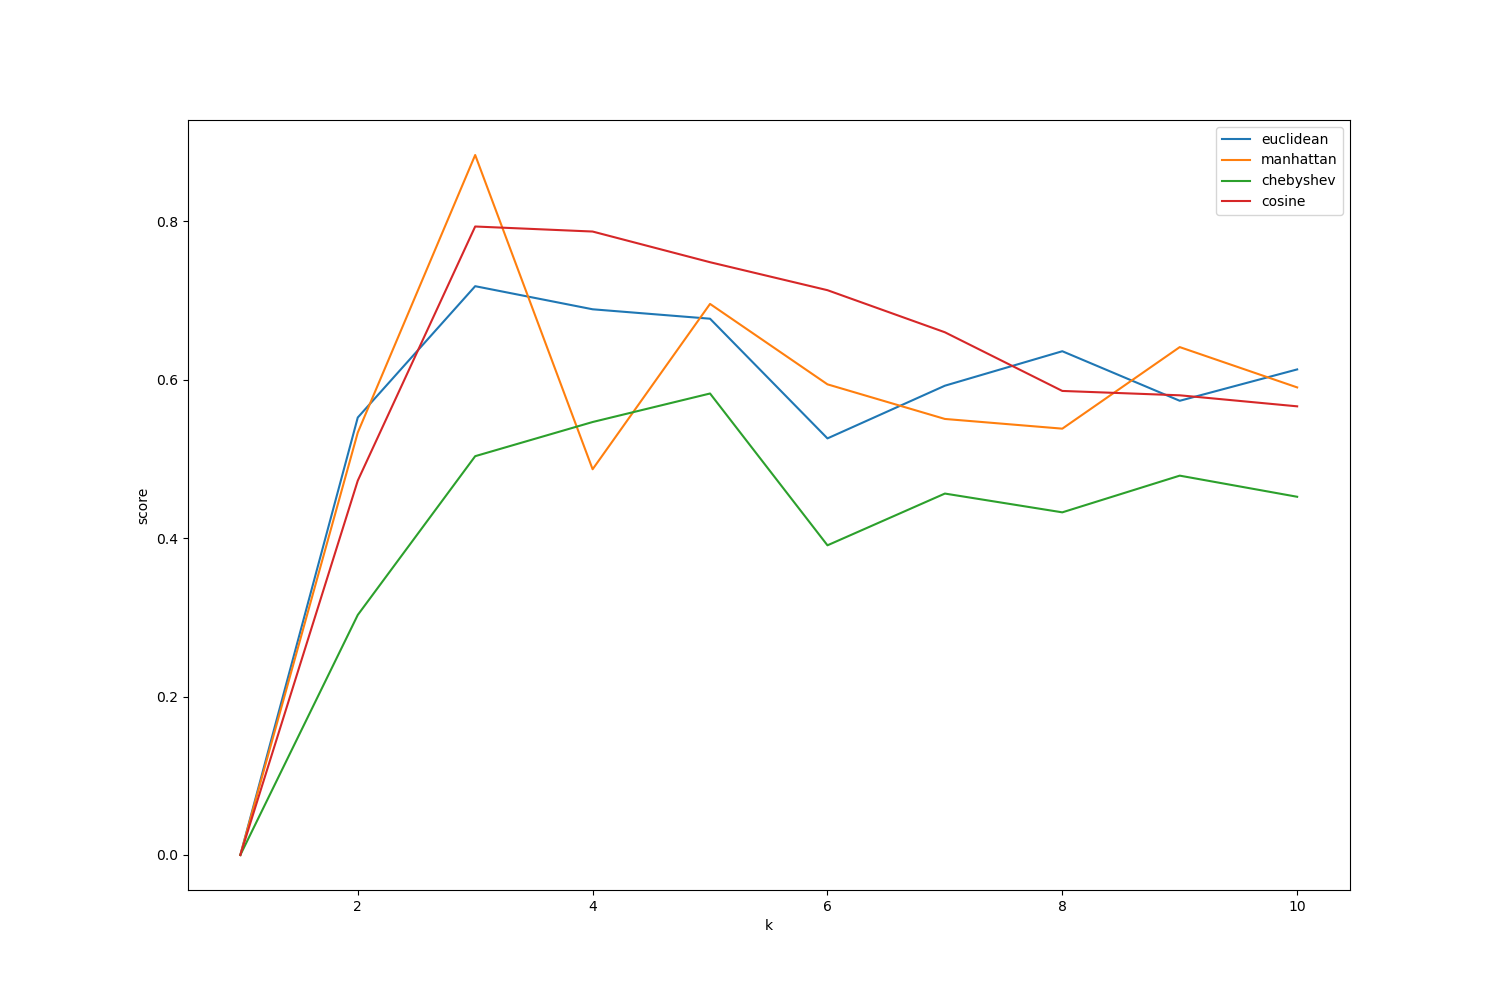
\includegraphics[width=0.45\textwidth]{../plots/wine/kmedians/NMI/k_1to10.png} }}%
	\qquad
	\subfloat[Completeness Score ]{{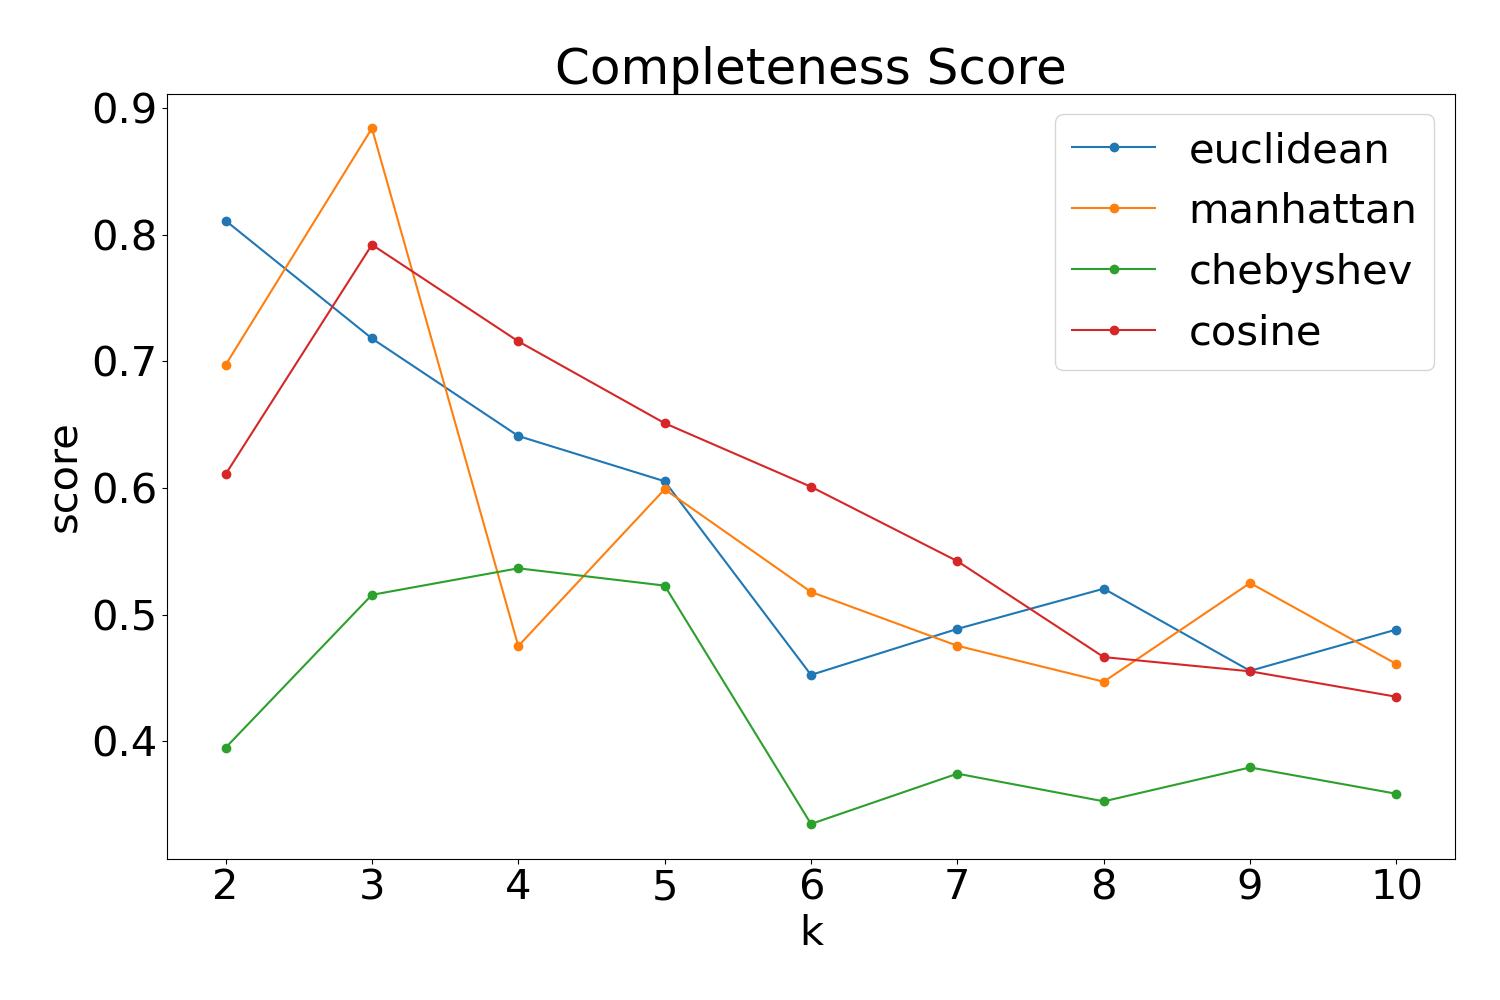
\includegraphics[width=0.45\textwidth]{../plots/wine/kmedians/Completeness Score/k_1to10.png} }}%
	\qquad
	\subfloat[Homogeneity Score ]{{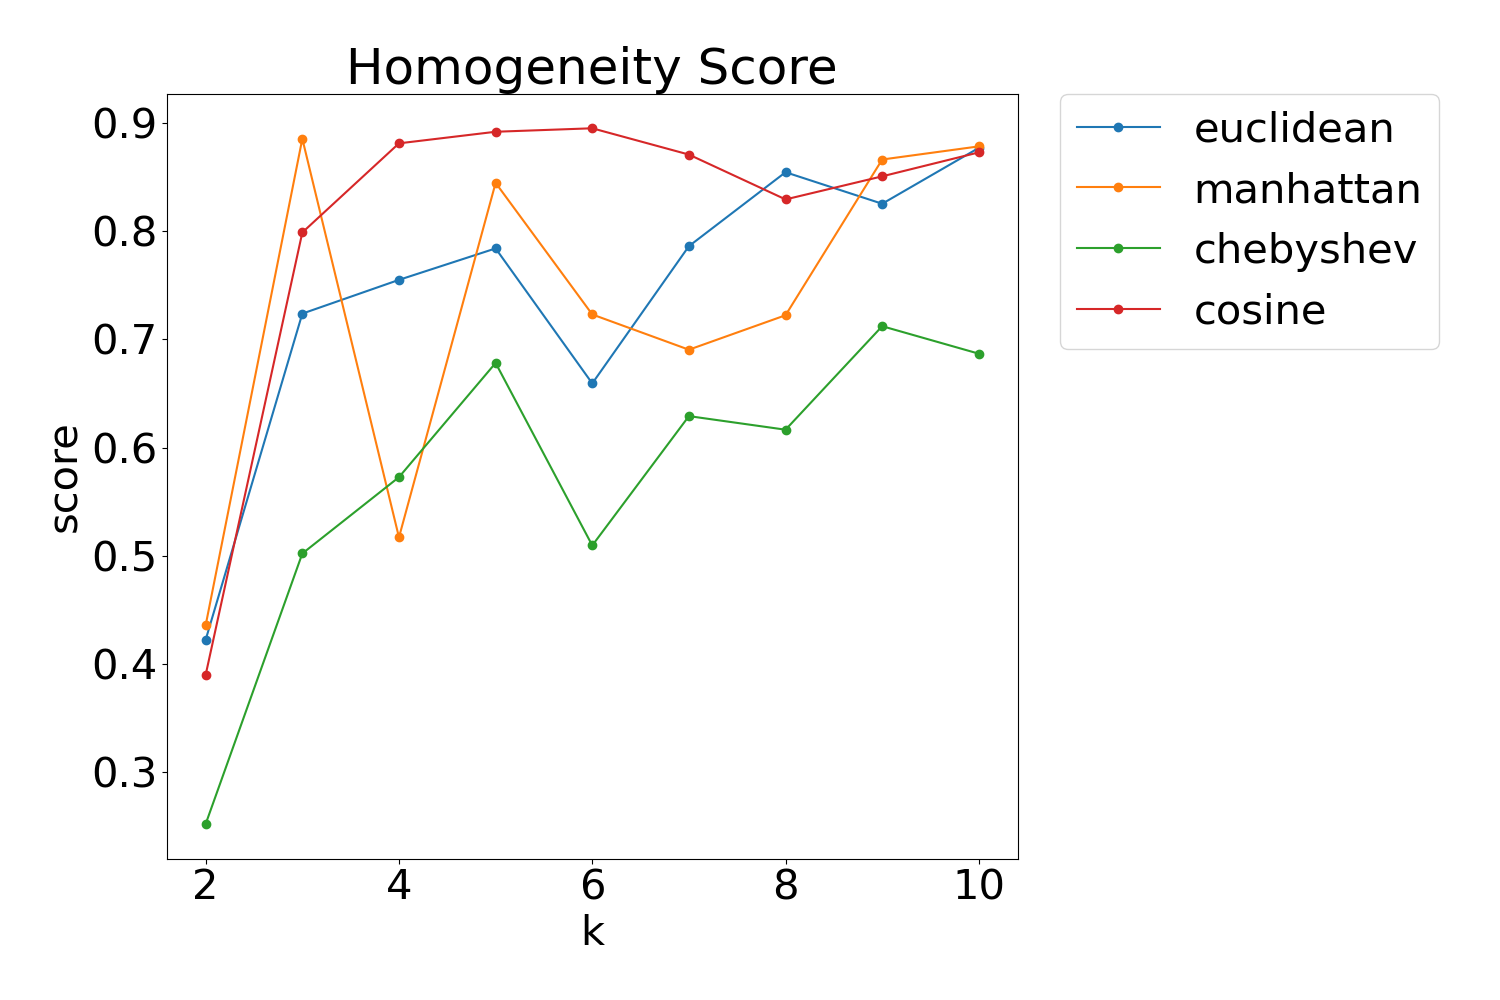
\includegraphics[width=0.45\textwidth]{../plots/wine/kmedians/Homogeneity Score/k_1to10.png} }}%
	\qquad
	\subfloat[Silhouette Score ]{{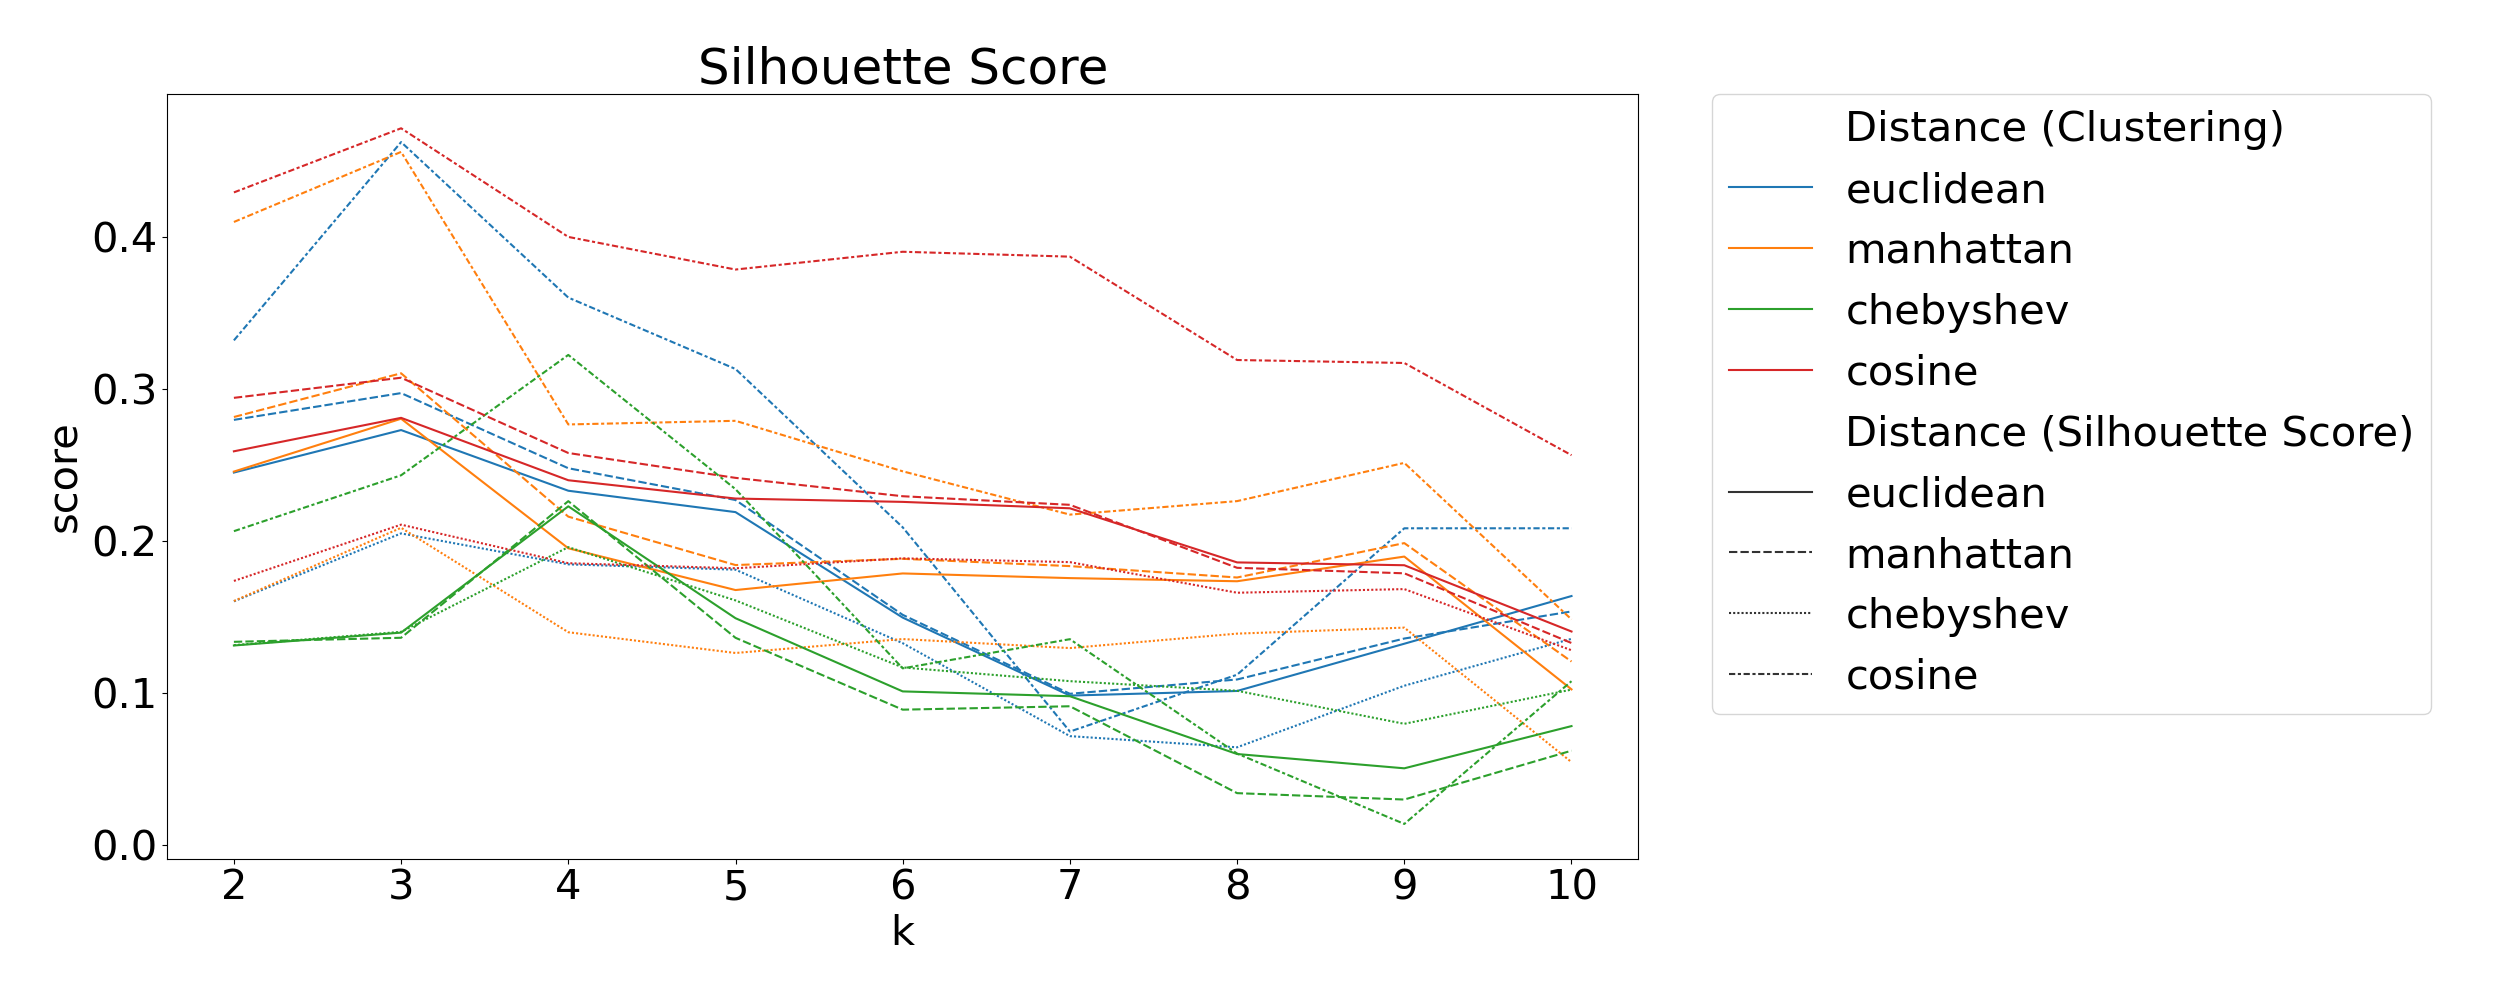
\includegraphics[width=1\textwidth]{../plots/wine/kmedians/Silhouette Score/k_1to10.png} }}%
	
	\caption{Comparison of clustering scores for kmedians-clustering on Wine dataset}%
\end{figure}

\begin{figure}[H]
	\centering
	\subfloat[Silhouette Score ]{{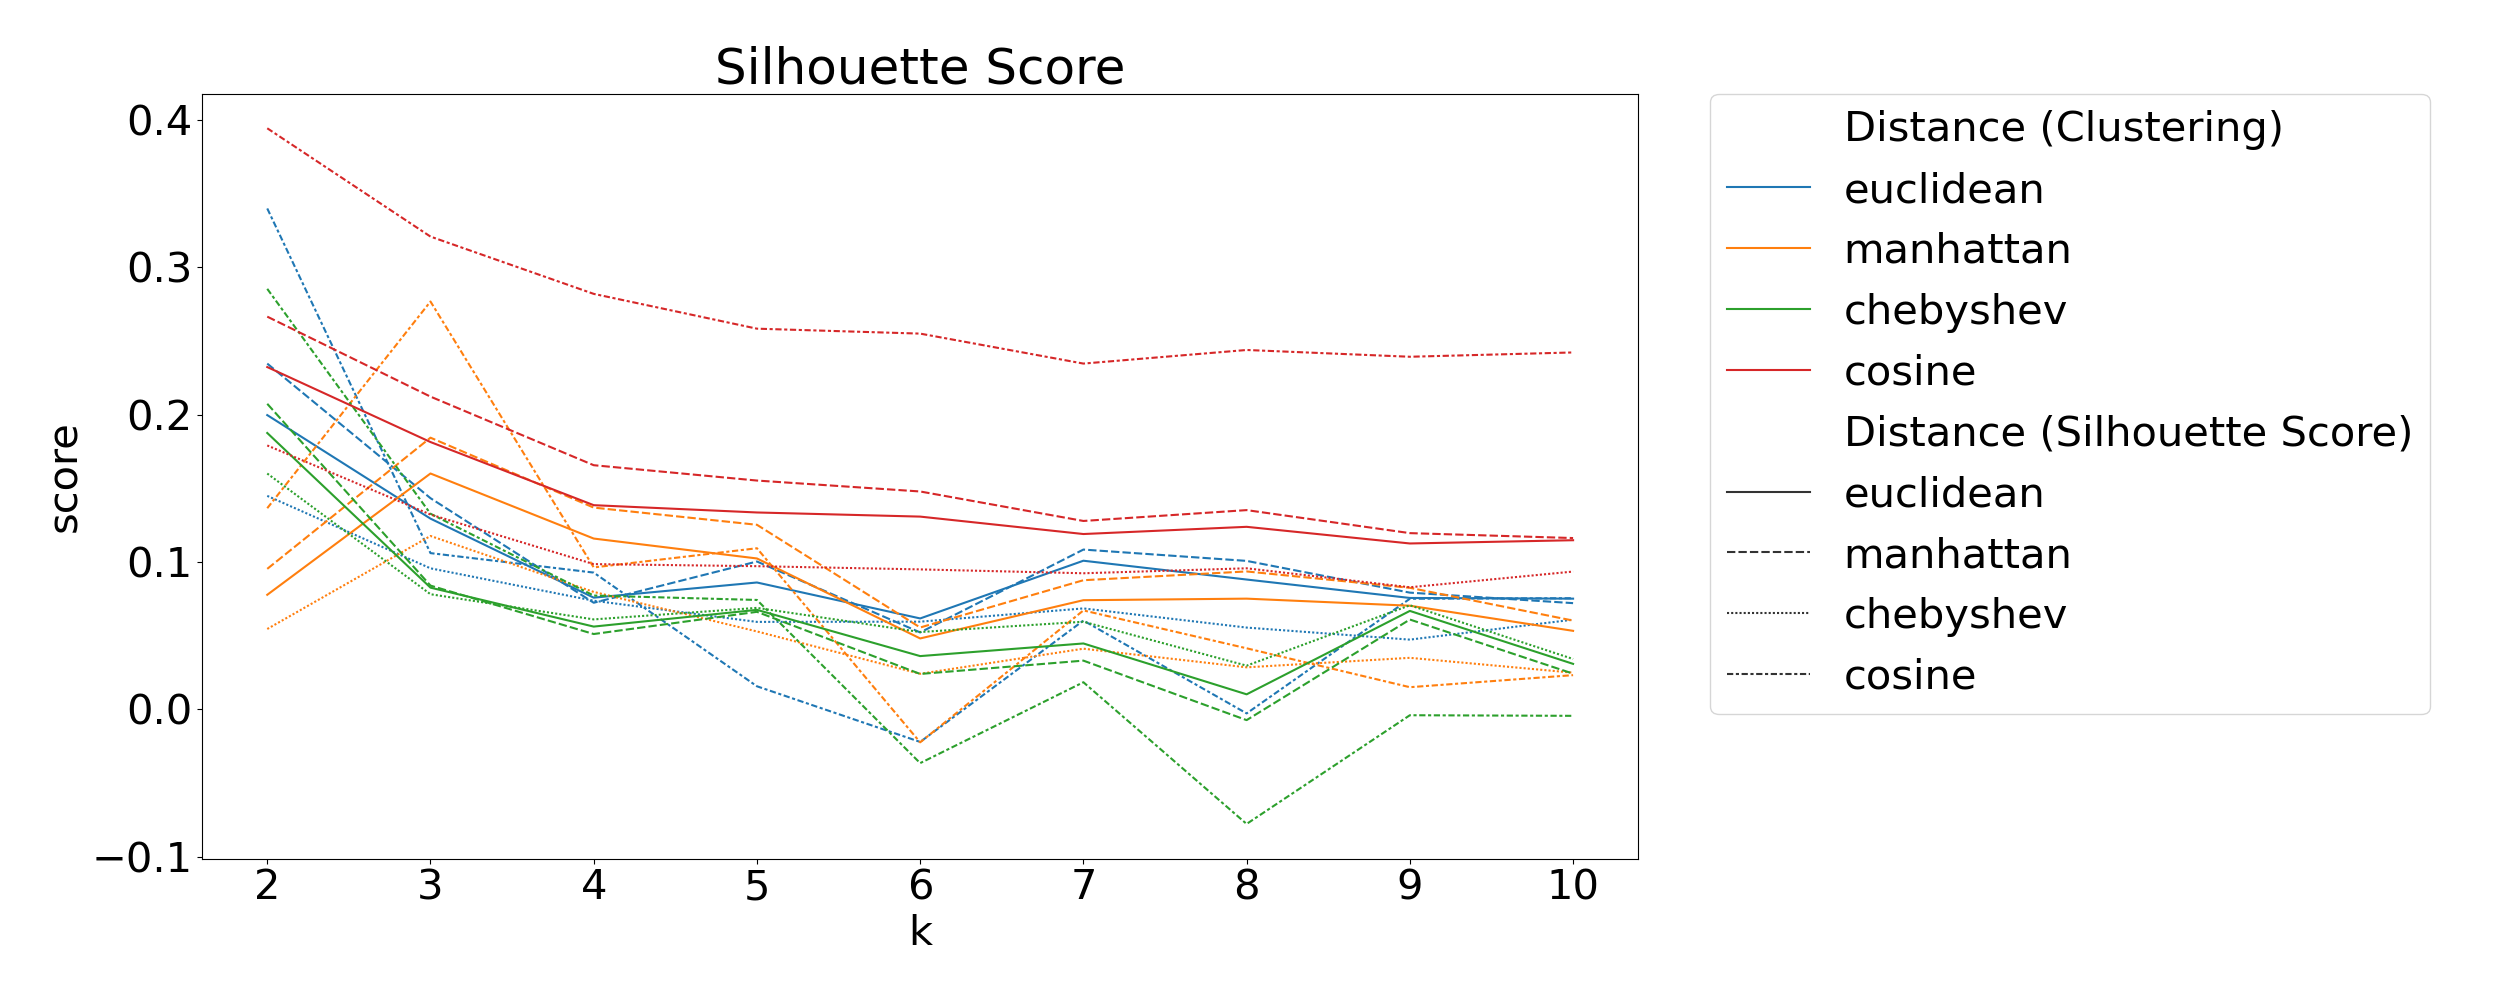
\includegraphics[width=1\textwidth]{../plots/diabetes/kmedians/Silhouette Score/k_1to10.png} }}%
	
	\caption{Comparison of clustering scores for kmedians-clustering on Diabetes dataset}%
\end{figure}

\begin{figure}[H]
	\centering
	\subfloat[ARI ]{{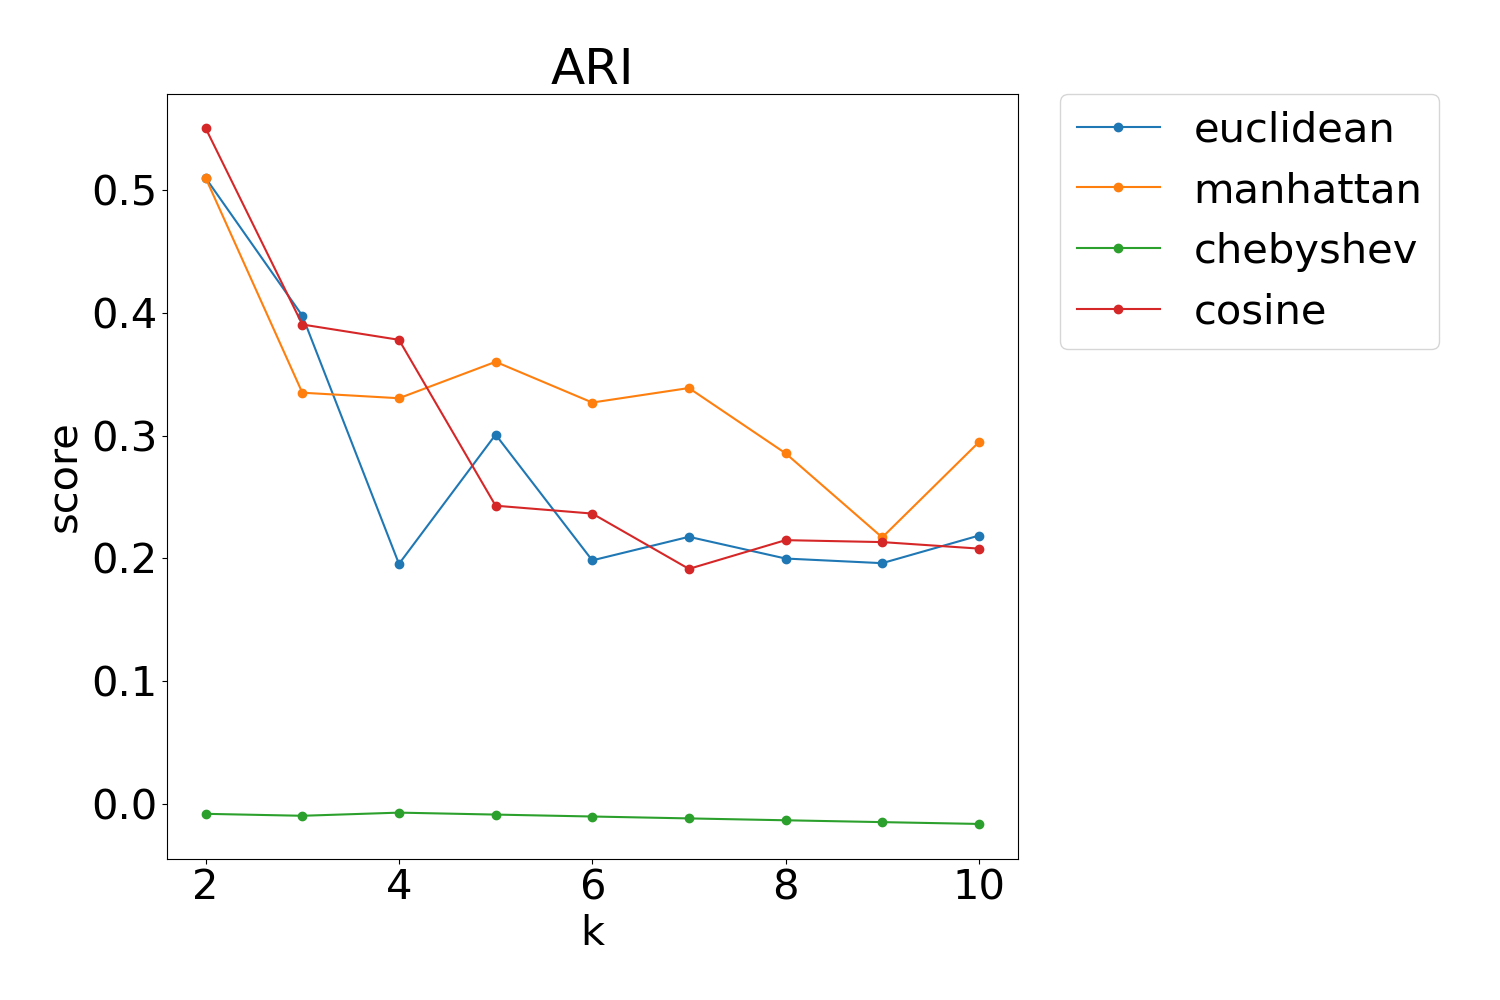
\includegraphics[width=0.45\textwidth]{../plots/housevotes/kmedians/ARI/k_1to10.png} }}%
	\qquad
	\subfloat[NMI ]{{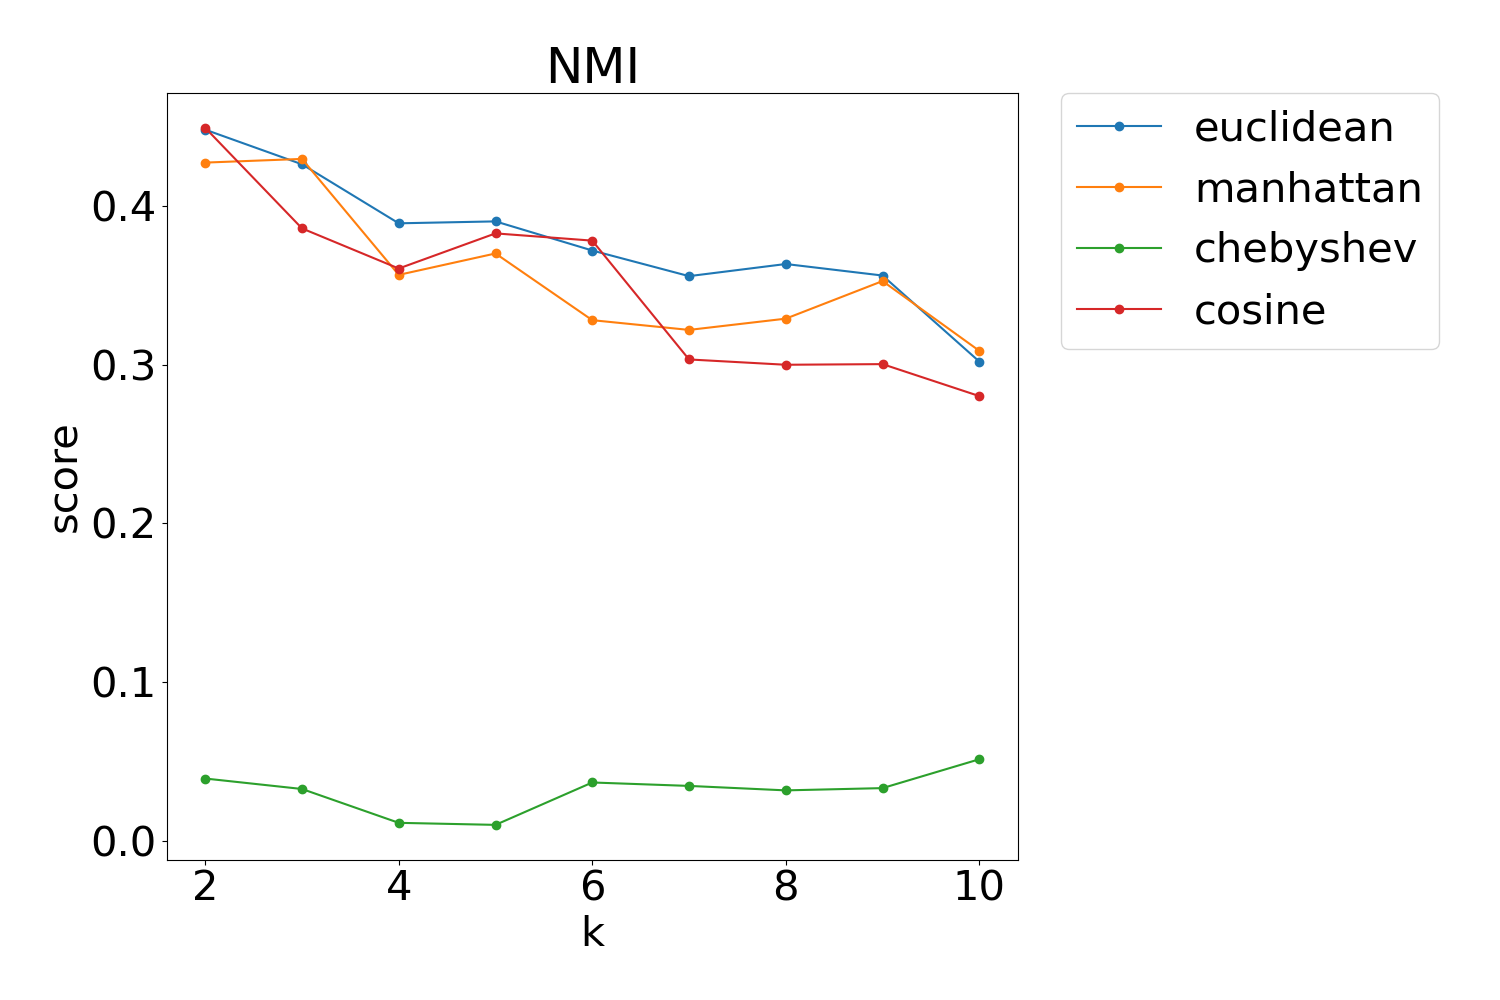
\includegraphics[width=0.45\textwidth]{../plots/housevotes/kmedians/NMI/k_1to10.png} }}%
	\qquad
	\subfloat[Completeness Score ]{{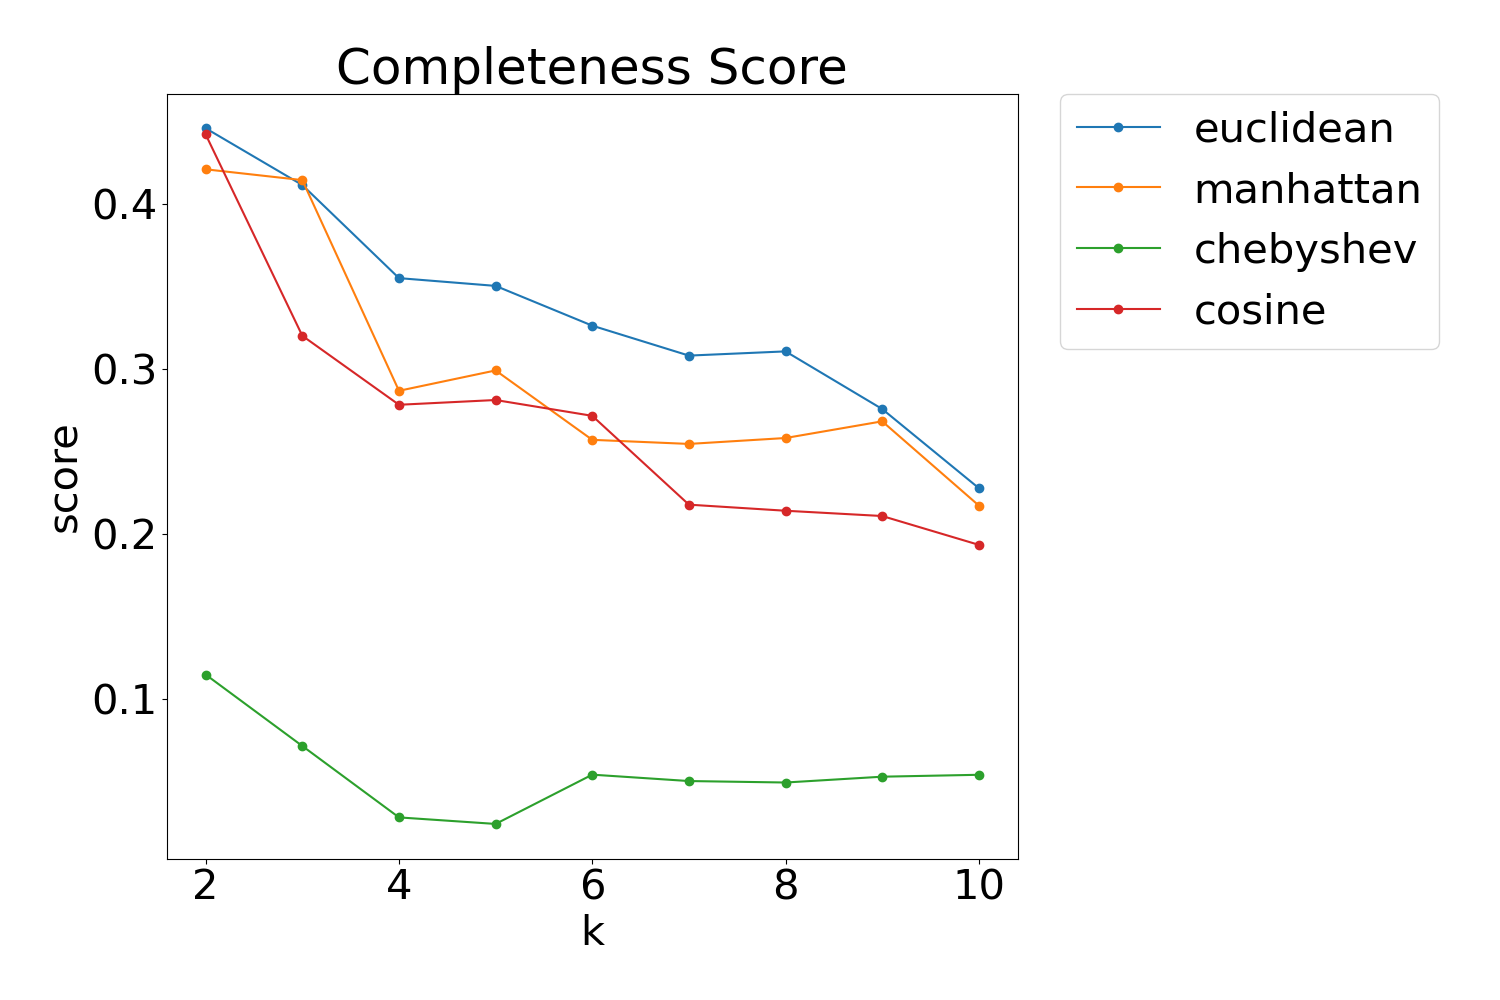
\includegraphics[width=0.45\textwidth]{../plots/housevotes/kmedians/Completeness Score/k_1to10.png} }}%
	\qquad
	\subfloat[Homogeneity Score ]{{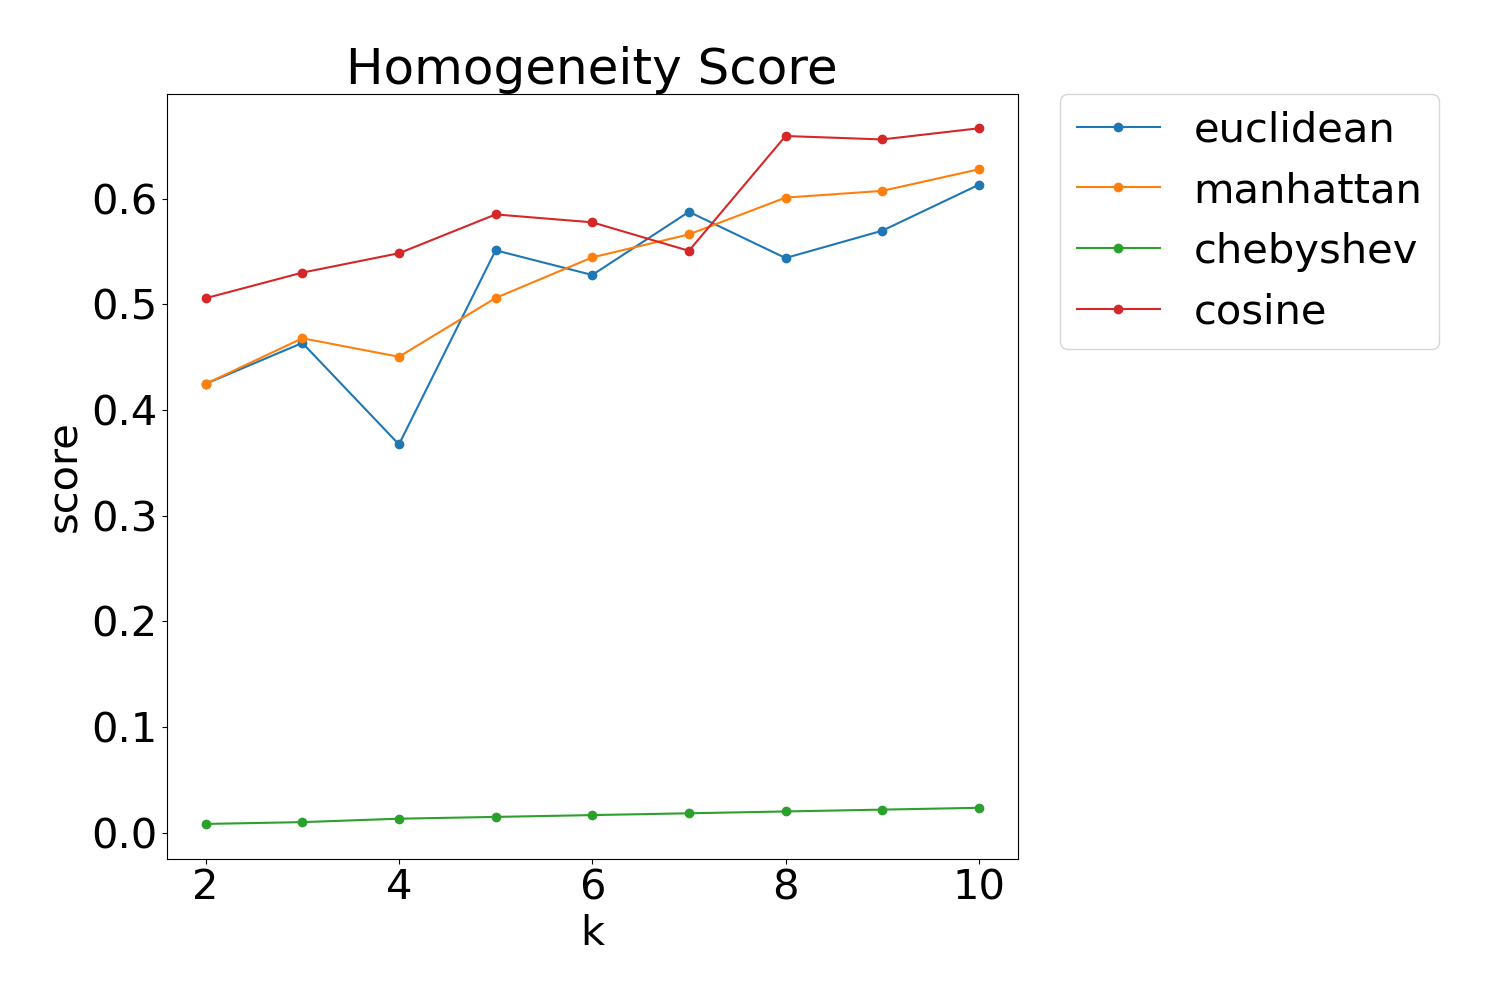
\includegraphics[width=0.45\textwidth]{../plots/housevotes/kmedians/Homogeneity Score/k_1to10.png} }}%
	\qquad
	\subfloat[Silhouette Score ]{{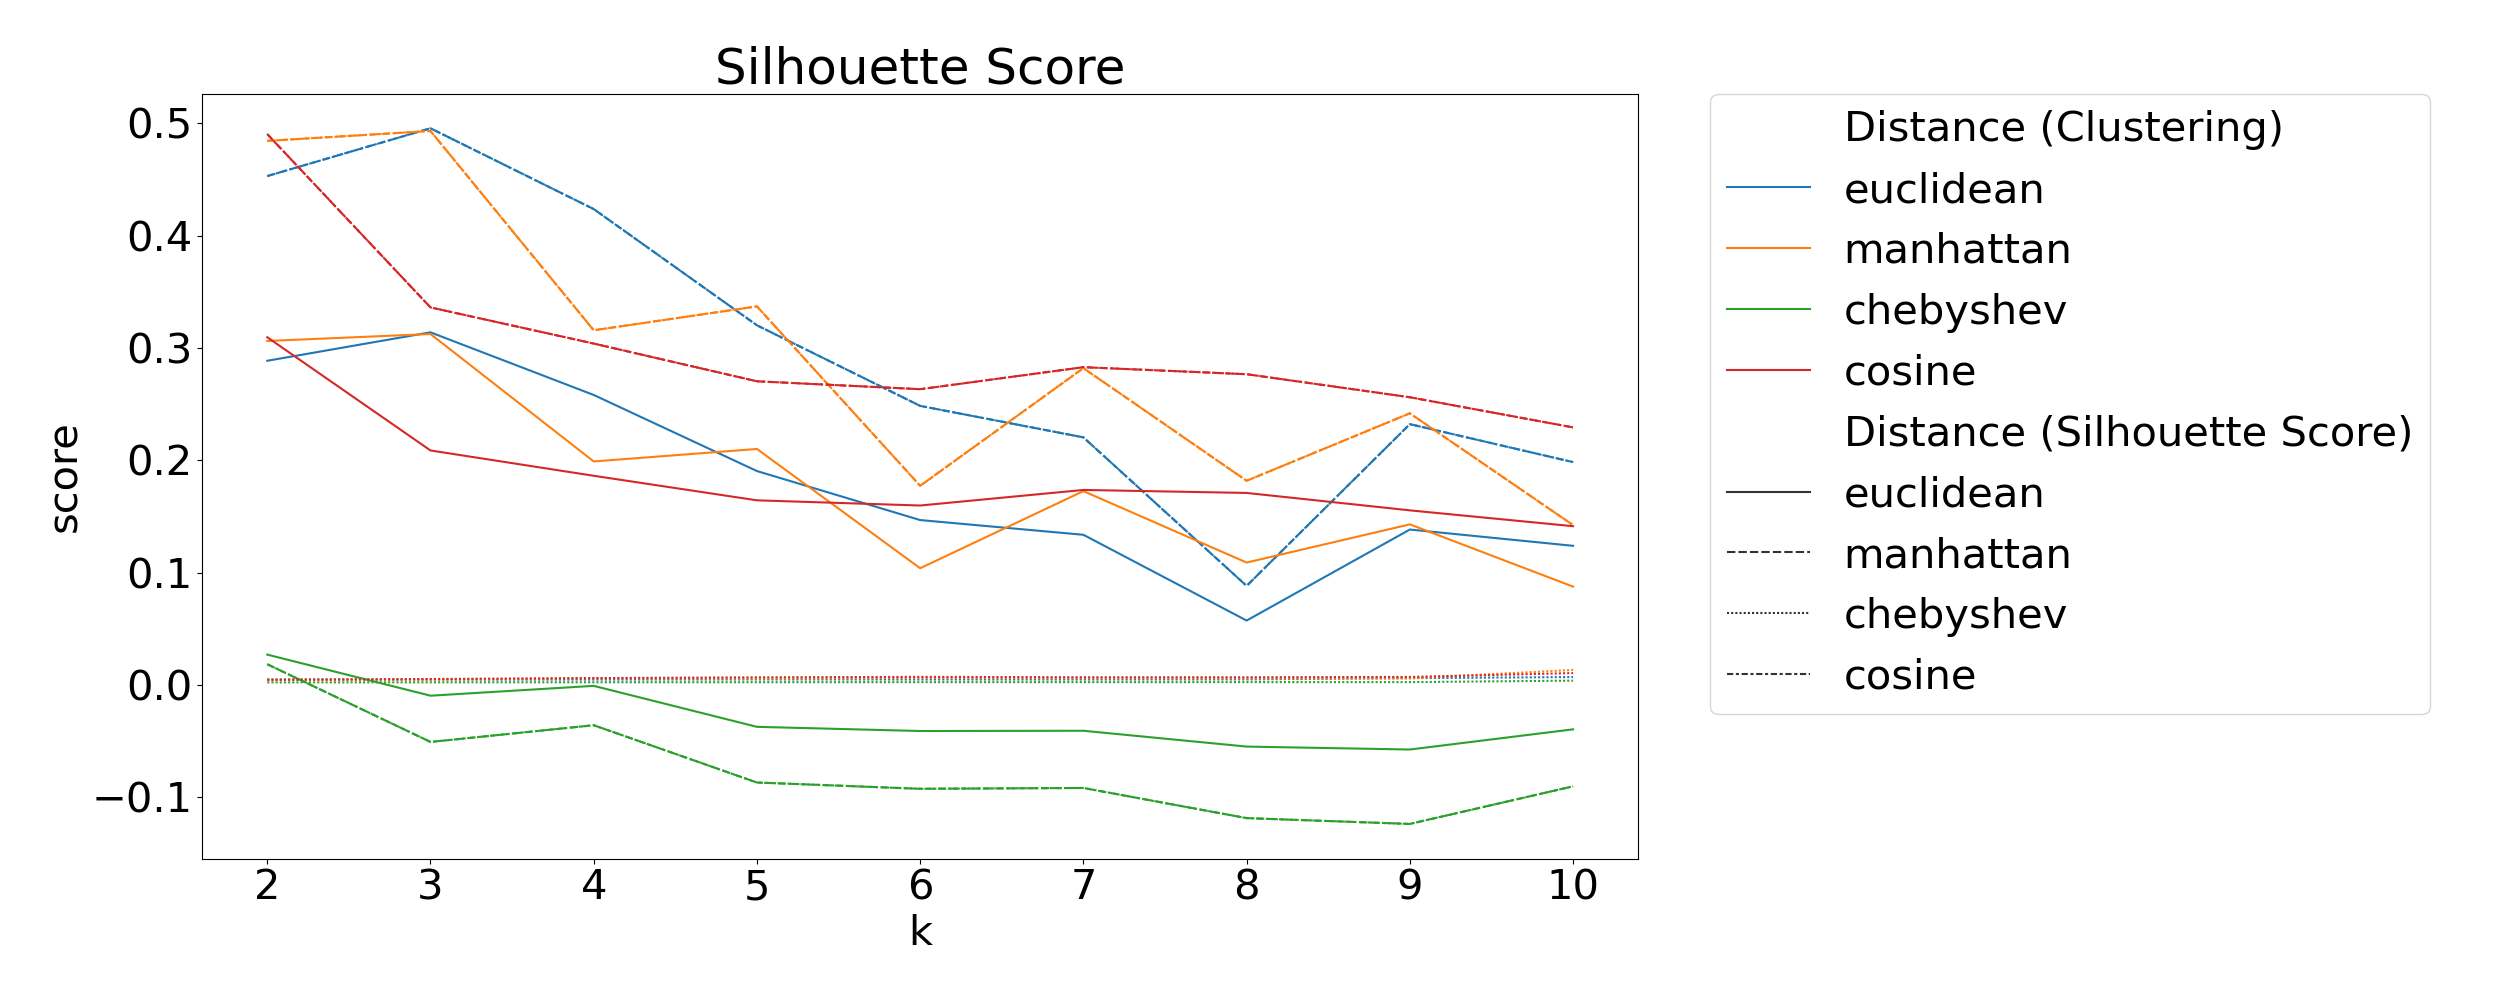
\includegraphics[width=1\textwidth]{../plots/housevotes/kmedians/Silhouette Score/k_1to10.png} }}%
	
	\caption{Comparison of clustering scores for kmedians-clustering on Housevotes dataset}%
\end{figure}

\begin{figure}[H]
	\centering
	\subfloat[ARI ]{{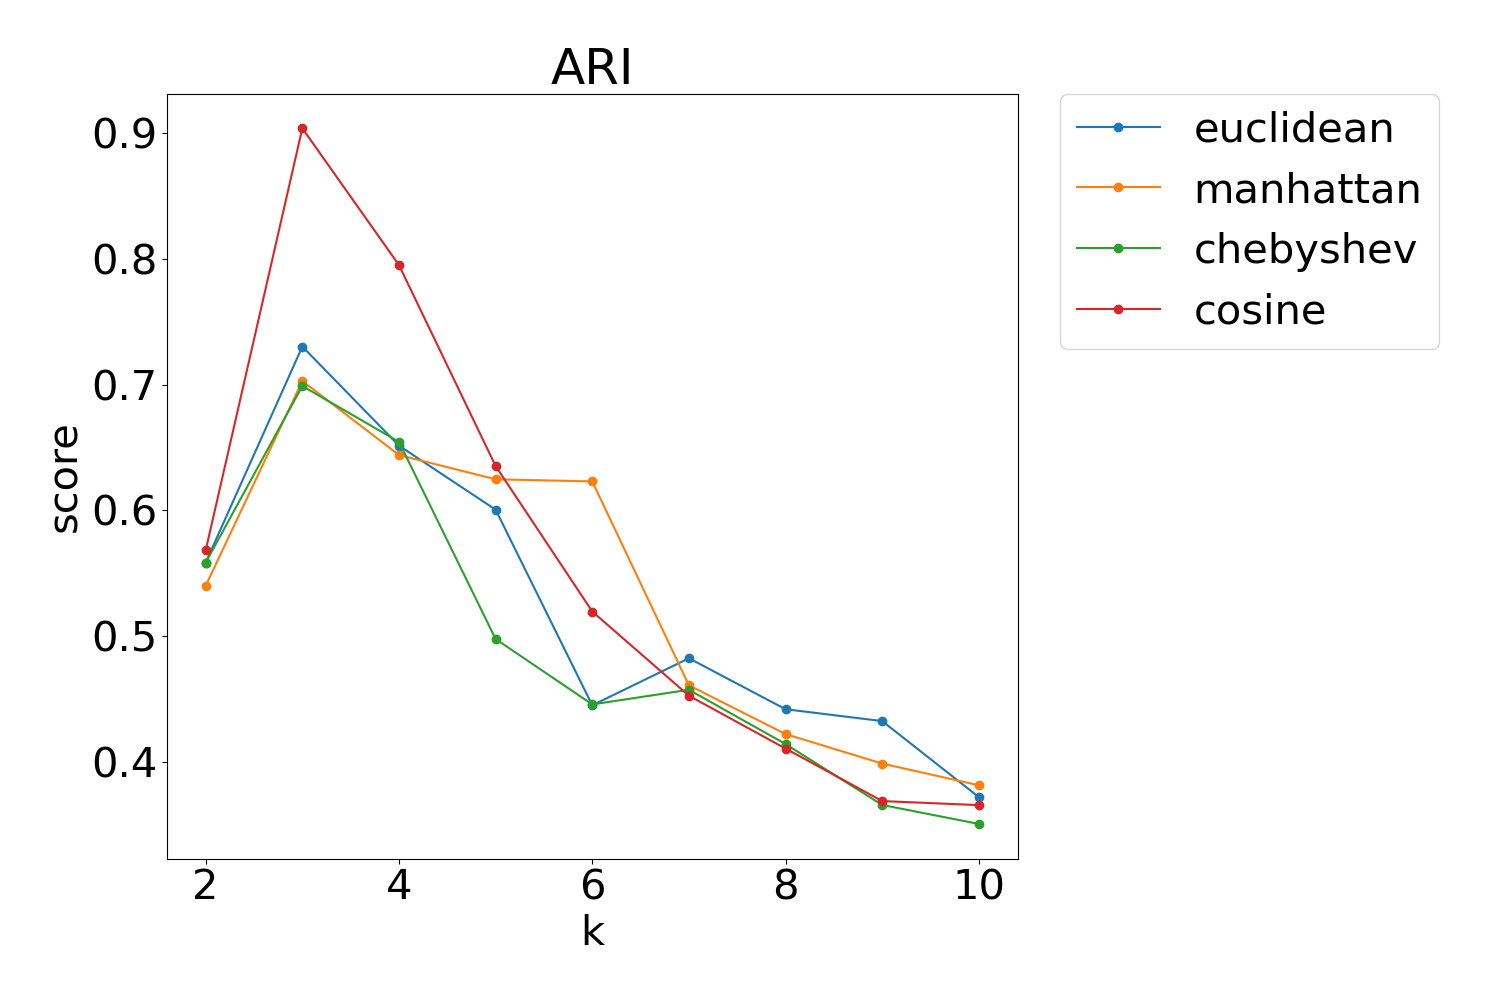
\includegraphics[width=0.45\textwidth]{../plots/iris/kmedoids/ARI/k_1to10.png} }}%
	\qquad
	\subfloat[NMI ]{{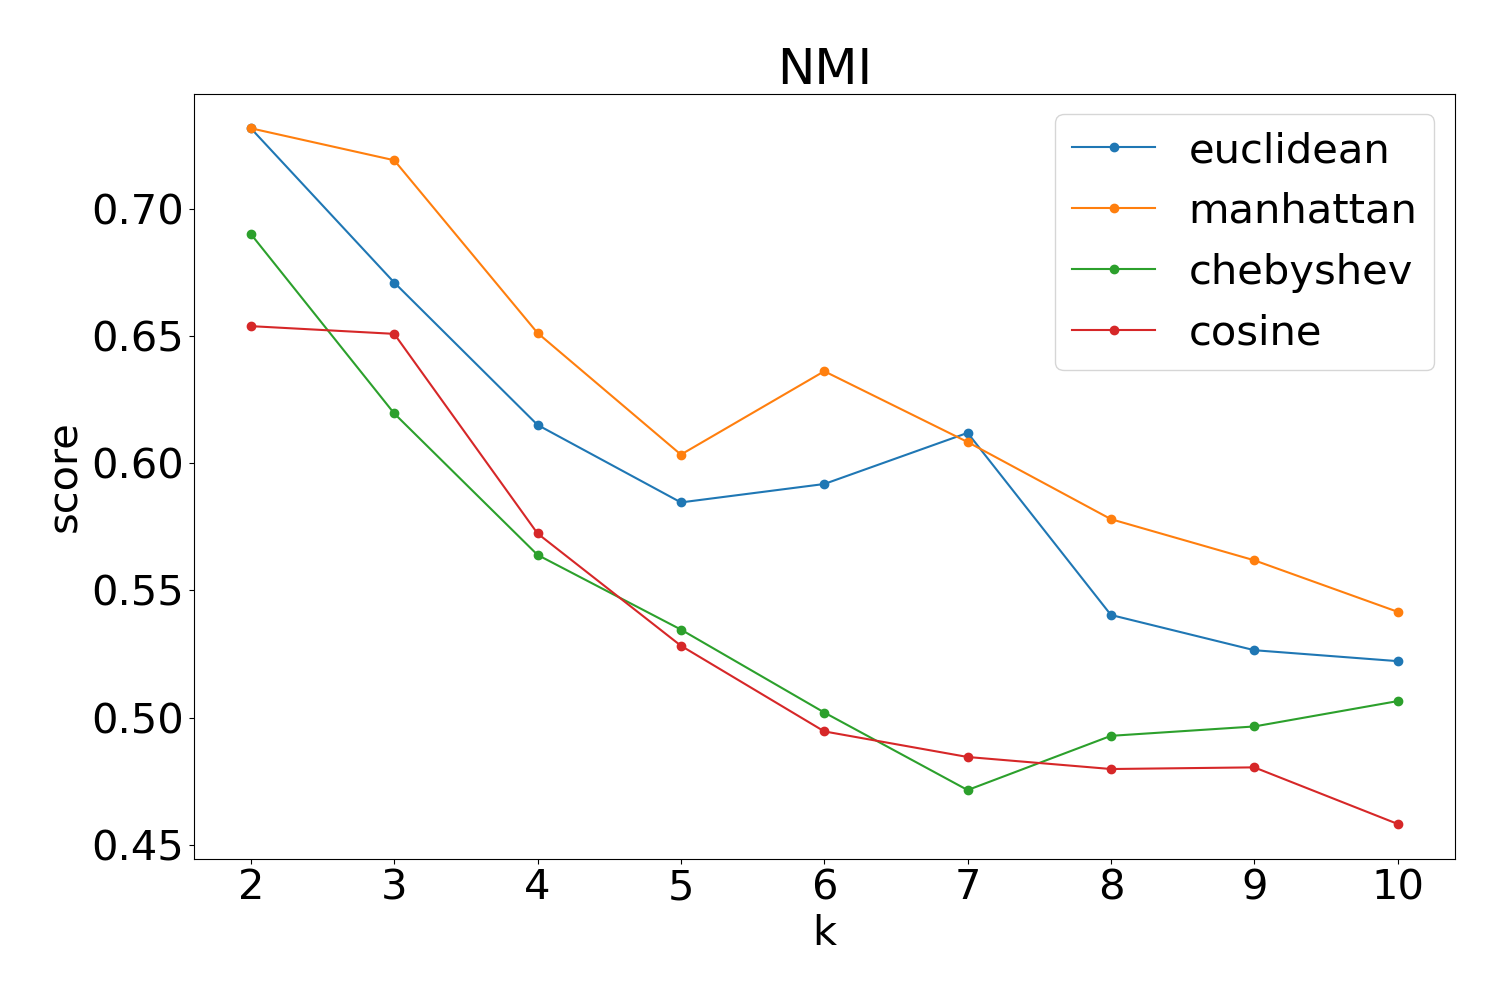
\includegraphics[width=0.45\textwidth]{../plots/iris/kmedoids/NMI/k_1to10.png} }}%
	\qquad
	\subfloat[Completeness Score ]{{\includegraphics[width=0.45\textwidth]{../plots/iris/kmedoids/Completeness Score/k_1to10.png} }}%
	\qquad
	\subfloat[Homogeneity Score ]{{\includegraphics[width=0.45\textwidth]{../plots/iris/kmedoids/Homogeneity Score/k_1to10.png} }}%
	\qquad
	\subfloat[Silhouette Score ]{{\includegraphics[width=1\textwidth]{../plots/iris/kmedoids/Silhouette Score/k_1to10.png} }}%
	
	\caption{Comparison of clustering scores for kmedoids-clustering on Iris dataset}%
\end{figure}

\begin{figure}[H]
	\centering
	\subfloat[ARI ]{{\includegraphics[width=0.45\textwidth]{../plots/wine/kmedoids/ARI/k_1to10.png} }}%
	\qquad
	\subfloat[NMI ]{{\includegraphics[width=0.45\textwidth]{../plots/wine/kmedoids/NMI/k_1to10.png} }}%
	\qquad
	\subfloat[Completeness Score ]{{\includegraphics[width=0.45\textwidth]{../plots/wine/kmedoids/Completeness Score/k_1to10.png} }}%
	\qquad
	\subfloat[Homogeneity Score ]{{\includegraphics[width=0.45\textwidth]{../plots/wine/kmedoids/Homogeneity Score/k_1to10.png} }}%
	\qquad
	\subfloat[Silhouette Score ]{{\includegraphics[width=1\textwidth]{../plots/wine/kmedoids/Silhouette Score/k_1to10.png} }}%
	
	\caption{Comparison of clustering scores for kmedoids-clustering on Wine dataset}%
\end{figure}

\begin{figure}[H]
	\centering
	\subfloat[Silhouette Score ]{{\includegraphics[width=1\textwidth]{../plots/diabetes/kmedoids/Silhouette Score/k_1to10.png} }}%
	
	\caption{Comparison of clustering scores for kmedoids-clustering on Diabetes dataset}%
\end{figure}

\begin{figure}[H]
	\centering
	\subfloat[ARI ]{{\includegraphics[width=0.45\textwidth]{../plots/housevotes/kmedoids/ARI/k_1to10.png} }}%
	\qquad
	\subfloat[NMI ]{{\includegraphics[width=0.45\textwidth]{../plots/housevotes/kmedoids/NMI/k_1to10.png} }}%
	\qquad
	\subfloat[Completeness Score ]{{\includegraphics[width=0.45\textwidth]{../plots/housevotes/kmedoids/Completeness Score/k_1to10.png} }}%
	\qquad
	\subfloat[Homogeneity Score ]{{\includegraphics[width=0.45\textwidth]{../plots/housevotes/kmedoids/Homogeneity Score/k_1to10.png} }}%
	\qquad
	\subfloat[Silhouette Score ]{{\includegraphics[width=1\textwidth]{../plots/housevotes/kmedoids/Silhouette Score/k_1to10.png} }}%
	
	\caption{Comparison of clustering scores for kmedoids-clustering on Housevotes dataset}%
\end{figure}




\subsection{Comparison for given k value}

For each dataset we independently compared clustering scores of different algorithms for multiple distances. For the algorithms that require a predefined number of clusters we set the value k to be the number of different classes in the dataset (except for the diabetes dataset, which does not have categorical labels). \\

\begin{figure}[H]
	\centering
	\subfloat[ARI ]{{\includegraphics[width=0.45\textwidth]{../plots/iris/combined/ARI/algdist_for_given_k.png} }}%
	\qquad
	\subfloat[NMI ]{{\includegraphics[width=0.45\textwidth]{../plots/iris/combined/NMI/algdist_for_given_k.png} }}%
	\qquad
	\subfloat[Completeness Score ]{{\includegraphics[width=0.45\textwidth]{../plots/iris/combined/Completeness Score/algdist_for_given_k.png} }}%
	\qquad
	\subfloat[Homogeneity Score ]{{\includegraphics[width=0.45\textwidth]{../plots/iris/combined/Homogeneity Score/algdist_for_given_k.png} }}%
	\qquad
	\subfloat[Silhouette Score ]{{\includegraphics[width=0.45\textwidth]{../plots/iris/combined/Silhouette Score/algdist_for_given_k.png} }}%
	
	\caption{Comparison of clustering scores for Iris dataset (given k=3)}%
\end{figure}

\begin{figure}[H]
	\centering
	\subfloat[ARI ]{{\includegraphics[width=0.45\textwidth]{../plots/wine/combined/ARI/algdist_for_given_k.png} }}%
	\qquad
	\subfloat[NMI ]{{\includegraphics[width=0.45\textwidth]{../plots/wine/combined/NMI/algdist_for_given_k.png} }}%
	\qquad
	\subfloat[Completeness Score ]{{\includegraphics[width=0.45\textwidth]{../plots/wine/combined/Completeness Score/algdist_for_given_k.png} }}%
	\qquad
	\subfloat[Homogeneity Score ]{{\includegraphics[width=0.45\textwidth]{../plots/wine/combined/Homogeneity Score/algdist_for_given_k.png} }}%
	\qquad
	\subfloat[Silhouette Score ]{{\includegraphics[width=0.45\textwidth]{../plots/wine/combined/Silhouette Score/algdist_for_given_k.png} }}%
	
	\caption{Comparison of clustering scores for Wine dataset (given k=3)}%
\end{figure}

\begin{figure}[H]
	\centering
	\subfloat[ARI ]{{\includegraphics[width=0.45\textwidth]{../plots/diabetes/combined/ARI/algdist_for_given_k.png} }}%
	\qquad
	\subfloat[NMI ]{{\includegraphics[width=0.45\textwidth]{../plots/diabetes/combined/NMI/algdist_for_given_k.png} }}%
	\qquad
	\subfloat[Completeness Score ]{{\includegraphics[width=0.45\textwidth]{../plots/diabetes/combined/Completeness Score/algdist_for_given_k.png} }}%
	\qquad
	\subfloat[Homogeneity Score ]{{\includegraphics[width=0.45\textwidth]{../plots/diabetes/combined/Homogeneity Score/algdist_for_given_k.png} }}%
	\qquad
	\subfloat[Silhouette Score ]{{\includegraphics[width=0.45\textwidth]{../plots/diabetes/combined/Silhouette Score/algdist_for_given_k.png} }}%
	
	\caption{Comparison of clustering scores for Diabetes dataset (given k=2)}%
\end{figure}

\begin{figure}[H]
	\centering
	\subfloat[ARI ]{{\includegraphics[width=0.45\textwidth]{../plots/housevotes/combined/ARI/algdist_for_given_k.png} }}%
	\qquad
	\subfloat[NMI ]{{\includegraphics[width=0.45\textwidth]{../plots/housevotes/combined/NMI/algdist_for_given_k.png} }}%
	\qquad
	\subfloat[Completeness Score ]{{\includegraphics[width=0.45\textwidth]{../plots/housevotes/combined/Completeness Score/algdist_for_given_k.png} }}%
	\qquad
	\subfloat[Homogeneity Score ]{{\includegraphics[width=0.45\textwidth]{../plots/housevotes/combined/Homogeneity Score/algdist_for_given_k.png} }}%
	\qquad
	\subfloat[Silhouette Score ]{{\includegraphics[width=0.45\textwidth]{../plots/housevotes/combined/Silhouette Score/algdist_for_given_k.png} }}%
	
	\caption{Comparison of clustering scores for Housevotes dataset (given k=2)}%
\end{figure}


\end{appendices}

\end{document}
